\documentclass{article}

\usepackage{textcomp}
\usepackage{tikz}
\usepackage{amsmath}
\usepackage{pdfpages}
\usepackage[hyphens]{url}
\usepackage{hyperref}
\usepackage[utf8]{inputenc}
\usepackage{relsize}
\usepackage{ifthen}
\usepackage{xstring}
\usepackage{cite}
\usepackage{placeins}
\usepackage{listings}
\usepackage{xcolor}
\usepackage{bold-extra}
\usepackage{amssymb}
\usepackage{booktabs}
\usepackage{rotating}
\usepackage{pdflscape}
\usepackage[inline]{enumitem}
\usepackage{mdframed}
\usepackage{mathtools}
\usepackage{bm}
\usepackage{newfloat}
\usepackage{xspace}

\newcommand{\crel}{
	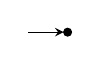
\begin{tikzpicture}[baseline={([yshift=-.8ex]current bounding box.center)}]
		\draw [->, >=stealth] (0,0) -- (0.45,0); 
		\draw [fill] (0.5,0) circle (0.05);
	\end{tikzpicture}
}

\newcommand{\rrel}{
	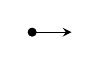
\begin{tikzpicture}[baseline={([yshift=-.8ex]current bounding box.center)}]
		\draw [fill] (0,0) circle (0.05);
		\draw [->, >=stealth] (0.05,0) -- (0.5,0);
	\end{tikzpicture}
}

\newcommand{\mrel}{
	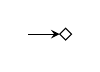
\begin{tikzpicture}[baseline={([yshift=-.8ex]current bounding box.center)}]
		\draw [->, >=stealth] (0,0) -- (0.4,0);
		\draw (0.4,0) -- (0.475,0.075) -- (0.55,0) -- (0.475,-0.075) -- cycle;
	\end{tikzpicture}
}

\newcommand{\irel}{
	\begin{tikzpicture}[baseline={([yshift=-.8ex]current bounding box.center)}]
		\draw [->, >=stealth] (0,0) -- (0.4,0);
		\draw (0.41,0) -- (0.55,0);
		\draw (0.48,-0.07) -- (0.48, 0.07); 
	\end{tikzpicture}
}

\newcommand{\erel}{
	\begin{tikzpicture}[baseline={([yshift=-.8ex]current bounding box.center)}]
		\draw [->, >=stealth] (0,0) -- (0.4,0);
		\draw (0.41,0) -- (0.55,0);
		\draw (0.48, 0.05) circle (0.02);
		\draw (0.48, -0.05) circle (0.02); 
	\end{tikzpicture}
}

\usepackage{amsmath}

\makeatletter
\DeclareFontFamily{U}{MnSymbolA}{}
\DeclareFontShape{U}{MnSymbolA}{m}{n}{
    <-6>  MnSymbolA5
   <6-7>  MnSymbolA6
   <7-8>  MnSymbolA7
   <8-9>  MnSymbolA8
   <9-10> MnSymbolA9
  <10-12> MnSymbolA10
  <12->   MnSymbolA12}{}
\DeclareFontShape{U}{MnSymbolA}{b}{n}{
    <-6>  MnSymbolA-Bold5
   <6-7>  MnSymbolA-Bold6
   <7-8>  MnSymbolA-Bold7
   <8-9>  MnSymbolA-Bold8
   <9-10> MnSymbolA-Bold9
  <10-12> MnSymbolA-Bold10
  <12->   MnSymbolA-Bold12}{}
\DeclareSymbolFont{MnSyA}{U}{MnSymbolA}{m}{n}
\SetSymbolFont{MnSyA}{bold}{U}{MnSymbolA}{b}{n}

\DeclareRobustCommand{\overleftharpoon}{\mathpalette{\overarrow@\leftharpoonfill@}}
\DeclareRobustCommand{\overrightharpoon}{\mathpalette{\overarrow@\rightharpoonfill@}}
\def\leftharpoonfill@{\arrowfill@\leftharpoondown\mn@relbar\mn@relbar}
\def\rightharpoonfill@{\arrowfill@\mn@relbar\mn@relbar\rightharpoonup}

\DeclareMathSymbol{\leftharpoondown}{\mathrel}{MnSyA}{'112}
\DeclareMathSymbol{\rightharpoonup}{\mathrel}{MnSyA}{'100}
\DeclareMathSymbol{\mn@relbar}{\mathrel}{MnSyA}{'320}
\makeatother

\newcommand{\MSG}[1]{\langle{#1}\rangle}
\newcommand{\REQ}[1]{\overrightharpoon{#1}}
\newcommand{\RSP}[1]{\overleftharpoon{#1}}
\newcommand{\ENUM}[1]{\texttt{#1}}
\newcommand{\COMMAND}{\ENUM{COMMAND}}
\newcommand{\APPEND}{\ENUM{APPEND}}
\newcommand{\POLL}{\ENUM{POLL}}
\newcommand{\ELECTION}{\ENUM{ELECTION}}


\newcommand\cpp{C\texttt{++}\xspace}

\DeclareFloatingEnvironment[
    fileext=los,
    listname=List of code snippets,
    name=Listing,
    placement=tbhp,
    within=none,
]{snippet}

\lstset{
  captionpos=b
 }

\definecolor{OliveGreen}{HTML}{3C8031}
\definecolor{Papyrus}{HTML}{FFFAE6}
\lstdefinestyle{pseudo}{
  mathescape=true,
  escapeinside={<|}{|>},
  morekeywords={function, send, to, receive, from, broadcast, timeout, match, with, when, and, or, if, else},
  morecomment=[l]{//},
  keepspaces=true,
  basicstyle=\small\ttfamily,
  commentstyle=\color{OliveGreen},
  keywordstyle=\color{blue}\bfseries,
  numberstyle=\small\ttfamily,
  numbers=left,
  xleftmargin=-.1cm
}

\begin{document}
\sloppy

\begin{titlepage}

	
\includepdf{itu-frontpage.pdf}

	\pagebreak

	\centering {\huge Trusted DCR: Decentralised workflow management in a byzantine setting}

	\vspace{1.5cm}

	{\large Mikkel Gaub \\ Malthe Ettrup Kirkbro \\ Mads Frederik Madsen}

	\vspace{0.5cm}

	\today

	\pagenumbering{gobble}

	\vspace{\fill}

	{\large Supervisor: Søren Debois}

	\vspace{0.5cm}

	\begin{abstract}
		In this thesis we present a solution to the problem of decentralized distributed workflow execution.
		The presented solution utilises partial state replication of dynamic condition response (DCR) graphs to achieve execution of events with complexity less than the number of peers in the system.
		We also explore the security and optimization options provided by recent advances in trusted execution environments (TEEs), specifically Intel Secure Guard Extensions (SGX), in order to achieve byzantine fault tolerance in the context of this problem.
		The design and implementation of this system contains several new contributions: a general transformation of crash fault tolerant distributed protocols to byzantine fault tolerant protocols using SGX, an SGX implementation of the Raft consensus algorithm, an efficient method of collecting the state of a DCR graph called \textit{CheapShot}, and an analysis of the synchronisation of executions in DCR graphs using a minimal locking scheme.
		Lastly we describe a generalisation of the implemented DCR graph system to a structure supporting arbitrary smart contracts.
	\end{abstract}
\end{titlepage}

\clearpage
\pagenumbering{arabic}

\tableofcontents

\newpage

\section{Introduction}

	Collaboration between companies, small and large, occurs daily across vast physical distances.
	As part of this collaboration a trusted means of coordination is key.
	One way to coordinate in such a setting is by using Dynamic Condition Response (DCR) graphs~\cite{hildebrandt_declarative_2011}, which are workflows declaratively formulated as directed graphs.
	DCR graphs formulate processes in terms of events and relations between those events.
	The relations specify the order in which events can transpire, and what paths can be taken in the workflow.

	DCR graphs provide a concise and simple way of describing workflows, as the effects of the execution of an event is explicitly defined by its relations.
	This means that an event execution cannot have cascading effects.
	This property of limited effects on execution means that DCR graphs allow for highly localized states and, depending on how a specific DCR graph is constructed, it can therefore allow for a very high degree of concurrency in a distributed setting.
	Central servers would be an easy way to enable a distribution of a workflow execution, but would introduce a single point of failure as well as require trust and most likely payment, due to a third party being involved in managing the process.

	The alternative to a solution using a central server is a decentralized solution, in which participants act as peers in a peer-to-peer network.
	Decentralisation brings with it a completely different set of challenges, all springing from the core necessity of distributed collaboration requiring agreement between all parties on what has transpired in the workflow.
	This set of challenges is the problem we will present and solve during this thesis.

	The issue of making DCR graphs distributed and maintaining a consistent state across peers is closely related to that of distributed replications of state machines, especially when peers can exhibit faulty behaviour.
	However, the ability for DCR graphs to allow a high degree of concurrency would be impeded by existing solutions to the distributed state machine replication (SMR) problem, due to the large number of messages required and the low degree of concurrency provided by the strict synchronisation of these algorithms.
	To improve on this strict synchronisation, different parts of the state can be distributed to different peers, thus allowing for synchronisation only between the parts of the state which affect each other.
	This is refereed to as the \textit{partial state machine replication} (PSMR) problem.

	Solutions to the PSMR problem are widely sought, as there are a number of applications of SMR solutions where the scalability of state is problematic.
	An example of this is the blockchain based distributed smart contract engine, Ethereum~\cite{_ethereum_2018}.
	We will therefore analyse the effects of applying our solution to the PSMR problem to an algorithm for running distributed smart contracts.

	Recent technological advances in the field of \textit{Trusted Execution Environments} (TEEs), specifically \textit{Intel Software Guard Extensions} (SGX)~\cite{costan_intel_2016}, have already made waves within state replication solutions~\cite{kapitza_cheapbft_2012,veronese_efficient_2013,liu_scalable_2016} and could potentially be leveraged to provide a solution to the described problem, efficiency in terms of required messages and a high degree of concurrency.
	Intel SGX provides a TEE in which arbitrary code can be run and the correct execution can be attested by Intel to other users also running Intel SGX.
	In a network of untrusting peers, trust can therefore be guaranteed by Intel, which is a very strong base to build a consensus algorithm on.

	\noindent The contributions of this thesis are as follows:
	\begin{itemize}
		\item An implementation of the Raft consensus algorithm inside of a TEE.
		\item A thorough design of a DCR engine, with a potentially totally distributed graph state\footnote{By event.}, supporting concurrent executions only limited by the semantics of DCR.
		Furthermore, the design accomplishes consensus on executions in less than $O(n)$ messages, where $n$ is the number of peers in the network.
		\item A proof-of-concept implementation of the former two.
		\item A transformation of any crash-stop tolerant distributed protocol to a byzantine fault tolerant one, using Intel SGX.
		\item A description of a generalised version of the DCR engine design supporting smart contracts.
	\end{itemize}

	\subsection{Problem}

	We formulate the problem of byzantine fault tolerant PSMR with a DCR graph as the \textit{state}, and allow for peers to collect the state and change the state through the execution of DCR events.
	In order to achieve fault tolerance, the system must distribute the DCR graphs on several peers, so that if one peer fails, other peers can take over correct execution of the DCR graph.
	The trivial method of ensuring fault tolerance, is to make all peers responsible for the entire state of the system, but means that changes in the graph would then have to be synchronized with all peers.
	For a solution to this problem to be scalable in large networks, a message complexity below $O(n)$ is desirable, where $n$ is the number of peers.
	Alternatively, the DCR graph would have to be split into parts distributed among peers, but this introduces further issues, as a partial state solution would need intermittent synchronization, when several actions might affect the same parts of the state.
	As DCR graphs are primarily used in industry where the documentation of workflows is important, it is essential that any user is able to collect the entire state of a workflow at any given time.
	Assuming a partial state solution, collecting this state is further complicated in that a coherent state would have to be pieced together from each part of the graph.

	In summary, the system should:
	\begin{description}
		\item[Concurrent] Allow for a high degree of concurrency as permitted by DCR graphs, shown in~\cite{debois_concurrency_2015}.
		\item[Scalable] Achieve consensus on a state change in less than $O(n)$ messages, where $n$ is the number of peers participating in the graph, while supporting the distribution of the state of the DCR graph among those peers.
		\item[Byzantine fault tolerant] Function in the presence of malicious workflow participants and network nodes, where the only guarantees are those based on strong cryptographic security.
	\end{description}

\section{Background}

In order to attain a complete understanding of the problem at hand, three subject areas need further explanation:
\begin{description}
	\item[DCR] which must be defined and the requirements of which must be explored, as it forms the basic limitations of a potential solution.
	\item[Consensus] which defines the fundamental challenge of any decentralized system, in which agreement on state is needed.
	\item[Intel SGX] which has recently shown promise in improving the fault tolerance of consensus solutions, notably in~\cite{kapitza_cheapbft_2012,veronese_efficient_2013,liu_scalable_2016}.
\end{description}

	\subsection{DCR}
	\label{subsec:dcr}

	A DCR graph $G$, is a graph representation of a workflow, made up of $v$ stateful nodes, $E=\{e_1, e_2, \dots, e_v\}, v \geq 1$, called \textit{events}, with a number of directed edges called \textit{relations} between them.
	The cumulated state of all the events in a graph $G$ is called the state of $G$.
	Depending on the relations, an event $e$, in a graph $G$, can be \textit{executed}, which will change the state of events in $G$ according to the rules defined by $e$'s outgoing relations.
	We denote this execution $E(G,e)=G'$.

			\subsubsection{Event State}

			The events in a DCR graph have three binary attributes: \textit{executed}, \textit{included} and \textit{pending}.
			This is an event: \ev{A}

			\begin{description}
				\item[Executed attribute] If the \textit{executed} attribute of an event is false, executing the event will set its \textit{executed} attribute to true.
				Executing an already executed event will have no effect on the \textit{executed} attribute.
				The \textit{executed} attribute is shown as a tick mark: \ev[101]{A}
				\item[Included attribute] If the \textit{included} attribute is true, the event is said to be \textit{included}.
				If the \textit{included} attribute of an event is false, the event is said to be \textit{excluded} and it cannot be executed.
				The \textit{included} attribute is denoted by the outline of the event: \ev{A} when included and \ev[000]{A} when excluded.
				\item[Pending attribute] If any event in a workflow has a \textit{pending} attribute which is true and that event is included, we expected further executions of events in the workflow and say that the workflow is in an unfinished state.
				Every time an event is executed, its \textit{pending} attribute is set to false.
				This means that setting the \textit{pending} attribute of an included event to true is specifying that this event must be executed or excluded at some point to leave the workflow in a finished state.
				The \textit{pending} attribute is shown as an exclamation point: \ev[011]{A}
			\end{description}

			\subsubsection{Relations}
			\label{subsubsec:relations}

			Relations are directed edges between events in the workflow.
			Each relation is directed from an origin event, toward a target event.
			There are five types of relations which each specify different behaviour between events in a workflow.
			The origin and the target of a relation can be the same event.
			The relations can be divided into two categories:

			\begin{description}
				\item[Effects] are relations that change the state of the targeted event when the originating event is executed.
				If an effect originating from an event \texttt{A} is targeting an event \texttt{B}, then \texttt{A} is said to be the effecting event on the effected event \texttt{B}.
				Effects are the \emph{response}, \emph{include} and \emph{exclude} relations.
				\begin{description}
					\item[Response relation] If there is a response relation from event \texttt{A} to event \texttt{B}, then the \textit{pending} attribute of \texttt{B} will be set to true every time \texttt{A} is executed.
				The response relation is represented as: $\ev{A} \rrel \ev{B}$
					\item[Include relation] If there is an include relation from event \texttt{A} to event \texttt{B}, then the \textit{included} attribute of \texttt{B} will be set to true every time \texttt{A} is executed.
				The include relation is represented as: $\ev{A} \irel \ev{B}$
					\item[Exclude relation] If there is an exclude relation from event \texttt{A} to event \texttt{B}, then the \textit{included} attribute of \texttt{B} will be set to false every time \texttt{A} is executed.
				The exclude relation is represented as: $\ev{A} \erel \ev{B}$
				\end{description}
				\item[Constraints] are relations that exclusively affect whether or not the targeted event can be executed.
				If a constraint originating from an event \texttt{A}, is targeting an event \texttt{B}, then \texttt{A} is said to be the constraining event on the constrained event \texttt{B}.
				Constraints are the \emph{condition} and \emph{milestone} relations.
				\begin{description}
					\item[Condition relation] If there is a condition relation from event \texttt{A} to event \texttt{B}, then \texttt{B} can only be executed if the \textit{executed} attribute of \texttt{A} is true or the \textit{included} attribute of \texttt{A} is false.
				The condition relation is represented as: $\ev{A} \crel \ev{B}$
					\item[Milestone relation] If there is a milestone relation from event \texttt{A} to event \texttt{B}, then \texttt{B} can only be executed if the \textit{pending} attribute of \texttt{A} is false or the \textit{included} attribute of \texttt{A} is false.
				The milestone relation is represented as: $\ev{A} \mrel \ev{B}$
				\end{description}
			\end{description}

			\subsubsection{Enabledness}

			We use the notion of \textit{enabledness} to describe whether an event is executable in the state of a given graph or not.
			An event is \textit{enabled} if it can be executed, and \textit{disabled} if it cannot.
			An event's enabledness is strictly controlled by the state of its constraining events, and its included variable:
			\begin{itemize}
				\item If an event is excluded it is disabled.
				\item If an event is the target of a milestone relation from an event that is included and pending, it is disabled.
				\item If an event is the target of a conditions relation from an event that is included and not executed, it is disabled.
			\end{itemize}
			In all other cases, the event is enabled.

			\subsubsection{Formalising \texorpdfstring{$G$}{}}
			\label{subsubsec:formalising-g}

			After the previous definitions, we can now formalise the concept of a DCR graph $G$:
			$G = (E,R)$, where
			\begin{itemize}
				\item $E$ is the set of all events in the workflow,
				\item $R = \{r_1, r_2, \dots\}$ is the set of relations in the workflow, where each relation, $r$, has the form $r=(e_{from}, e_{to}, Type)$ and $e_{from}$ is the event $r$ is originating from, $e_{to}$ is the event $r$ is targeting, and $Type$ is one of the relation types described in Section~\ref{subsubsec:relations}.
			\end{itemize}

			If, in a given state of $G$, an event $e'$ changes state or enabledness when event $e$ is executed, we say that $e'$ is in $e$'s \textit{effecting event set}, denoted $E_{eff}(G,e)$.

			\subsubsection{Concurrency}
			\label{subsubsec:concurrency}

			The notion of concurrency in DCR graphs, described in~\cite{debois_concurrency_2015}, is the property a pair of events have when the graph allows those events to be executed in either order with the same resulting graph state.

			More formally, given a graph $G$ and two events $e_1$ and $e_2$ in $G$, we say that $e_1$ and $e_2$ are concurrent if $E(E(G, e_1),e_2)=E(E(G, e_2),e_1)$.

			We define a \textit{run} as a series of consecutive executions.
			For a run to be valid, each execution must be enabled at the point of execution in the sequence.
			We say that two runs $R_1$ and $R_2$, containing the same set of executions, are \textit{equivalent up to concurrency} on a graph $G$ when the results of performing $R_1$ on $G$ leads to $G'$ and performing $R_2$ on $G$ also leads to $G'$.
			If there exist a run $R$ which applied to a graph state $G$ results in graph state $G'$, we say that $G'$ is \textit{reachable} from $G$ via $R$.

			We identify three concurrency relationships between events, and name these relationships \textit{independence relationships}, and say that the events in an independence relationship are \textit{independent}:
			\begin{description}
				\item[Dynamic independence] Two events are \textit{dynamically independent} if they are both enabled and concurrent in the current state of the graph.
				That is, $e_1$ and $e_2$ are dynamically independent if $E(E(G, e_1),e_2)=E(E(G, e_2),e_1)$ for the current $G$.
				Dynamic independence is essentially what we have defined as concurrency.

				We say that an event $e$ has a \textit{dynamic independence set} $I_{dyn}(G,e)$, such that $e' \in I_{dyn}(G,e)$ iff. $e$ and $e'$ are dynamically independent in graph state $G$.
				Likewise an event $e$ has a \textit{dynamic dependence set} $D_{dyn}(G,e) = E \setminus I_{dyn}(G,e)$.

				\item[Static independence] Two events are \textit{statically independent} if they are dynamically independent in every \textit{reachable} state of the graph from the initial graph state.
				That is, $e_1$ and $e_2$ are statically independent in $G$, if they are dynamically independent in all states of $G$ that can be reached by a run.

				We say that an event $e$ has a \textit{static independence set} $I_{stat}(e)$, such that $e' \in I_{stat}(e)$ iff. $e$ and $e'$ are statically independent.
				Likewise an event $e$ has a \textit{static dependence set} $D_{stat}(e) = E \setminus I_{stat}(e)$.
				Notice that $e$'s static dependence set is the set of events that are dependent with $e$ in \textit{some} state of $G$, not all.
				The problem of finding all static independence sets is NP-hard in~\cite{debois_replication_2017-1} and an approximation will have to be used instead.
			\end{description}

			The approximation we use of static event independence is from~\cite{debois_concurrency_2015}, and boils down to the following principles, where we say that $e_1$ and $e_2$ are approximately statically dependent if, in any event-state permutation of $G$:
			\begin{itemize}
				\item $e_1$ can enable $e_2$, or vice versa.
				\item $e_1$ can disable $e_2$, or vice versa.
				\item $e_1$ can disable some $e$, if $e_2$ can enable it, or vice versa.
				\item $e_1$ can exclude some $e$, if $e_2$ can include it, or vice versa.
				\item $e_1$ can set $e_2$ to pending, unless $e_2$ sets itself to pending, or vice versa.
			\end{itemize}
			This approximation is complete, but not sound, meaning it contains all statically dependent event pairs, but does not guarantee that an event pair in the approximation is not statically independent.
			We say that an event $e$ has an \textit{approximate static dependence set} $D_{appr}(e)$, such that $e' \in D_{appr}(e)$ iff. $e$ and $e'$ are approximately statically dependent, according to the above approximation.
			Likewise an event $e$ has an \textit{approximate static independence set} $I_{appr}(e)  = E \setminus D_{appr}(e)$.
			Notice that the an approximate static independence set is sound but incomplete.

			All the independence- and dependence sets are symmetric: $e' \in S(e) \iff e \in S(e')$, where $S$ is any of the described (in-)dependency sets.
			Notice that in any DCR graph it must hold that $\forall G. \forall e\in G. |I_{dyn}(G,e)| \geq |I_{stat}(e)| \geq |I_{appr}(e)|$, which speaks to the desirability of the different concurrency levels; a system that supports concurrent execution of dynamically independent events allows for more concurrent executions than a one that supports execution of statically independent events, which in turn allows for more concurrent executions than one that supports execution of approximate statically independent events.
			Figure~\ref{fig:concurrency-all} shows examples of independence in DCR graphs.

		\begin{figure}[!ht]
			\center
			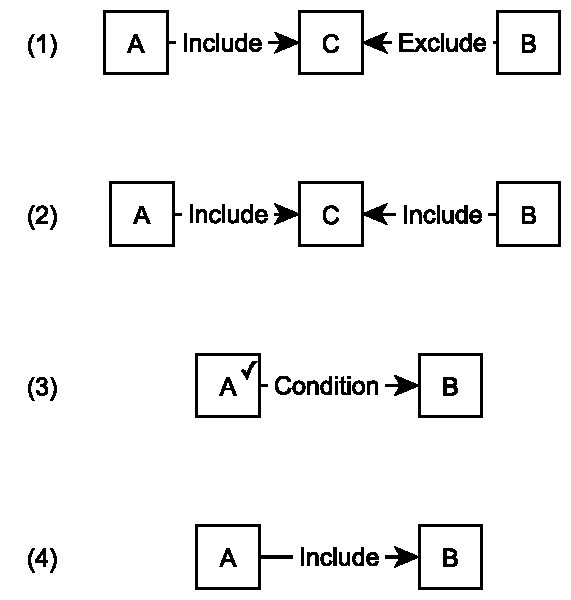
\includegraphics[scale=0.6]{figures/dcr-graphs/concurrency-all.pdf}
			\caption{From top to bottom:
			(1) An example of a DCR graph where \ev{A} and \ev{B} are not concurrent.
			(2) An example of a DCR graph where \ev{A} and \ev{B} are statically independent.
			(3) An example of a DCR graph where \ev{A} and \ev{B} are dynamically, but not statically independent.
			(4) An example of a DCR graph where \ev{A} and \ev{B} are statically independent, but the approximation will contain them as a dependent pair\label{fig:concurrency-all}.}
		\end{figure}

			\subsubsection{Execution rights}

			For DCR graphs to have a meaningful application, each event is typically assigned a number of actors who are allowed to execute that event.
			Rights to execute can also be assigned based on role.

		\subsection{Consensus}
		\label{subsec:consensus}

		Consensus is the problem of achieving agreement between the processes in a distributed system.
		It is central to the problem of decentralised DCR, as agreement on the states of events must be achieved to ensure that all correct peers adhere to the semantics of the DCR graph.

		Consider a simple graph: $\ev{A} \crel \ev{B}$, and let a subset of peers, $ps_1$, store the state of $\ev{A}$, and a subset of peers, $ps_2$, store the state of $\ev{B}$.
		If agreement on the state of $\ev{A}$ is not guaranteed, then $ps_2$ might, in the belief that $\ev{A}$ is executed, execute $\ev{B}$ even though $ps_1$ has never executed $\ev{A}$.

		A consensus protocol is formally a protocol with $n$ processes ($p_1, p_2, \dots, p_{n}$), where each process $p_i$ begins in an undecided state, and proposes a single value $v_i$ from a set of values $D$. The processes then communicate their values to each other, and each process sets a decision value $d_i$ and enters a decided state.
		For the protocol to solve the consensus problem, the following requirements should hold for every execution:
		\begin{description}
			\item[Termination] every process eventually sets its decision value.
			\item[Agreement] the decision value of all correct processes are the same.
			\item[Validity] if a correct process decides $d$, then some correct process has proposed a value $v$, where $v = d$.
		\end{description}

		We show that distributed DCR reduces to consensus, under the assumptions that the correct graph has been distributed to all peers, and that the initial state is agreed upon:
		\begin{itemize}
			\item Let $D$ be the set of enabled events.
			\item Let $v_i$ uniquely identify an event.
			\item A correct process will only propose $v_i$ if the event identified by $v_i$ is enabled.
			\item We can now use a consensus sub-process to decide on a $v$, which will then be executed.
			\item Each process recalculates $D$ to reflect the new global state, and repeats the protocol until the workflow has been completed.
		\end{itemize}

		In the famous FLP impossibility result from 1985~\cite{fischer_impossibility_1985}, it was shown that no consensus protocol could have termination, agreement and validity.
		The proof essentially boils down to showing that that non-termination is possible in all consensus protocol systems with asynchronous communication channels and at least one faulty process.
		In order to circumvent this impossibility, the guarantees of a fault-tolerant system that utilizes a consensus protocol must be relaxed, for instance by guaranteeing termination only when no faults are present, as is the case in the Paxos protocol~\cite{lamport_part-time_1998}.

		\subsubsection{State Machine Replication}

		One problem that relates directly to consensus, is \textit{State Machine Replication}~\cite{schneider_implementing_1990} (SMR).
		SMR is the problem of replicating the state of a system on several nodes, called \textit{replicas}.
		On each replica, an instance of the same state machine is running, and must take requests and pass them on to the state machine.
		In SMR systems, \textit{clients} send requests to the replicas who must then guarantee:
		\begin{description}
			\item[Safety] all non-faulty replicas execute the requests in the same order.
			\item[Liveness] clients eventually receive replies to their requests.
		\end{description}
		The state machine replication problem is equivalent to the consensus problem and provides the same guarantees~\cite{schneider_implementing_1990}, since a solution to SMR is consensus on the state of a request log.
		This is evident in the fact that the safety requirement is essentially an aggregation of the agreement and validity requirements in consensus, while the liveness property is equivalent to termination.
		As such, FLP impossibility entails that one of the requirements must be relaxed in fault tolerant SMR systems.
		This is often done by only guaranteeing liveness when no failures are present~\cite{chandra_unreliable_1996,lamport_part-time_1998,castro_practical_1999,kotla_zyzzyva_2007}.

		A version of SMR deals with byzantine faults, rather than crash failures.
		These systems are knowns as \textit{byzantine fault tolerant} (BFT) systems~\cite{castro_practical_1999,correia_byzantine_2011,veronese_efficient_2013,liu_scalable_2016}.
		These systems deal with arbitrary faults, meaning arbitrary behaviour of faulty processes and channels, including modified messages, new messages and changes in local state.
		It has been shown that $2f+1$\footnote{Reads as $n=2f+1$, where $n$ is the number of processes, and $f$ is the number of recoverable faults.} processes are necessary and sufficient to solve SMR with relaxed liveness if faulty processes only exhibit crashes~\cite{bracha_asynchronous_1985}.
		Similarly it has been shown that $3f+1$ processes are necessary and sufficient to solve SMR with relaxed liveness if faulty processes can exhibit byzantine faults~\cite{bracha_asynchronous_1985,pease_reaching_1980}.
		However, recent advances have been made in BFT-algorithms, which increase fault tolerance from $3f+1$ to $2f+1$ by utilizing TEE features~\cite{liu_scalable_2016,kapitza_cheapbft_2012,veronese_efficient_2013}.

		SMR brings with it the taxing job of pushing each update to all nodes in the network, which leads to obvious scalability issues in large networks.
		One solution to that problem is delegating the responsibility of segments of data to each node in the network.
		This is called \textit{Partial State Machine Replication} (PSMR)~\cite{sousa_partial_2001}.
		Since the state in PSMR is divided into parts, it is possible for multiple leaders to be active concurrently, as opposed to traditional SMR implementations, that have a single leader at any given time.
		Having multiple leaders means that the availability of the system is much greater, as a single node does not have to process all requests.
		High concurrency and performance also follows from the partial states reducing the number of nodes which have to be notified of a state change leading to both fewer messages and less chance of two state changes overlapping, requiring ordering.
		Relatively few solutions exists for the PSMR problem and the ones that do require a large amount of messages~\cite{sousa_partial_2001}.
		To the best of our knowledge, no solution to the PSMR problem using a trusted execution environment exists.

		\subsection{Intel Software Guard Extensions}
		\label{subsec:intel-sgx}

		Intel SGX is a TEE technology which includes a set of CPU instructions, that allow user-level code to run in protected areas of memory, so called \textit{enclaves}.
		Only processes running in enclaves are allowed to use SGX instructions.
		Intel guarantees that any code run within an enclave, and any data loaded into an enclave, is protected from access by any process running outside of that enclave~\cite{intel_sgx}.
		More specifically, the guarantees encompass \textit{confidentiality}, as only the process running in the enclave can read the contents of the enclave, and \textit{integrity}, as only the process running in the enclave can modify the contents of the enclave.
		These guarantees of the enclave comes at the expense of direct access to system calls, and by extension drives, network cards and all hardware components other than the processor it runs on.
		In order to access any of these, an enclave therefore needs a so-called \textit{wrapper component} which is a non-enclave block of memory that the process can make calls to, and receive calls from.

		This is all made possible by a set of unique keys generated during manufacturing and permanently stored inside the so-called \textit{fuse array} of the processor | an array of fuses that can be programmed once and then protected from further manipulation~\cite{robson_electrically_2007}.
		Using these keys, an enclave process is able to identify if another process is an enclave process, using the process of \textit{local attestation}.
		Local attestation is intuitively possible as two enclaves running on the same processor both have access to the same secret key, provisioned by Intel.
		This process can be extended to identify if a process running on another processor is an enclave process, by contacting Intel's servers for verification of the other processor's key, called \textit{remote attestation}.
		Remote attestation can be performed with all other SGX enabled processes, as Intel has already provisioned keys to these.

		In short, the major innovation in Intel SGX is the option of running hardware secured software, which enables tamper-proof messages, where the sender can be verified as being a correct process.

		As an example of SGX's usefulness in relation to consensus algorithms, SGX has been utilized to implement a new Byzantine fault tolerance (BFT) consensus algorithm, called \textit{FastBFT}~\cite{liu_scalable_2016}.
		This is accomplished by using the \textit{strawman design} where a request is sent to a node, the \textit{primary}, who prepares a vote by distributing parts of a secret to all nodes.
		The secret can be reconstructed given enough parts and then compared to the hash of the secret which is common knowledge.
		The reason that Intel SGX is needed for this algorithm is that the primary, who distributes the secrets, can fake being any node as it has all parts of the secret.
		A Trusted Execution Environment (TEE) such as Intel SGX, means that these secrets can be computed and distributed without the primary ever having access to them.
		A further issue with the strawman design, is that the primary can change the orders of requests, thereby equivocating which request is being voted on.
		This is once again solved by Intel SGX, by numbering requests with a trusted counter that can only be incremented.
		This application of Intel SGX means that the byzantine faults in the algorithm, $f$, can now be tolerated up to $f = \lfloor\frac{n-1}{2}\rfloor$, given that the SGX component does not exhibit byzantine faults, but at most crash faults.

			\subsubsection{Enclave}
			\label{subsec:enclave}

			An enclave is a software module which, as its name suggests, is isolated completely from the rest of the system.
			The strong guarantees of enclaves, confidentiality and integrity, build on the following two hardware details:
			\begin{description}
				\item [Processor Reserved Memory (PRM)] is a sequential block of memory reserved for SGX, only accessible through enclave CPU instructions.
				\item [Enclave mode] is a mode under which a process gains access to the PRM.
			\end{description}
			An enclave's memory is located solely in PRM, preventing access by other processes and enclaves running on the system.
			The PRM is protected from non-enclave processes by enclave mode.
			When a process is not in enclave mode and tries to access the PRM, the memory access is denied by the processor~\cite{costan_intel_2016}.
			The PRM of an enclave process is protected from accesses by other processes in enclave mode by the SGX Enclave Control Structure (SECS).
			The SECS holds meta-data about the enclave processes, and among this is a virtual-to-physical memory mapping called the Enclave Page Cache (EPC).
			Through the EPC an enclave's access to physical PRM is restricted to what has been allocated for the enclave-process~\cite{costan_intel_2016}.
			All enclave data is encrypted while stored in memory, and is decrypted when loaded out of memory, and as such prevents anyone from reading the enclave data by bypassing the processor.

			While SGX provides powerful guarantees through its enclave concept, it does not guarantee software correctness and will not protect against flawed software.
			Instead SGX encourages developers to isolate a minimal piece of their software, the Trusted Computing Base (TCB), in a trusted enclave environment, and keep the remainder outside the enclave~\cite{intel_sgx_guide}.
			By minimizing the size of the TCB, and thus the amount of code one must trust, common security principles dictate that the chance of security flaws decreases~\cite{intel_sgx_guide}.

			In order for an enclave to be useful, communication with untrusted code is typically required.
			Calls to trusted enclave code from untrusted code, or other enclaves, is enabled through \textit{enclave calls} (ECALLs) and calls to untrusted code from enclave code is enabled through \textit{out calls} (OCALLs).
			This interface must be defined at compile-time, specifying an API of ECALLs for the enclave as well as any untrusted services needed as OCALLs, in an \textit{EDL}-file~\cite{intel_sgx_guide}.

			When built, an enclave module is a plain binary on the untrusted file system.
			As an enclave under such circumstances would be vulnerable to tampering before initialization, SGX enforces a strict signature policy.
			An enclave must include an \textit{Enclave Signature} containing \textbf{(1)} a hash of the code and initialization data of the enclave, \textbf{(2)} the author's public key and \textbf{(3)} an enclave version/product number.
			During enclave initialization a hardware check is performed, ensuring that the Enclave Signature matches the enclave binary loaded from the file system.
			This signature identifies the enclave during the attestation process as well, so if an adversary was to tamper with an existing enclave binary, the contents would no longer match, and would not be allowed to be loaded by SGX.
			If the adversary was to create their own enclave, replacing the existing, the signature would no longer match and the replacement would be rejected during the attestation process with other, correct, enclaves.

			Another powerful tool of an SGX enclave is the ability to read from, and write data to, an untrusted storage medium while ensuring confidentiality of its contents.
			Such capabilities are needed as the PRM is volatile and will not persist after shutdown.
			In SGX this process is known as \textit{sealing}.
			Sealing allows encryption and decryption using a \textit{Seal Key}, which is confidential to the sealing enclave.

			However, these mechanics alone do not guarantee integrity, as integrity is not only violated by other processes.
			For instance, the infamous Single Upset Event (also knowns as cosmic ray bit flips)~\cite{normand_single_1996}, is an integrity violation where bits in memory are flipped due to background radiation.
			Intel SGX protects against such hardware errors by using cryptographic integrity checks~\cite{gueron_memory_2016}.
			When loading enclave memory, Intel SGX's Memory Encryption Engine (MEE) decrypts the memory, and then performs an integrity check on the loaded memory.
			If the integrity check does not pass, the processor drops the memory, and eventually locks itself for further operations (the \textit{drop-and-lock policy}), requiring a physical reset before new operations can be completed~\cite{jang_sgx-bomb_2017}.

			The integrity checks are implemented as a Merkle-Tree of Message Authentication Codes (MACs), with the root node of the tree stored in processor-internal memory~\cite{jang_sgx-bomb_2017}.
			Under the assumption that AES128 is a random permutation, this method provides the guarantee that an active adversary with the capability of observing the MACs has a negligible probability of forgery~\cite{gueron_memory_2016}.

			A practical example of the effectiveness of this integrity check is the \textit{SGX bomb} attack~\cite{jang_sgx-bomb_2017}.
			The SGX bomb, is a denial-of-service attack on Intel SGX.
			It utilises a Row hammer attack to flip arbitrary bits in the EPC, thus triggering the drop-and-lock policy whenever memory is loaded.

			\subsubsection{Attestation}
			\label{subsec:attestation}

			Attestation, within the Intel SGX platform, is the action of verifying that some other process is running inside a specific enclave.
			The applications of this are two-fold, in the case where there are multiple enclaves running locally on the same CPU and in the case where enclaves need to communicate to enclaves running on external CPUs.
			These two situations are handled by two different processes, aptly named local and remote attestation.

			Local attestation builds on a secret fused into the CPU.
			An enclave can use an SGX instruction to generate a \textit{report} uniquely identifying the enclave, as it also contain the enclave signature.
			This report is MACed with a key derived from the fused secret and enclave identifier.
			It is not possible to use the create such a report for another enclave, as the report instruction is only available to software components that ensure that the report corresponds to the caller enclave.
			The fused secret is not directly accessible by software components, but can only be used by certain hardware instructions that protects against malicious use~\cite{costan_intel_2016}.
			An attestation challenger will ask for a MAC'ed report from the client enclave, and after receiving it derive the same key to verify the MAC.
			Because a report can only be created by the enclave it describes, the challenger can be certain of which enclave the client is running if the MAC is valid.
			To prevent replays the MAC'ed report is allowed to contain a block of arbitrary data, in which the challenger can require a nonce~\cite{costan_intel_2016}.

			Remote attestation builds on the same concept of a report, but as challenger and client are now on different CPUs, they no longer hold the same fused secret.
			Instead remote attestation relies on the group signature scheme Enhanced Privacy ID (EPID) and a third party issuer.
			Each SGX enabled CPU is granted an EPID Member Private Key by the third party issuer some time after manufacturing.
			Like the fused secret, this private key is not directly accessible to an enclave~\cite{costan_intel_2016}.
			Under the EPID scheme, all issuer generated private keys share the same public key (EPID Group Public Key).
			When remote attestation takes place, the client enclave generates a report and attests locally with the Quoting Enclave (QE).
			The QE, now convinced of the client enclave's identity, strips the MAC off the report and instead signs it with the EPID Member Private Key, which the QE has special privileges to access\footnote{Enclaves signed by Intel have special privileges throughout SGX. This allows SGX to implement complicated SGX instructions in software.}.
			The remote challenger can verify the signed report with the EPID Group Public Key and be sure that \textbf{(1)} the report is signed by an EPID Member Private Key, \textbf{(2)} EPID Member Private Keys are granted secret to QEs, and \textbf{(3)} QEs will not sign false reports~\cite{costan_intel_2016}.

	\section{System model}

	We consider a system of $n$ processes $P=\{p_1, p_2, \dots, p_n\}$, that communicate through message-passing channels.
	The system is asynchronous, in the sense that we make no assumptions about the execution speed of processes, or delivery time of messages.
	We assume a byzantine fault model, in that processes may fail by exhibiting arbitrary behaviour, except	that byzantine faults cannot guess or simulate our cryptographic secrets.
	Byzantine faults include, but are not limited to, crashes and arbitrary changes of local state.
	Processes that never fail are \textit{correct}, and processes that fail are \textit{faulty}.

	\section{Transforming byzantine faults to crashes}
	\label{sec:transforming-byzantine-faults}

	We conjecture that the correct use of Intel SGX can transform all byzantine faults in a distributed system with unreliable channels, such that correct processes in the protocol treat faulty processes as if they were crashed or the messages from them lost.
	Thereby a crash-fault tolerant distributed protocol with unreliable channels which exhibits undocumented behaviour under byzantine-faults (from here on in \textit{crash-resistant protocol}) can be transformed into a byzantine-fault tolerant protocol using Intel SGX and cryptography.
	We assume that processes exhibiting byzantine faults will not be able to utilize the cryptographic secrets of a correct process.

	\begin{figure}[!ht]
		\center
		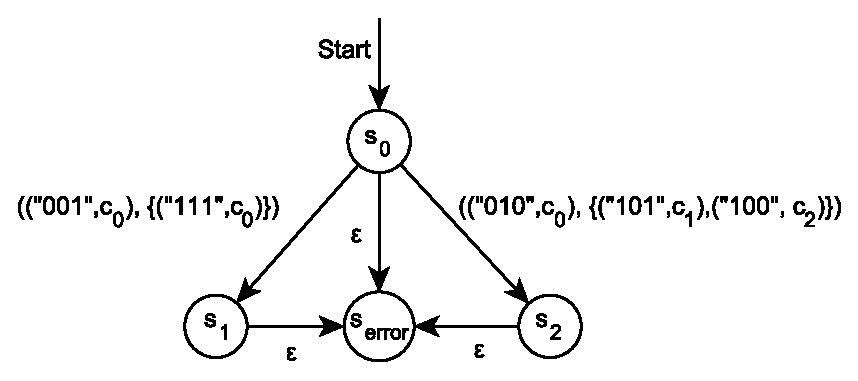
\includegraphics[scale=0.6]{figures/state-machines/simple-NFA.pdf}
		\caption{A simple example of our finite state machine model\label{fig:simple-nfa}}
	\end{figure}

	To show the transformation, we will model an arbitrary distributed protocol as consisting of \textit{finite state machines}, \textit{channels} and \textit{processes}.
	A finite state machine consists of a current state, $s_{current}$, a finite set of $n$ distinct states, $S=\{s_1, s_2, \dots, s_n\}$, and a finite set of $m$ distinct state-transitions, $T$.
	A finite state machine can only be in one state at any time, and transitions to another state by accepting a bit-vector as input, and optionally outputs another bit-vector.
	A transition has the form $(s_{from}, i, o, s_{to})$, where $i$ is an input consisting of a pair of a bit-vector and the channel the bit-vector was received on, and $o$ is the output consisting of a set of bit-vector/channel pairs, each representing that bit-vector being sent on the appertaining channel.
	For example, the finite state machine in Figure~\ref{fig:simple-nfa} will transition from the starting state $s_0$ to $s_2$ on input $"010"$ from channel $c_0$, and will during the transition output $"101"$ to channel $c_1$ and $"100"$ to $c_2$.

	A channel is bi-directional and can either be reliable or unreliable.
	A reliable channel guarantees that messages sent on it will be delivered in the order the messages were sent, and will not be changed during transmission.
	An unreliable channel gives no such guarantees, and can thus experience loss, reordering and corruption of messages.

	The last component in our model is the process.
	A process is a set of running state machines.
	The state machines inside the process can be connected with reliable channels.
	State machines can be connected to state machines in other processes only with unreliable channels.

	\begin{figure}[ht]
		\center
		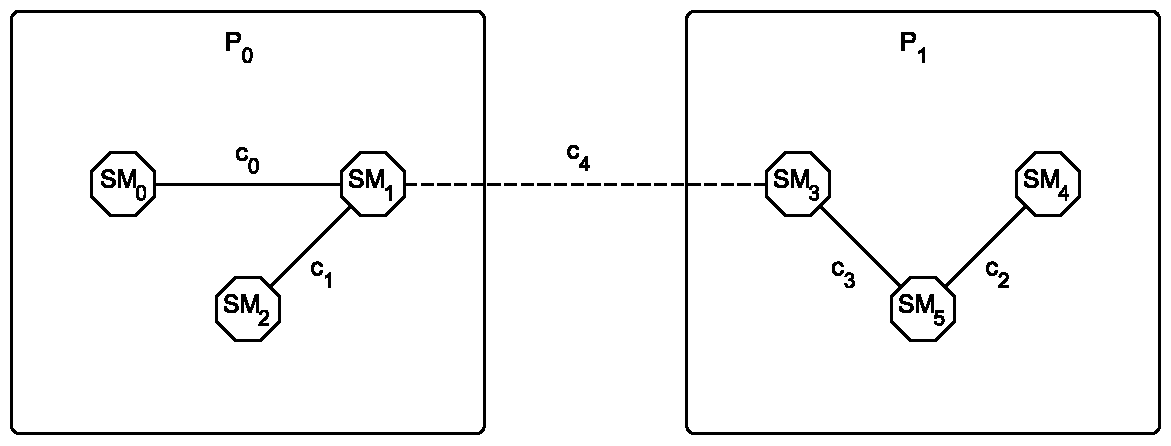
\includegraphics[scale=0.6]{figures/state-machines/Distributed-protocol-model.pdf}
		\caption{A simple example of distributed protocol model.\label{fig:simple-model}}
	\end{figure}

	Figure~\ref{fig:simple-model} is a model of a simple distributed protocol, consisting of the processes $P_0$ and $P_1$, each of which have three state machines $SM_0 - SM_5$.
	Each state machine is connected to other state machines on the same process with reliable channels $c_0-c_3$, and $SM_1$ on $P_0$ is connected to $SM_3$ on $P_1$ by the unreliable channel $c_4$.

	A distributed protocol can experience a number of different errors.
	Apart from the channel faults already described, we will model crashes and byzantine faults, as these are the ones we are concerned about in this transformation.
	We model a crash fault in the state machine by adding an empty input transition ($\epsilon$) from every state to an error-state, which cannot transition to any state (see $s_{error}$ in Figure~\ref{fig:simple-nfa}).
	As the state machine will not be able to transition to another state, and thus cannot output anything from this state, this serves to model a component crashing in a distributed protocol.
	We model a byzantine fault by exchanging a process with a new process.
	This potentially includes the removal of state machines, the addition of state machines or the exchange of old state machine with new state machines with new current states and new channels (we will refer to this last case as \textit{corrupted} state machines).
	This models a process exhibiting arbitrary behaviour.

	To transform a crash-resistant distributed protocol into a byzantine-fault-tolerant protocol, we utilize the verification in Remote Attestation (see Section~\ref{subsec:attestation}) and the integrity guarantees provided by Intel SGX.
	To model the integrity and confidentiality guarantees, we introduce the notion of a cryptographic secret state machine $SM_{s}$, and an integrity protected area of the process.
	We assume that any byzantine fault can replicate $SM_{s}$, but cannot replicate the secrets contained in $SM_s$, under a corruption of $SM_s$.
	This models that faulty processes cannot access the cryptographic secrets of a correct process, which is a reasonable assumption by the integrity and confidentiality guarantees given by Intel SGX, if the secrets are stored in an enclave (see Section~\ref{subsec:enclave}).
	State machines running in the integrity protected area of the process can be uniquely identified by $SM_{s}$, but cannot have channels to state machines running on other processes.
	This models the integrity protection in Intel SGX and abilities of the QE, as well as an enclave's inability to access peripheral hardware such as network cards.

	To model the Remote Attestation verification, we introduce a Remote Attestation process, $P_{RA}$ and an Attestation state machine, $P_A$, which will communicate with $P_{RA}$ to verify and provision $SM_s$ with a symmetric secret key.
	We will not go into detail with, or model, the Remote Attestation protocol in this section, as the specifics of it are inconsequential with regards to this transformation.
	For more information on the Remote Attestation protocol, see Section~\ref{subsec:attestation},~\cite{costan_intel_2016} and/or~\cite{intel_sgx_developer_reference}.

	We will also assume that each process has a unique identifier, $id_p$, that $SM_s$ knows $id_p$, and that each untransformed state machine includes both this $id_p$ and the $id_p$ of the intended receiver in its outgoing messages.
	In the case of broadcast messages, the $id_p$ of the receiving processes can be omitted.
	In practise, this could be implemented as a process's external IP-address that is provisioned to $SM_s$ by in a verifiable or trusted manner (for instance by $P_{RA}$ during secret provisioning), or by a sufficiently large number that is randomly selected on process start up.
	Both of these solutions require a handshake protocol during channel establishment, in which $SM_s$ on each process must MAC their $id_p$ with the Remote Attestation provisioned secret for verification by the other process.
	We will not describe this handshake protocol.

	The transformation of a crash-resistant protocol to a byzantine-fault-tolerant protocol consists of 4 steps on the process-level:
	\begin{enumerate}
		\item Add all the state machines to the integrity protected area of the process.
		This is equivalent to making the distributed components in the crash-resistant protocol into enclaves.
		Please note that it is rarely necessary to guarantee integrity for all components.
		Instead the minimal necessary number of components, the TCB, should be identified and protected.
		For the general case, however, every component is part of the TCB.
		\item For each endpoint state machine in unreliable channels between processes, add a new state machine in the unprotected area of each of the processes (called a wrapper state machine), connect a new unreliable channel between these and add a reliable channel from the old endpoint state machines to the new.
		This is equivalent to adding unprotected wrapper components for the enclaves, which will have access to the network, and thus can act as a middle-man for communicating with other processes.
		\item Add reliable channels from all state machines in the integrity protected area of the process to the cryptographic secret state machine $SM_s$.
		\item Add an Attestation state machines, $SM_A$, to each process and a Remote Attestation process, $P_{RA}$ to the protocol.
	\end{enumerate}

	\begin{figure}[ht!]
		\center
		\includegraphics[scale=0.40]{figures/state-machines/distributed-protocol-model-transformation0.pdf}
	\end{figure}
	\begin{figure}[ht!]
		\center
		\includegraphics[scale=0.40]{figures/state-machines/distributed-protocol-model-transformation1.pdf}
	\end{figure}
	\begin{figure}[ht!]
		\center
		\includegraphics[scale=0.40]{figures/state-machines/distributed-protocol-model-transformation2.pdf}
	\end{figure}
	\begin{figure}[ht!]
		\center
		\includegraphics[scale=0.40]{figures/state-machines/distributed-protocol-model-transformation3.pdf}
	\end{figure}
	\begin{figure}[ht!]
		\center
		\includegraphics[scale=0.40]{figures/state-machines/distributed-protocol-model-transformation4.pdf}
		\caption{Transformation of Figure~\ref{fig:simple-model} from crash-resistant protocol to byzantine fault-tolerant protocol.}
		\label{fig:tranformation-model}
	\end{figure}
	\FloatBarrier

	The transformation of the state machines consists of the following:
	\begin{enumerate}
		\item Before a process runs the protocol, a pre-compute step must be added where each process' $SM_s$ is provisioned with the same cryptographic secret.
		This is handled by the $SM_s$ and $SM_A$, which will contact $P_{RA}$ and be Attested and securely provisioned.
		In our example, we have only added a single $P_{RA}$, which of course means that a \textit{k}-resilient protocol suddenly cannot handle a single $P_{RA}$ crash.
		This can be solved by adding \textit{k+1} identical $P_{RA}$s, as this is a pre-compute step.
		This means that the $P_{RA}$s plays no further role after this step in the protocol, and can crash without effecting the running processes.
		\item All messages that were to be sent in the original protocol, must be sent from a state machine in the integrity protected area though a state machine in the unprotected area of the process.
		This is due to the constraint that the state machines in the integrity protected area of the process can no longer have channels to other processes.
		\item Before any message intended for another process is sent from the integrity protected area, it must have a cryptographic message authentication code (MAC) appended to the message.
		The MAC is an output of the message and the key provisioned with Remote Attestation.
		$SM_s$ is the only state machine with the Remote Attestation provisioned key, and thus only $SM_s$ can MAC a message correctly.
		$SM_s$ will refuse to sign any message if any state machine in the integrity protected area is not the original.
		This translates to a transformation of the state machine, such that each transition $(s_{from}, i, \{(m_o, c_o)\}, s_{to})$, where $c_o$ is a channel that was previously to another process, must be transformed to the transitions $(s_{from}, i, \{(m_o, c_{SM_s})\}, s_{wait})$ and $(s_{wait}, (m_o+MAC, c_{SM_s}), \{(m_o+MAC, c_o)\}, s_{to})$ with the intermediate state $s_{wait}$, which acts as a state in which the state machine waits for $SM_s$ to MAC the output message.
		\item Whenever a message that supposedly originates from another process is received from the unprotected area by a state machine in the integrity protected area, the MAC of that message must be verified by $SM_s$.
		In case this verification fails, the message must be discarded.
		This translates to a transformation of the state machine, such that each transition $(s_{from}, (m_i, c_i), o, s_{to})$, where $c_i$ is a channel that was previously to another process, must be transformed to the transitions $(s_{from}, (m_i+MAC, c_i), \{(m_i+MAC, c_{SM_s})\}, s_{wait})$, $(s_{wait}, ("0", c_{SM_s}), \{\}, s_{from})$ and  $(s_{wait}, ("1", c_{SM_s}), o, s_{to})$ with the intermediate state $s_{wait}$, which acts as a state in which the state machine waits for $SM_s$ to verify the MAC of the input, and the messages $"0"$ and $"1"$ represents the failure and success of this verification, respectively.
		\item In the event that $SM_s$ is asked to sign a message from a state machine that it identifies is not the original state machines in the integrity protected area, it must discard the message.
	\end{enumerate}

	Notice that this transformation is linear in the number of messages, under the assumption that the MAC, and MAC-verification sub-routines in $SM_s$ do not add any messages.
	Each input message in the transitions is transformed to exactly one new state, three new state transitions and one MAC-verification sub-routine on $SM_s$.
	Each output-set is transformed to exactly one new state, two new state transitions and $n$ MAC sub-routines on $SM_s$ where $n$ is the size of the output set.

	\begin{table}[ht!]
	\centering
	\makebox[\textwidth][c]{\begin{tabular}{r|l}
	\textbf{Msgs.}     & \textbf{Origin} \\ \hline
	$m$                             &  MAC-request outputs to $SM_s$.                                   \\ \hline
	$m$                             &  MAC-response inputs from $SM_s$.                                 \\ \hline
	$m$                             &  sending to the wrapper state machine on the sending process.     \\ \hline
	$m$                             &  sending between processes.                                       \\ \hline
	$m$                             &  sending from the wrapper state machine on the receiving process 	\\ \hline
	$m$                             &  input MAC verification requests to $SM_s$.                       \\ \hline
	$m$                             &  verification responses from $SM_s$.                              \\ \hline\hline
	$7\cdot m$                      &  total messages
	\end{tabular}}
	\caption{Number of messages after the transformation}
	\label{tab:number-of-messages-transformed}
	\end{table}

	Under the assumption that $SM_s$ sends no additional messages during the MAC and MAC-verification sub-routines, and no failures, $m$ messages in the original state machine will become $7m$ messages after the transformation (see table~\ref{tab:number-of-messages-transformed}).
	If we only count the messages sent between processes, there is no change in the number of messages sent.

	\FloatBarrier
	\begin{figure}[ht!]
		\center
		\makebox[\textwidth][c]{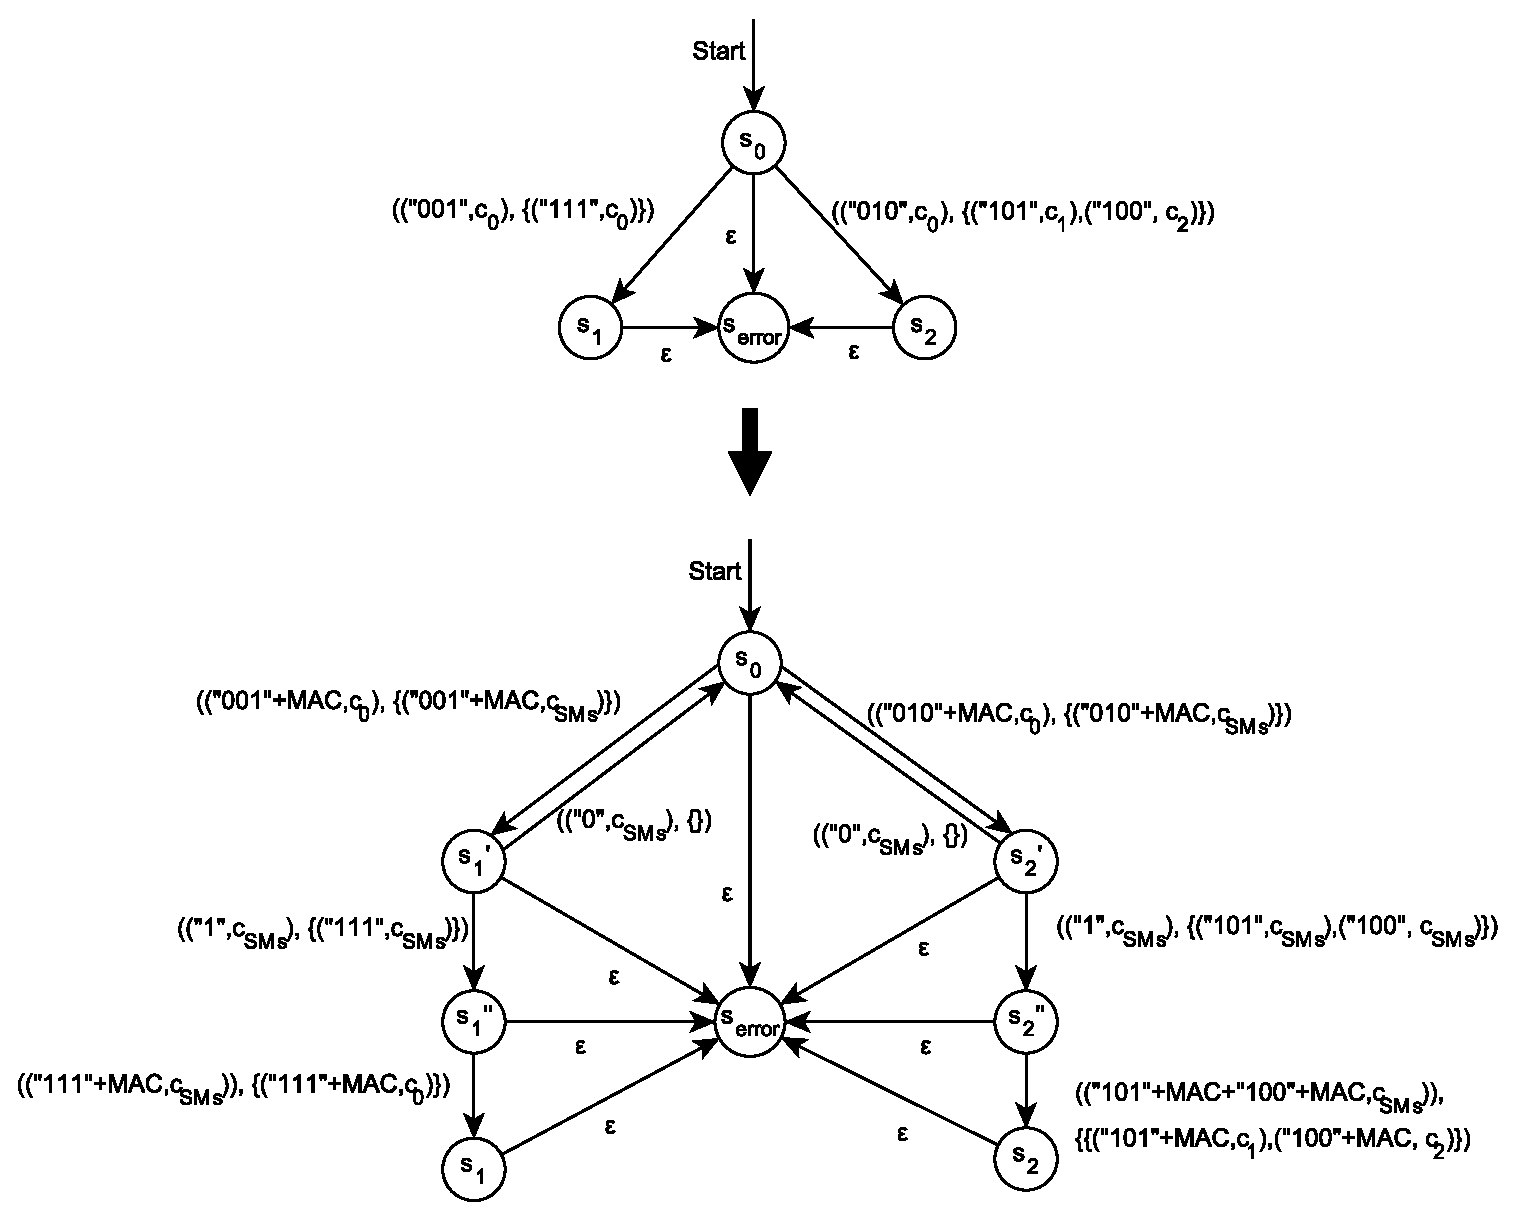
\includegraphics[scale=0.6]{figures/state-machines/NFA-transformation.pdf}}
		\caption{Transformation of Figure~\ref{fig:simple-nfa} from state machine in crash-resistant protocol to integrity protected state machine in byzantine fault-tolerant protocol, if all channels are to other processes.}
		\label{fig:nfa-transformation}
	\end{figure}
	\FloatBarrier

	These transformations gives us the following guarantees, relevant if a process experiences a byzantine fault.
	Recall that we model a byzantine fault as a process being exchanged with a new process, potentially with removed, added and/or corrupted state machines.
	\begin{itemize}
		\item If a process has its transformed state machine removed, the process will exhibit exactly the same behaviour as a crash (the state machine can take no further inputs, and produce no further outputs), and so it is exactly equivalent to a crash of the state machine.
		\item If the wrapper state machines are removed, the transformed state machine can no longer send or receive messages.
		This is again equivalent to a crash, as a token can no longer be sent to or from that state machine.
		\item If the $SM_A$ is removed, it can either happen before or after the Remote Attestation process has completed:
		\begin{itemize}
			\item If it happens before, the process's $SM_S$ will never be provisioned with the Remotely Attestation secret, and no messages will be verified.
			Therefore, the transformed state will never have its outgoing messages MAC'ed nor will it have any incoming messages verified.
			As such, it will either get stuck in a state where it never gets a response from $SM_s$ of a message MAC request, or it will get stuck in a state where a specific message cannot be verified.
			\item If it happens after the provisioning it will have no effect, as $SM_s$ is already provisioned, and no further communication with $SM_A$ is required.
		\end{itemize}
		\item If a process gets an additional state machine in the integrity protected area, it will have no consequence, as $SM_s$ will refuse MAC'ing and verification of messages from this state machine, and it cannot communicate with other state machines, unless these are corrupted.
		\item If a process gets an additional state machine outside the integrity protected area, it cannot communicate with anything inside the integrity protected area, with corrupting these (see below).
		It can communicate with other non-protected state machines, but this is equivalent to the other state machines being corrupted (see below).
		\item If a process has a corrupted transformed state machine (in the integrity protected area), $SM_s$ will refuse to sign any messages.
		So any messages sent from this corrupted state machine, will not be verified on correct processes, meaning that the transformed state machines receiving this message will not transition any further than the verification state.
		\item If a process has a corrupted $SM_s$, the new $SM_s$ will not have access to the Attestation secret.
		Therefore, it cannot MAC or verify messages.
		Nor can it be provisioned with the key again, as this the Remote Attestation procedure ensures that $SM_s$ is the correct state machine.
		\item If a process has a corrupted wrapper state machine, any messages from the integrity protected area can either be dropped, changed/corrupted, redirected, or duplicated:
		\begin{itemize}
			\item A dropped message is equivalent to a dropped message on an unreliable channel, which the protocol already handles.
			\item A corrupted message will not be verified by a correct receiving process's $SM_s$, and the message will be discarded.
			\item A redirected message will be not by verified by the receiving process, as it's $id_p$ will not match the intended recipient, and the message will be discarded.
			\item A duplicated message is equivalent to a duplicated message on the unreliable channel, which the protocol already handles.
		\end{itemize}
	\end{itemize}

	This concludes the argument that Intel SGX and cryptography can change the behaviour of correct process under byzantine faults to behaviour equivalent to that of crash faults, and thereby, using the above transformation, make a crash-resistant protocol into a byzantine fault tolerant protocol.
	As we will apply this transformation to our solution, we will from here on in, only consider a fault model of crashing processes.

		\subsection{Example: Central Server Mutual Exclusion}

		We will now show a practical example of how the transformation in Section~\ref{sec:transforming-byzantine-faults} can be applied.
		The protocol that we will transform is the central server protocol for mutual exclusion (CSME).
		The central server protocol for mutual exclusion is a protocol which partly solves the \textit{distributed mutual exclusion} problem.
		In the distributed mutual exclusion (ME) problem, a collection of processes share one or more resources (referred to as the \textit{critical section}), and need to perform reads/writes on these resources.
		To prevent race-conditions, a mutual exclusion algorithm ensures that only a single process has access to the critical section at any given time.
		More formally, in any solution to the distributed mutual exclusion problem, the following requirements must be upheld:
		\begin{description}
			\item[ME1: Safety] At most one process may execute in the critical section (CS) at a time.
			\item[ME2: Liveness] Requests to enter and exit the critical section eventually succeed.
		\end{description}
		Optionally, some distributed mutual exclusion protocols also solves the additional fairness requirement of
		\begin{description}
			\item[ME3: Happened-before ordering] If one request to enter the CS happened-before another, then entry to the CS is granted in that order.
		\end{description}
		CSME solves ME1 and ME2 under the conditions of no process failures.
		However, CSME does not fulfil the requirements of ME3 in asynchronous systems, and thus only partly solves the distributed mutual exclusion problem.

		In broad strokes, the protocol works by deploying a central server process, which will process a request for access to the critical section in the received order, send an access token to the appropriate client process, wait for an acknowledgement from the process that access to the critical section is no longer needed, and then process the next request.
		It is trivial that the protocol does not provide liveness under process crashes | if the server crashes, no process can gain access tokens, and thus no requests for access will succeed.
		The same scenario is true if a process crashes while having access to the critical section, as the server will never release the token of the crashed process.
		However, safety is still guaranteed, as a process cannot access the critical section without a token.
		Under byzantine faults, neither safety nor liveness can be guaranteed.
		For instance, the server could serve the tokens to all requests without waiting for acknowledgements from the clients.

		We will now show how the transformation from Section~\ref{sec:transforming-byzantine-faults}, can transform CSME to give the same guarantees in a byzantine system as the untransformed protocol gives in a crash-fault system.
		Note that there is no formal definition of how the critical section access and token is implemented in CSME | it can be implemented with cryptography, as partial states, with append-only memory, as another process, etc.
		We will keep this abstraction in the following transformation, but the implementation of this is also required to undergo the same transformation.
		We will omit the handling of unreliable channels on the state machines for readability, but assume that it is handled.

		First we need to model the protocol as finite state machines, channels and processes.
		We model two different state machines: a client state machine, and a server state machine.

		\FloatBarrier
		\begin{figure}[ht!]
			\center
			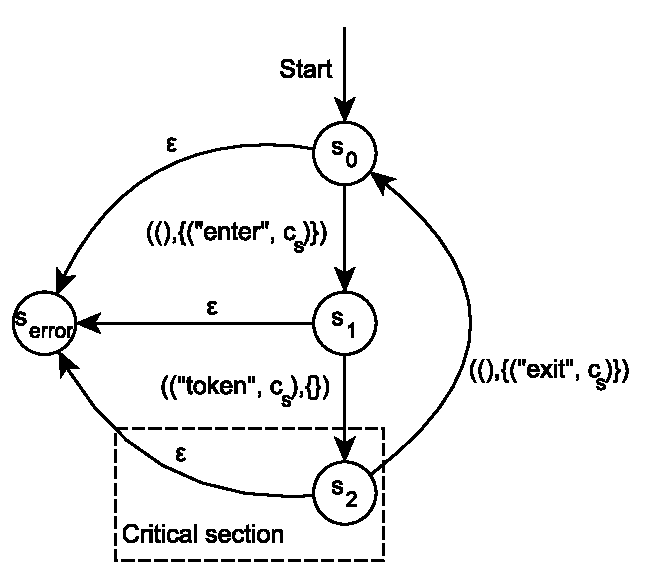
\includegraphics[scale=0.6]{figures/state-machines/CSME-client-NFA.pdf}
			\caption{Client state machine from the central server protocol for mutual exclusion. Note that the channel $c_s$ represents the unreliable channel to the server, and is different across client instances.}
			\label{fig:CSME-client-NFA}
		\end{figure}
		\FloatBarrier

		The client state machine is modelled in Figure~\ref{fig:CSME-client-NFA}.
		It can either not have requested access to the critical section ($s_0$), wait for the token from the server ($s_1$), or have the token and be in the critical section ($s_2$).
		Naturally it can also crash ($s_{error}$).

		\FloatBarrier
		\begin{figure}[ht!]
			\center
			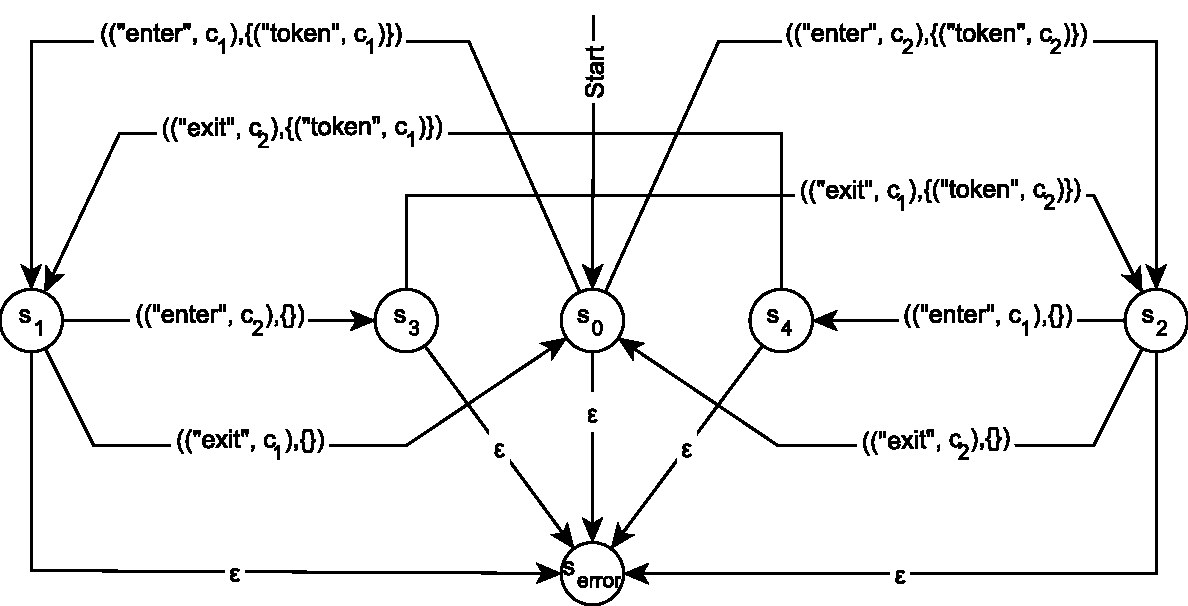
\includegraphics[width=\textwidth]{figures/state-machines/CSME-server-NFA.pdf}
			\caption{Server state machine from the central server protocol for mutual exclusion. Note that this server state machine can only handle two client processes.}
			\label{fig:CSME-server-NFA}
		\end{figure}
		\FloatBarrier

		The server state machine is a bit more complex as it must be modelled to account for the number of client processes.
		Figure~\ref{fig:CSME-server-NFA} is a model of the server state machine in a protocol with two client processes.
		It encompasses 6 states:
		\begin{description}
			\item[$s_0$] where no client has access to the critical section, and no requests have been sent.
			\item[$s_1$] where no client has access to the critical section and client $1$ has requested the token and the token has been sent.
			\item[$s_2$] where no client has access to the critical section and client $2$ has requested the token and the token has been sent.
			\item[$s_3$] where client $1$ has the token and client $2$ has requested the token.
			\item[$s_4$] where client $2$ has the token and client $1$ has requested the token.
			\item[$s_{error}$] where the state machine has crashed.
		\end{description}

		\FloatBarrier
		\begin{figure}[ht!]
			\center
			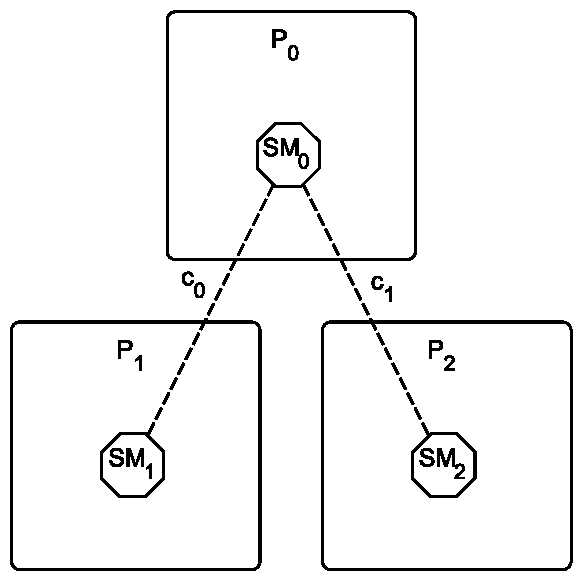
\includegraphics[scale=0.6]{figures/state-machines/CSME-protocol.pdf}
			\caption{Processes and channels in the central server protocol for mutual exclusion, with one server and two clients.}
			\label{fig:CSME-protocol}
		\end{figure}
		\FloatBarrier

		Figure~\ref{fig:CSME-protocol} shows the processes and channels in CSME with two client processes.
		$P_1$ and $P_2$ are the clients, each running an instance of the state machine from Figure~\ref{fig:CSME-client-NFA}, with an unreliable channel to the server process $P_0$, which runs an instance of the state machine from Figure~\ref{fig:CSME-server-NFA}.

		We start the transformation by transforming the state machines to have their messages MAC'ed by $SM_s$, and to have $SM_s$ verify the messages they receive.
		This is done by applying the state machine replication transformation described in Section~\ref{sec:transforming-byzantine-faults}.

		\FloatBarrier
		\begin{figure}[ht!]
			\center
			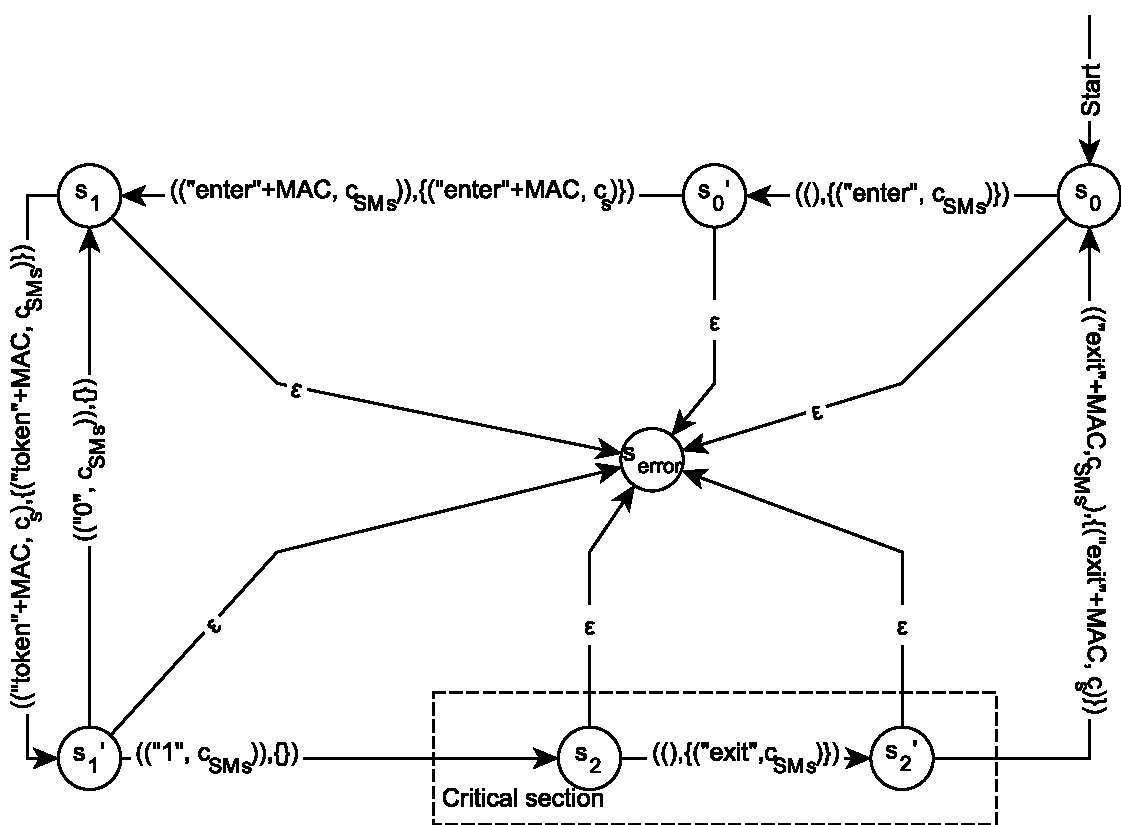
\includegraphics[width=\textwidth]{figures/state-machines/CSME-client-NFA-transformed.pdf}
			\caption{Client state machine in CSME, after it has been transformed to handle byzantine faults.}
			\label{fig:CSME-client-NFA-transformed}
		\end{figure}
		\FloatBarrier

		Figure~\ref{fig:CSME-client-NFA-transformed} shows the client state machine after the transformation.
		Whenever the client wants to enter the critical section, the state machine sends the request to $SM_s$ for MAC'ing.
		When the MAC'ed message is received from $SM_s$, this message is sent to the server process.
		The state machine is now in $s_1$, which is equivalent to $s_1$ in the untransformed state machine (Figure~\ref{fig:CSME-client-NFA}).
		$c_s$ is now a channel from the wrapper state machine.
		When a token is received from $c_s$, the message's MAC is sent to $SM_s$ for verification.
		If the MAC is correct, the state machine will transition to $s_2$, which is in the critical section, and is equivalent to $s_2$ in the untransformed state machine.
		Before exiting the critical section, the exit message is sent to $SM_s$ for MAC'ing, and when the appropriate MAC is received from $SM_s$, the exit message is sent to the wrapper state machine for redirection to the server process.

		\FloatBarrier
		\begin{figure}[ht!]
			\center
			\makebox[\textwidth][c]{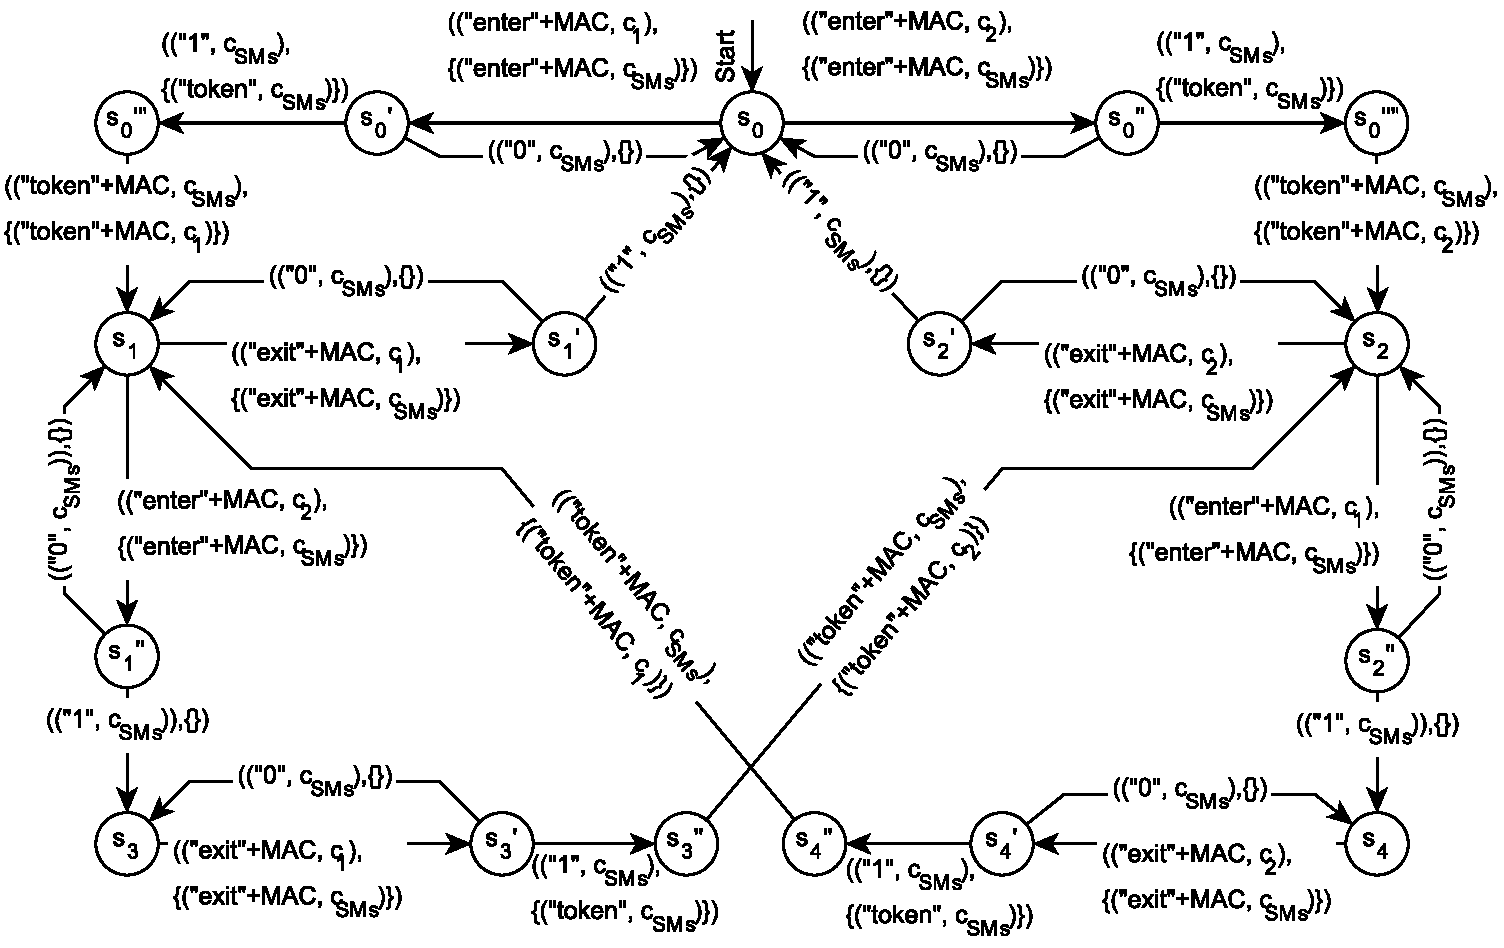
\includegraphics[width=\textwidth]{figures/state-machines/CSME-server-NFA-transformed.pdf}}
			\caption{Server state machine in the central server protocol for mutual exclusion, after it has been transformed to handle byzantine errors. Note that $s_{error}$ has been omitted for improved readability.}
			\label{fig:CSME-server-NFA-transformed}
		\end{figure}
		\FloatBarrier

		Figure~\ref{fig:CSME-server-NFA-transformed} shows the transformed server state machine.
		We have omitted $s_{error}$ for readability.
		$s_0$, $s_1$, $s_2$, $s_3$ and $s_4$ are equivalent to the states by the same names in the untransformed state machine (Figure~\ref{fig:CSME-server-NFA}).

		\begin{description}
			\item[$s_0$] the token has been released, and no client has requested the token.
			\item[$s_1$] client $1$ has requested the token, $SM_s$ has verified the MAC of the request and MAC'ed the token which has then been sent to the servers wrapper state machine for redirection to the client $1$ process.
			If the token is released by client $1$, and this message's MAC is verified, the state machine will transition to $s_0$.
			\item[$s_2$] is equivalent to $s_1$, except with client $2$ instead of client $1$.
			\item[$s_3$] client $1$ has the token, and client $2$ has requested the token.
			So when the server state machine receives an "exit" message verifiably from client $1$, a token is MAC'ed and sent to client $2$, so the state machine can transition to $s_2$.
			\item[$s_4$] is equivalent to $s_3$, except with the clients reversed (client $2$ has the token, client $1$ has requested it, when client $2$ releases the token).
		\end{description}

		\FloatBarrier
		\begin{figure}[ht!]
			\center
			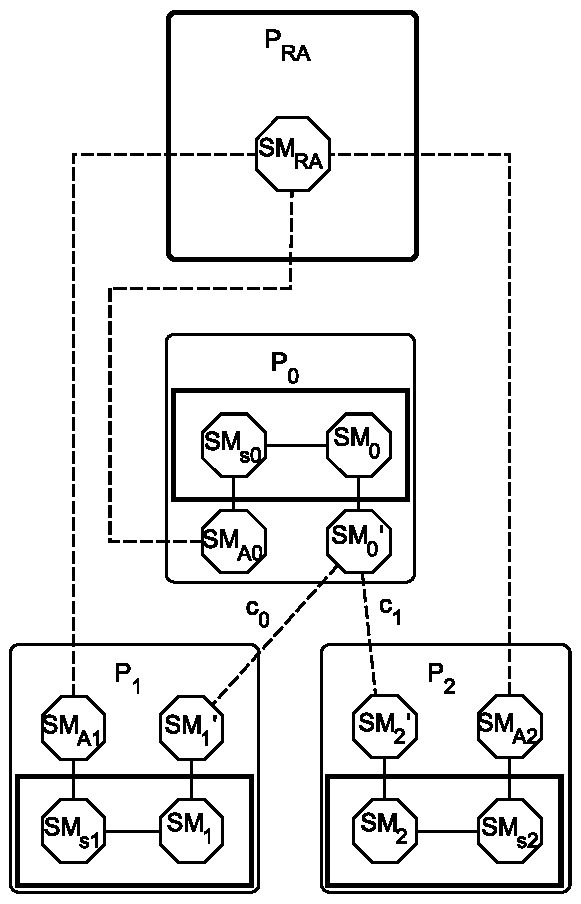
\includegraphics[scale=0.6]{figures/state-machines/CSME-protocol-transformed.pdf}
			\caption{Processes and channels in the central server protocol for mutual exclusion, after they have been transformed to handle byzantine errors.}
			\label{fig:CSME-protocol-transformed}
		\end{figure}
		\FloatBarrier

		Figure~\ref{fig:CSME-protocol-transformed} show the process's transformation.
		Each of the client processes ($P_1$ and $P_2$), is now running the transformed client state machines in the integrity protected area.
		The transformed client state machines have a reliable channel to a $SM_s$, and another to a wrapper state machine outside the integrity protected area, which is responsible for passing on the messages to the server process.
		Each of the processes have a $SM_A$ responsible for passing Remote Attestation messages from the $SM_s$ to the new Remote Attestation process.
		The server process is running a transformed server state machine, connected to two wrapper state machines and an $SM_s$.
		The server $SM_s$ is also connected to a $SM_A$ for attestation.

		Having transformed the CSME protocol, the correct processes will exhibit the same behaviour when other processes suffer byzantine faults, as the correct processes do in the untransformed protocol when other processes suffer crash faults.

		\FloatBarrier
		\begin{figure}[ht!]
			\center
			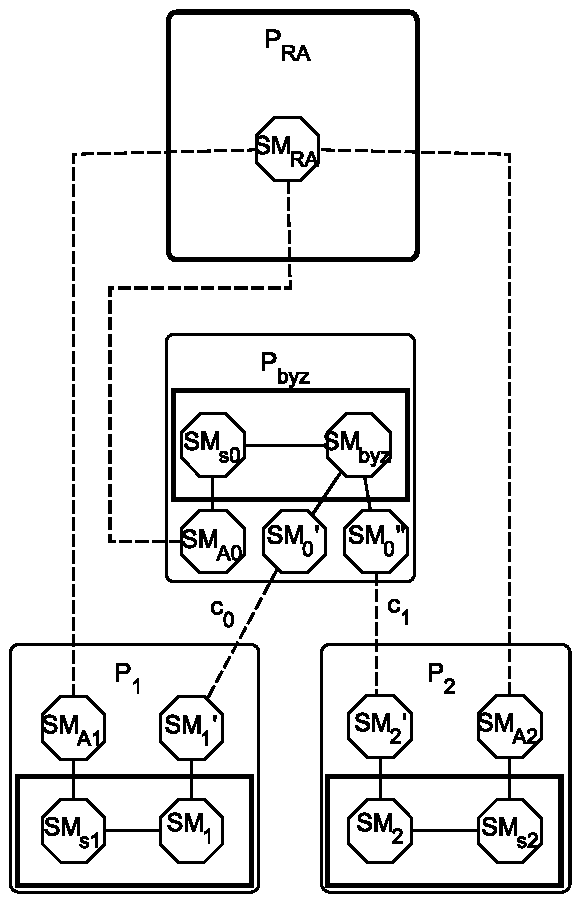
\includegraphics[scale=0.6]{figures/state-machines/CSME-protocol-transformed-byzantine.pdf}
			\caption{Processes and channels in the transformed central server protocol for mutual exclusion, with a byzantine fault on the server process.}
			\label{fig:CSME-protocol-transformed-byzantine}
		\end{figure}
		\FloatBarrier

		As an example, consider a situation where the server state machines tries to serve tokens on any request, without getting acknowledgement that the token has been released by the client who last held the token.
		There are several ways this could be modelled, one of which is presented here:
		We model this byzantine fault as $P_0$ being exchanged with $P_{byz}$.
		$P_{byz}$ (see Figure~\ref{fig:CSME-protocol-transformed-byzantine}) is exactly equal to $P_0$, except that $SM_0$ has been exchanged with $SM_{byz}$ (see Figure~\ref{fig:CSME-server-NFA-transformed-byzantine}), which serves a token to any request by the clients.

		\FloatBarrier
		\begin{figure}[ht!]
			\center
			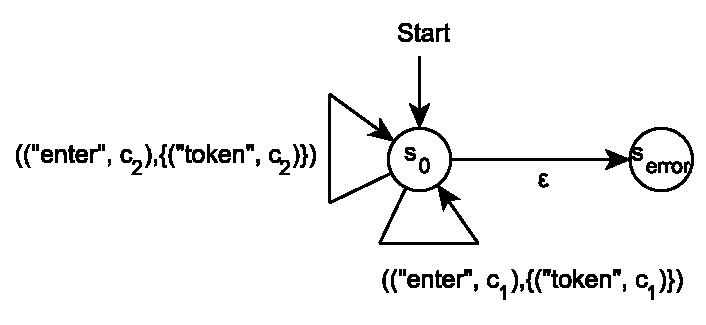
\includegraphics[scale=0.6]{figures/state-machines/CSME-server-NFA-transformed-byzantine.pdf}
			\caption{The byzantine fault state machine $SM_{byz}$ on the server process.\label{fig:CSME-server-NFA-transformed-byzantine}}
		\end{figure}
		\FloatBarrier

		If this byzantine fault happens, none of the tokens are MAC'ed.
		Thereby, any correct client process (Figure~\ref{fig:CSME-client-NFA-transformed}) will get stuck in a loop between $s_1$ and $s_1'$, when $SM_s$ rejects the token as it has not been MAC'ed.
		This is equivalent behaviour to the server process crashing, as a token will never be accepted, and the client is unable to enter the critical section.

	\section{Analysis}
	\label{sec:analysis}

	With a better understanding of the prerequisite information, we now present a more thorough definition of the problem.

	We define our system as having $n$ peers $\{p_1, p_2 \dots p_n\}$, and a DCR graph $G$, which consists of $v$ events $E = \{e_1, e_2, \dots, e_v\}$ and a set of relations between events, $R$.
	Each peer is said to be \textit{responsible} for one or more events, where being responsible for an event, $e$, means that requests for executions of $e$ and requests for the state of $e$ can be handled by that peer.
	Furthermore the system must have the following properties:
	\begin{description}
		\item[Safety] all peers responsible for $e$ execute the requests on $e$ in the same order.
		\item[Liveness] The client of a request eventually receives a reply to that request.
		\item[DCR linearisability] At any time before and after event executions, the states of $e_1, e_2, \dots, e_v$ must be the result of at least one run $R_G$ of $G$. Recall that $R_G$ only contains all successful executions.
	\end{description}

    Recall that we wish to create a system which is:
    \begin{description}
        \item[Concurrent] Simultaneous execution of concurrent events, as defined in Section~\ref{subsubsec:concurrency}, is performed without requiring that those executions are synchronised in the system.
        \item[Scalable] Achieving consensus is done in less than $O(n)$ messages, where $n$ is the number of peers in the graph, while supporting the distribution of the state of the DCR graph among the participants.
        \item[Byzantine fault tolerant] Byzantine behaviour is detectable, through the guarantees provided by Intel SGX, and treated as crashes.
    \end{description}

	 Additionally, any peer should be able to collect the run, $R$, which is compatible with all prior collected runs, meaning that a run collected at logical time $t$, must be prefixed by a run equivalent up to concurrency, to a run collected at time $t-1$.
     Note that from this, it follows that two runs collected at time $t$, are not required to be identical, but are required to be equivalent up to concurrency, as defined in~\ref{subsubsec:concurrency}.
     Since the peers responsible for each event can always be required to store executions which it has \textit{observed} and include it alongside the state of the event, we assume that collecting a run will always be possible, as long as maintaining the state of the graph is and therefore disregard it at this point in the analysis, and return to it in Section~\ref{subsec:global-history-collection}.

	\begin{landscape}
		\begin{table}
		\centering
		\makebox[\textwidth][c]{\begin{tabular}{ p{4cm} p{1.5cm} p{1.5cm} p{1.5cm} p{1.5cm} p{2cm} p{2.3cm} p{2cm} }
		\toprule
		\textbf{Approach}		  			& \textbf{FT: Availability}    			& \textbf{FT: Safety} & \textbf{FT: Data integrity} & \textbf{Crash recovery} 	& \textbf{Minimum complexity for executing $e$} 	& \textbf{Concurrency}      	& \textbf{Request Bottleneck}\\
	    \midrule
		Central Server 			  			& $0$                                   & $n$                 & $0$                         & n/a                       & $2$                                       		& $\leq$ Dynamic independence 	& $1$ \\
		State Machine Replication 			& $\lfloor \frac{(n-1)}{2} \rfloor$     & $n$                 & $n-1$                       & $O(n)$                    & $2\cdot\lfloor\frac{(n-1)}{2}\rfloor$     		& $\leq$ Dynamic independence 	& $1$ \\
		Partial state, single-leader 		& $\lfloor \frac{(m-1)}{2} \rfloor^*$ 	& $n$                 & $m-1$                       & $O(n^2)$                  & $2\cdot\lfloor\frac{(m-1)}{2}\rfloor$     		& Dynamic independence 			& $1$ \\
		Complete distribution 				& $0^*$                               	& $n$                 & $0$                         & n/a                       & $2\cdot D_{dyn}(G,e)$           					& Dynamic independence 			& $n$ \\
		Partial state, multi-leader 		& $\lfloor \frac{(m-1)}{2} \rfloor^*$ 	& $n$                 & $m-1$                       & $O(m)$                    & $2\cdot\lfloor\frac{(m-1)}{2}\rfloor$     		& Dynamic independence 			& $\frac{n}{m}$ \\
		\bottomrule
		\end{tabular}}

		\caption[caption]{Comparison of different approaches to solving the problem. $^*$ denotes partial availability loss. \textbf{FT: Availability} is the fault tolerance of the availability guarantee. \textbf{FT: Safety} is the fault tolerance of the safety guarantee. \textbf{FT: Data integrity} is the fault tolerance of data integrity. \textbf{Crash recovery} is the number of messages required to recover from a crashing process. \textbf{Minimum complexity for executing $e$} is the minimum number of messages needed for the execution of an event. \textbf{Concurrency} is the supported level of DCR concurrency. \textbf{Request Bottleneck} is how many processes' can handle execution requests at one time.}
		\label{tab:approach-comparison}
		\end{table}
	\end{landscape}

	We consider several possible approaches to solving this problem, the performance of which can be seen in Table~\ref{tab:approach-comparison}.
	The following is a short summary of each approach starting at the most intuitive, followed by iterative improvements of it:

    \FloatBarrier
    \begin{figure}[ht!]
        \center
        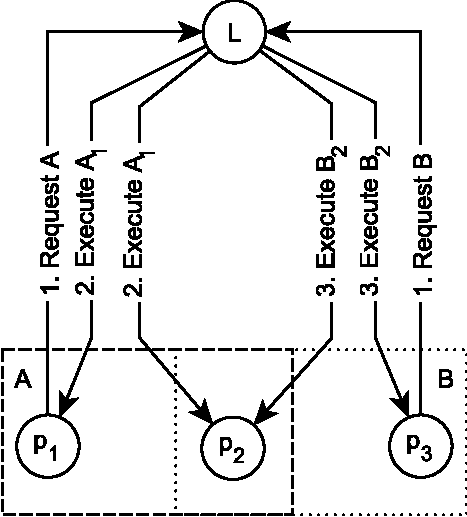
\includegraphics[scale=0.7]{figures/dcr-graphs/central-server-approach}
        \caption{The central server approach.
        The messages are ordered by the leader, $L$, such that the execution of $A$ is applied before the execution of $B$.
        Note that the executions are numbered in the logical order which they are sent.
        Peer $p_1$ is responsible for event $A$ along with $p_2$.
        Peer $p_3$ is responsible for event $B$ along with $p_3$.}
        \label{fig:central-server-approach}
    \end{figure}
    \FloatBarrier

	\paragraph{Central server approach}
	The first approach is a simple central server.
    An example of the simultaneous execution of two events, $A$ and $B$, are shown in Figure~\ref{fig:central-server-approach}.
	There is a single leader, $L$, each of the other peers replicate some subset of $E$ and can redirect requests to the leader.
	When the leader receives a request, it is queued in the order they are received, and applied to $G$ in that order.
	After the execution of an event $e$, each of the peers replicating $e$ or an event in $E_{eff}(G,e)$ are informed by $L$ of that execution, with a counter value that enables ordering of the execution of the events.
	This ensures safety, since each of the peers will apply the executions in the same order as $L$.
	Since every request is managed by a single leader, we are automatically given DCR linearisability, since the executions are totally ordered.
	However, this solution does not ensure concurrency, since $L$ needs to apply each previous execution before the next.
	If concurrency is desired, $L$ can execute requests in parallel, while keeping track of current executions.
	When an execution request is received of an event that is dynamically dependent on one of the currently executing events, it is queued, and so is all other requests that are not in the approximate static independence set of all the currently executing and queued events.
	Furthermore, there is no fault tolerance because under a leader crash, there is no guarantee that the remaining peers can recreate the most recent state.

    \FloatBarrier
    \begin{figure}[ht!]
        \center
        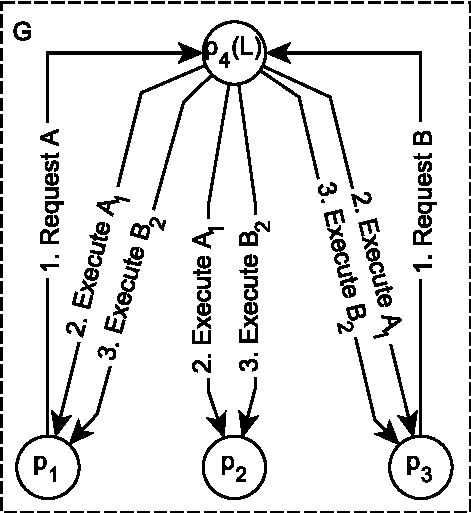
\includegraphics[scale=0.7]{figures/dcr-graphs/smr-approach.pdf}
        \caption{The SMR approach.
        Following the same semantics as in Figure~\ref{fig:central-server-approach}, with the exception that each peer is responsible for the entire graph.}
        \label{fig:smr-approach}
    \end{figure}
    \FloatBarrier

	\paragraph{SMR approach}
	The next approach tries to improve on the fault tolerance of the central server approach.
    An example of the simultaneous execution of two events, $A$ and $B$, is shown in Figure~\ref{fig:smr-approach}.
	This is a classic SMR/consensus solution with crash fault tolerance.
	There are several protocols that solve the issue of SMR, for instance in~\cite{bracha_asynchronous_1985,lamport_part-time_1998,lamport_lower_2006,ongaro_search_2014}, but as they are largely interchangeable with regards to performance\footnote{In the categories specified in the Table~\ref{tab:approach-comparison}.}, any solution that utilizes a leader, $L$, to achieve an optimal crash fault tolerance of $f = \lfloor \frac{(n-1)}{2} \rfloor$ is enough.

	In this approach, every peer must replicate all events, as all executions must be committed to at least $f+1$ replicas.
	This ensures that if a leader dies, a new leader can be chosen (using $O(n)$ messages), which gives us the aforementioned fault tolerance.
	However, now $L$ must synchronise all requests, to ensure that they are applied in the same order by all replicas, which translates to no concurrency in executions.
	Some SMR protocols (e.g.~\cite{castro_practical_1999}) allow for concurrent request commits, under the constraint that requests that are committed must not be applied to the underlying state machine before any uncommitted request that happened-before~\cite{lamport_time_1978} on $L$.
	In order to allow for the concurrent execution of dynamically independent events, this constraint could be relaxed to allow for applying the execution of $e$ when the request has committed, if the peer is aware of which events is in the previous uncommitted execution requests, and none of these events are in $D_{dyn}(e)$.
	Because the peer needs to know the previous uncommitted requests, this results in worse concurrency than dynamic independence.
	Furthermore, the solution still needs $O(n)$ messages to execute a single event, no matter how the graph is constructed.

    \FloatBarrier
    \begin{figure}[ht!]
        \center
        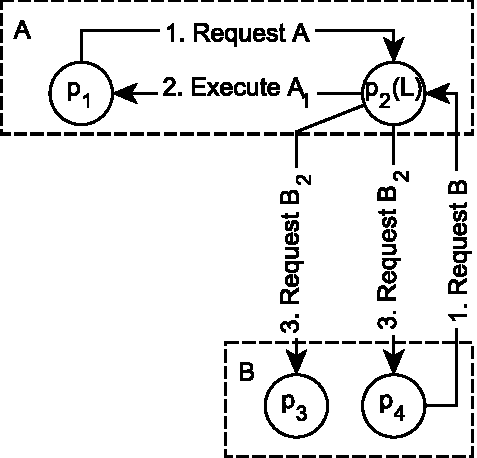
\includegraphics[scale=0.7]{figures/dcr-graphs/partial-state-single-leader-approach.pdf}
        \caption{The partial state, single leader approach.
        There are two clusters, one for event $A$ containing $p_1$ and $p_2$, and one for event $B$ containing $p_3$ and $p_4$.
        The leader is currently $p_2$.}
        \label{fig:partial-state-single-leader-approach}
    \end{figure}
    \FloatBarrier

	\paragraph{Partial state, single leader approach}
	The next approach is an attempt to reduce the amount of messages needed for executing an event.
    An example of the simultaneous execution of two events, $A$ and $B$, is shown in Figure~\ref{fig:partial-state-single-leader-approach}.
	The basic idea is to distribute the event responsibility out to a subset of peers, which will then only be responsible for that event.
	We name these subsets \textit{clusters} and denote the size of these clusters $m$.
	The system still utilizes a single leader, which synchronises the requests.
	When event $e$ is requested executed, the leader runs an SMR algorithm similar to the one described in the SMR approach, but only with the cluster for $e$, and the clusters of $E_{eff}(G,e)$ | to ensure that the clusters of $E_{eff}(G,e)$ has updated the state/enabledness of the events they are responsible for.
	This ensures a lower message complexity than the SMR approach, given $n > m \cdot (|E_{eff}(G,e)|+1)$ where $n$ is the number of peers in the system.
	Notice that $\forall e. n = m \cdot v \geq m \cdot (|E_{eff}(G,e)|+1))$ where $v$ is the number of events in the graph.
	And for sufficiently loosely connected graphs where no event's execution affect all other events in the graph, $\forall e. n > m \cdot (|E_{eff}(G,e)|+1))$.
	Another improvement is the fact that if more than half of a cluster crashes, only part of the availability is affected, since the statically independent clusters can continue operating normally.
	However, $L$ must still synchronise all requests, and worse, cannot allow for concurrent request commits, since the peers would not necessarily be able to recreate the synchronisation between these.
	The one exception is dynamically independent events, since the ordering of the execution of these does not matter.
	Under leader crashes, all clusters need to synchronise their logs, which would require $O(n^2)$ messages.

    \FloatBarrier
    \begin{figure}[ht!]
        \center
        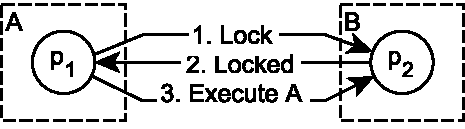
\includegraphics[scale=0.7]{figures/dcr-graphs/complete-distribution-approach.pdf}
        \caption{The complete distribution approach.
        Note that the executions are no longer numbered, as synchronisation is done using locks.}
        \label{fig:complete-distribution-approach}
    \end{figure}
    \FloatBarrier

	\paragraph{Complete distribution approach}
	The next approach is heavily inspired by~\cite{hildebrandt_safe_2011}.
    An example showing the execution of an event is shown in Figure~\ref{fig:complete-distribution-approach}.
	In it $n = v$, and each peer is only responsible for a single event.
	There is no leader, and an execution is done through synchronisation between peers.
	If event $e$ is to be executed, the responsible peer will use a synchronisation technique (e.g. 2 phase locking~\cite{skeen_nonblocking_1981}) with all the peers responsible for the events in $E_{eff}(G,e)$, who will update their state accordingly.
	This guarantees DCR linearisability.
	The fault tolerance of this approach is quite poor, as any peer crashing will result in a data loss, and effect availability, even though it has the same property as the partial state, single leader approach of not effecting the events in $I_{stat}(e)$.

    \FloatBarrier
    \begin{figure}[ht!]
        \center
        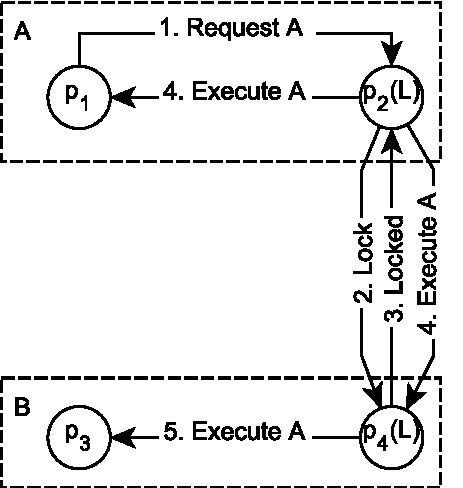
\includegraphics[scale=0.6]{figures/dcr-graphs/partial-state-multi-leader-approach.pdf}
        \caption{The partial state, multi leader approach.
        Note that this example is in a graph where events $A$ and $B$ are not dynamically independent, meaning that synchronisation is required.
        Furthermore, locking is not the only way to achieve synchronisation and it is only used as an example here. }
        \label{fig:partial-state-multi-leader-approach}
    \end{figure}
    \FloatBarrier

	\paragraph{Partial state, multi-leader approach}
	The last is our chosen approach, and we will go into detail with it from Section~\ref{subsec:algorithm}.
    An example showing the execution of an event is shown in Figure~\ref{fig:partial-state-multi-leader-approach}.
	It is built upon the partial state, single leader approach, except that the common leader is replaced with inter-cluster synchronisation using locks.
	This has the benefit that even if a leader dies, the recovery has message complexity $O(m)$ (instead of $O(n^2)$ in the partial state, single leader approach and $O(n)$ in the SMR approach), and the number of concurrent client requests are not bounded by the processing speed of a single process.
	From here on in, we will primarily concern ourselves with the details of the partial state, multi-leader approach.

	\subsection{Algorithm}
	\label{subsec:algorithm}

	To avoid the high number of messages associated with a fully replicated system and the message bottleneck associated with a single-leader system, we propose a multi-leader, partial state system.
	Each event is represented by an individual leader, who can initiate execution of that event at any given time.
	Since events can affect each other and this system is in an asynchronous setting where messages can be delayed arbitrarily, having multiple leaders can potentially lead to situations where leaders disagree on which order events have been executed in, possibly resulting in disagreement on the state of the workflow.
	The semantics for discerning when ordering is needed and how that ordering is applied is described in Section~\ref{subsec:execution-ordering}.

	Given a method of ordering event executions, ensuring that the system can sustain faults means that each event needs to not only be stored by a leader, but rather a number of peers, called a \textit{cluster}, one of which is the leader at any given time.
	Clusters being responsible for events rather than single peers means that executions and locks need to be synchronized for each individual cluster.
	Due to the fact that these clusters can be seen as completely individual networks of peers, any consensus algorithm can be used to solve the problem of synchronizing executions and locks as it is completely detached from the locking mechanism and reduces to the problem of consensus.
	Choosing a consensus algorithm to manage the clusters is however still an important decision, as the wrong choice could form significant bottlenecks in the system.
	For this implementation we have chosen Raft~\cite{ongaro_search_2014}, as the basis for the cluster consensus algorithm, modified by the transformation we described earlier in Section~\ref{sec:transforming-byzantine-faults} to reduce byzantine faults to crash-stop failures.
	The reason for choosing Raft is that it is widely used commercially, relatively simple and able to achieve consensus in very few messages.
	Additionally Raft only handles crash faults and is therefore an ideal candidate for the transformation of byzantine faults to crashes.
	The consensus algorithm applied in the clusters is described in Section~\ref{subsec:cluster-consensus}.

	With the two parts described above, peers can now progress the graph, in the sense that events can be executed safely, but since each peer only knows the state of events which clusters it belongs to, what has transpired in the graph is implicitly distributed.
	Since the algorithm does at this point guarantees that any event can only execute, when the semantics and the state of the graph permits it, collecting the global history is only interesting from a documentation perspective.
	Suppose that a node which is only a member of clusters of events which are never executed, that node will have no way of knowing if anything in the graph is being executed at all.
	Additionally, it is useful to know the entire history of the graph, when evaluating whether or not the graph has served its purpose.
	For these reasons, we present the \textit{CheapShot} algorithm for collecting the global history of a DCR graph in Section~\ref{subsec:global-history-collection}.

	\subsection{Execution Ordering}
	\label{subsec:execution-ordering}

	For this section, we apply terms used in directed graphs and define variations of neighbourhoods with regards to DCR graphs as:
	\begin{description}
		\item[Out-neighbourhood] denoted $N_{out}(e)$, defined as the set of events where event $e'$ is in $N_{out}(e)$ iff there is a relation in $G$ that originates from $e$ and targets $e'$.
		\item[In-neighbourhood] denoted $N_{in}(e)$, defined as the set of events where event $e'$ is in $N_{in}(e)$ iff there is a relation in $G$ that originates from $e'$ and targets $e$.
	\end{description}

	As discussed in Section~\ref{sec:analysis}, the execution of non-independent events must be synchronised.
	The need for ordering executions is applicable in cases where two or more executions would have incompatible effects on at least one event.
	As ordering must necessarily be detrimental to the concurrency of a DCR graph and must also require some amount of communication between events, minimizing the situations where ordering is required is a priority.
	Recall the definitions from Section~\ref{subsubsec:concurrency}, where the dependencies in DCR graphs are explained, and realize that dynamic independence so far describes the cases where ordering is not needed.
	This means that the cases where ordering is needed would seem to be defined by \textit{dynamic dependence}, meaning cases where for two events, $e_1$ and $e_2$, it holds that $E(E(G, e_1),e_2) \neq E(E(G, e_2),e_1)$.
	There is however a small caveat to this, illustrated by the following example:

	Consider a graph consisting of two events with a condition between them: $\ev{A} \crel \ev{B}$
	Events \texttt{A} and \texttt{B} are dynamically dependent, as executing first \texttt{A} and then \texttt{B} results in a different graph than executing first \texttt{B} and then \texttt{A}, since \texttt{B} cannot be executed in the latter case.
	According to the goal of preventing dynamically dependent events from executing simultaneously, an execution of event \texttt{A} would require ordering on both \texttt{A} and \texttt{B}.
	This is unnecessary as it is impossible for event \texttt{B} to execute before event \texttt{A} has been either executed or excluded.
	Both of the constraints share this property and since constraints furthermore do not modify states, there is no need for \texttt{A} to ensure ordering of its execution on \texttt{B} or indeed for any event to ensure ordering of its execution on events which it is targeting only with a constraint.

	\begin{figure}[ht!]
		\center
		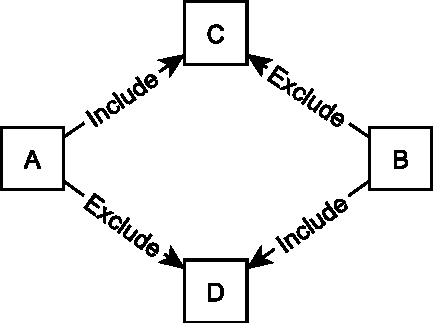
\includegraphics[scale=0.5]{figures/dcr-graphs/race-condition.pdf}
		\caption{Graph illustrating the need for ordering effects in $N_{out}(e)$.}
		\label{fig:race-condition}
	\end{figure}

	If \texttt{A} has effects originating from it, the need for synchronization arises as shown in Figure~\ref{fig:race-condition}.
	In the graph events \texttt{A} and \texttt{B} both modify the same event state attributes and a race condition is present as a result.
	In order to prevent the race condition from having adverse effect, synchronization is needed between the two executing events, \texttt{A} and \texttt{B}.
	This means that events with effects which target events within $N_{out}(E)$ need to ensure synchronisation on the targeted events of $e$'s execution.

	Since effects can modify events which in turn have constraints originating from it, there are situations where locking in the neighbourhood of the executed event is no longer sufficient.

	\begin{figure}[ht!]
		\center
		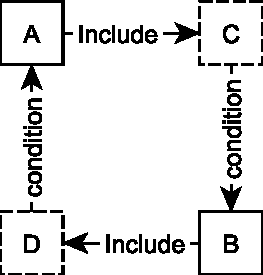
\includegraphics[scale=0.5]{figures/dcr-graphs/second-degree-effect.pdf}
		\caption{Graph illustrating that ordering only within $N_{out}(e) \cup e$ is insufficient.}
		\label{fig:second-degree-effect}
	\end{figure}

	In the graph shown in Figure~\ref{fig:second-degree-effect} it is shown that the set of events requiring ordering of an execution has to include either a subset of $N_{out}(N_{out}(e))$, $N_{in}(e) \cup N_{out}(e)$ or $N_{in}(N_{in}(e))$.
	Otherwise, the graph could end in a state where only \texttt{A} and \texttt{B} have been executed, which should be impossible due to the execution of either including a condition on the other.
	As ordering within the set of $N_{in}(N_{in}(e))$ is not enough on its own, due to the case shown in Figure~\ref{fig:race-condition}, we regard this option as worse than any of the other two.

	We now show that the cases shown in Figure~\ref{fig:race-condition} and in Figure~\ref{fig:second-degree-effect} cover all situations where ordering is needed.
	According to the semantics of DCR relations (see Section~\ref{subsec:dcr}), the enabledness of an event, $e$, can only be changed by state changes in $N_{in}(e) \cup e$, and the state of the event can only be affected by an execution in $N_{in}(e) \cup e$.
	Consider an event $e$.
	Executing $e$ can then change the state and enabledness of any event in $N_{out}(e) \cup e$.
	Changes of the enabledness of an event in $N_{out}(e)$ cannot propagate\footnote{Unless the enabledness change of the event is a result of a state change of the event, e.g. if the event is excluded}, since no relation relies on the enabledness of the originating event.
	Changes of the state of an event in $N_{out}(e)$, \textit{can} propagate, since the constraining relations relies on the state of the originating event.
	But since only the constraining relations rely on the state of the originating event, the state change can only propagate enabledness changes, which in turn cannot propagate.

	Summarized we have the following cases where ordering must occur:
	\begin{description}
		\item[Effect] Consider a graph of two events: \ev{A} and \ev{B}, with an effect originating from \texttt{A}, targeting \texttt{B}.
		If \texttt{A} is executed, ordering of that execution must be ensured on \texttt{B}.
		\item[Effect-Condition] Consider a graph of three events: \ev{A}, \ev{B} and \ev{C}, with an effect originating from \texttt{A}, targeting \texttt{B} and a constraint originating from \texttt{B}, targeting \texttt{C}.
		If \texttt{A} is executed, ordering of that execution must be ensured on \texttt{B} and \texttt{C}.
	\end{description}
	Both of these cases can be covered by ordering in $N_{out}(N_{out}(e)) \cup N_{out}(e) \cup e$ or $N_{in}(e) \cup N_{out}(e) \cup e$.

	\begin{figure}[ht!]
		\center
		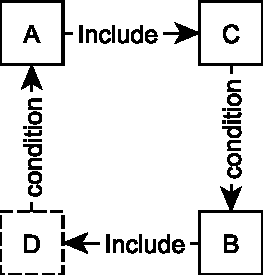
\includegraphics[scale=0.5]{figures/dcr-graphs/second-degree-no-effect.pdf}
		\caption{Graph illustrating the advantage of locking in $N_{out}(N_{out}(e)) \cup N_{out}(e) \cup e$ rather than $N_{in}(e) \cup N_{out}(e) \cup e$.}
		\label{fig:second-degree-no-effect}
	\end{figure}

	In the graph shown in Figure~\ref{fig:second-degree-no-effect} an execution of \texttt{A} no longer has an effect on the enabledness of \texttt{B}, as \texttt{C} is included and therefore has the same state before and after the execution of \texttt{A}.
	An argument can be made here for the $N_{out}(N_{out}(e)) \cup N_{out}(e) \cup e$ ordering scheme over $N_{in}(e) \cup N_{out}(e) \cup e$, as it allows for optimizations in that ordering is not needed on \texttt{B}, meaning that the former ordering scheme would be more efficient than the latter.
	This optimization is, however, only possible when the state of \texttt{C} is known and this is not a trivial problem.
	The solution of simply notifying \texttt{A} of \texttt{C}'s state when changed, is insufficient as the notification might not arrive before \texttt{A} performs ordering based on a previous state.
	A different solution could be to evaluate the need for ordering in steps, meaning that in the described example, \texttt{A} would inform \texttt{B} that it is executing and that ordering is required and \texttt{B} then evaluates whether or not ordering on \texttt{C} is needed, based on the state of \texttt{B}.
	This two-step solution has the disadvantage of potentially taking twice as long, assuming that transporting a message between \texttt{A} and \texttt{C} takes the same amount of time as between \texttt{A} and \texttt{B}.

	There are additionally three cases where the ordering scheme described so far is not maximally concurrent:
	\begin{itemize}
		\item $\ev{A} \erel \ev{B}, \ev{C} \erel \ev{B}$ When \texttt{A} is executing, it ensures ordering on \texttt{B}.
        If \texttt{C} then attempts to execute it will need ensure synchronisation on \texttt{B} as well.
        As the execution of \texttt{A} and \texttt{C} have exactly the same effects on \texttt{B}, the synchronisation of these two executions is inconsequential, as they are dynamically independent.
		\item $\ev{A} \irel \ev{B}, \ev{C} \erel \ev{B}$ When \texttt{A} is executing, it needs to ensure synchronisation on \texttt{B}.
        If \texttt{C} attempts to execute, it is clear that it must ensure synchronisation on \texttt{B} as well, however, \texttt{B} should be allowed to execute at any time, as it is dynamically independent with \texttt{A}.
        This is because the effect which the execution \texttt{A} has on \texttt{B} is not incompatible with the effects of an execution of \texttt{B} and the execution of \texttt{A} does not change the enabledness of \texttt{B}.
		\item $\ev{A} \irel \ev[100]{B}, \ev[100]{B} \crel \ev{C}$ When \texttt{A} is executing, it will need to ensure synchronisation on both \texttt{B} and \texttt{C} due to the constraint originating from \texttt{B} and targeting \texttt{C}.
        This is not needed, as the condition relation is invalidated by the fact that \texttt{B} is executed.
	\end{itemize}

    \subsubsection{Synchronisation Method}
    \label{subsubsec:synchronisation-method}

	Now that the cases where ordering is needed have been exhaustively described, as shown in~\cite{debois_concurrency_2015}, the actual method for synchronisation executions must be chosen.
	Synchronisation can be assured in a number of ways, but following from the goals specified for this solution, there are some that are a better fit than others.
	Consider an optimistic ordering system where events requiring synchronisation are notified of the execution and provided that no incompatible executions are performed simultaneously, that execution is considered committed.
	If incompatible executions are performed concurrently, however, the execution is discarded.
	This means that there is a period of uncertainty with regards to a execution, but as any peer needs to be able to obtain a run of a graph, which will be compatible with any future run collected, this optimistic method of ordering executions seems less than ideal.
	We therefore ideally need a way to be certain that an execution is possible before it is performed on any event.
	One way to accomplish this in reasonable time, is by using \textit{locking}.

	In a graph, $G(E,V)$, we define the set of locked events, $L$, on the execution of an event, $e$, as $L(e)$.
	An event can only be locked by a single event at any time and is unlocked when a lock either leads to an execution or when an execution is aborted due to all locks not being attainable.

	For the implementation described in this thesis, the simpler rules of ordering is implemented, namely always locking on \textbf{Effects} and on \textbf{Effect-Conditions} as described earlier, which should be sufficient as it covers all situations where synchronisation is needed.
	Furthermore, all locking is performed by the executing event, as we postulate that the costs of an additional round-trip is considerably more expensive in practice, than a redundant lock.

	\subsection{Global history collection}
	\label{subsec:global-history-collection}

	We define a global history to be a DCR run.
	Both as documentation of the process upon completion of the workflow and during the life cycle of the workflow, the global history is relevant, in the latter case because the global state can be derived from the global history.
	In this section we conflate a cluster with the event which the cluster is responsible for, for brevity.

	For a global history to be collectible, each event must track more than just their own executions, as the only relationships between executions that can be established are those that are observed locally on a single execution.
	Events must also track all executions that affect its state and enabledness.
	As locked events are implicitly notified of an execution upon unlocking, tracking these are trivial.
	There are, however, cases where locking is not performed but where enabledness is affected, as locking is concerned with preventing race conditions and not necessarily changes in enabledness.
	One such case is $\ev{A} \crel \ev{B}$, where \texttt{B} cannot execute before \texttt{A} is executed or excluded.
	In addition to locking, events in which enabledness is affected by an execution must therefore also be informed about that execution.

	It is assumed that informing events is attempted until the informed event responds.
	Under this assumption, an arbitrary amount of time can pass before an event is actually notified, but as this does not allow executions to happen which violate the semantics of DCR; it is reduced to a question of fairness, which will not be discussed in this thesis\footnote{Fairness in the sense that two events which enabledness is affected by an execution will not necessarily be notified of that execution at the same time, thereby allowing one event to execute before the other.}.

	A way to represent the state of a continuous system in an asynchronous setting is by finding a consistent cut~\cite{lamport_time_1978}, which is defined by the happened-before relations:

	\begin{description}
		\item[Happened-before 1 (HB1)] Process events occurring on the same process can be ordered in happened-before relations.
		\item[Happened-before 2 (HB2)] There is a happened-before relation between the sending and the reception of a message.
		\item[Happened-before 3 (HB3)] Happened-before relations are transitive.
	\end{description}

	A consistent cut requires that all process events obey the happened-before rules within the cut, meaning:
	\begin{itemize}
		\item If a process event, \textit{a}, happened-before another process event, \textit{b}, and \textit{b} is included in the cut, then so is \textit{a}.
		\item If a message is received within the cut, the sending of that message must also be within the cut.
	\end{itemize}

	One way to achieve a consistent cut, is to implement Chandra and Lamport's Snapshot algorithm~\cite{chandy_distributed_1985}.
	This would require incorporation of the snapshot algorithm into the consensus algorithm applied it each individual cluster, significantly increasing its complexity.
	Additionally, the snapshot algorithm requires flooding of the entire network, which results in $O(r)$  messages, where $r$ is the number of relations in the DCR graph.
	Instead, we present an alternative solution, where the client requiring the global history requests the execution log from each event cluster.
	The algorithm we present for collecting the global history, does so without locking or pausing the network and in $O(e)$ messages, where $e$ is the number of events in the DCR graph.
	As a consistent cut only makes sense in connected graphs, it holds that $v = e-1$ in the case where $v$ is minimal, but as each event can have one of each relation type to each event in the graph, $v$ can maximally be $v = 5\cdot e^2$, meaning that the message complexity of the proposed solution is significantly better than that of Chandra and Lamport's Snapshot algorithm, since the proposed solution would always require $O(e)$ messages.
	There is, however, considerations in that each event will then have their individual perceived sequence of executions, which might be dissimilar due to arbitrary message delays.
	After receiving an answer from each cluster, the client is able to merge the local executions sequences into a consistent cut, using the following algorithm.

	Given the observed executions of each event in the DCR graph, it is always possible to reduce the cut until consistency is at some point attained.
	In happened-before terms, an execution being committed locally and another event being notified of that execution, corresponds to sending a message (committing locally) and it being received (committing externally).
	Therefore if any event observes the execution of another event and that execution is not present in the sequence returned by the latter event, it must be disregarded from the cut as it violates HB2.
	Since this could lead to violation of HB1, each execution recorded after the disregarded execution is also disregarded.

	Consider a simple graph of two events with a condition between them: $\ev{A} \crel \ev{B}$.
	A global history collection is started, by a client requesting it from every cluster, and assume that \texttt{A} is the first event to send its execution sequence $\{\}$, after which \texttt{A} executes.
	Following \texttt{A}'s execution, \texttt{B} has been enabled, and upon receiving this information, \texttt{B} executes.
	\texttt{B} then receives the execution sequence request and responds with a sequence of $\{\texttt{A}, \texttt{B}\}$.
	In this specific example, nothing is lost by event \texttt{A}'s returned execution sequence not including the execution of \texttt{A}, as all executions are observed by \texttt{B}.
	However, if \texttt{A} is not executable, it is impossible to interpolate what has happened.
	An example of this is the graph $\ev{A} \erel \ev{B} \crel \ev{C} \crel \ev{D}$, where the collection of the global history could return an empty sequence for \texttt{A}, \texttt{B} and \texttt{C}, but a sequence of $\{\texttt{C}, \texttt{D}\}$ from \texttt{D}.
	It is unknown whether an execution of \text{A} or an execution of \texttt{B} allowed the execution of \texttt{C} and then \texttt{D}.
	To solve this, any execution not present in the sequence returned by the event itself is considered invalid and therefore that execution is deleted from the sequence of all events, as well as all following executions in that sequence.
	In the above example, this would mean that the execution of \texttt{B} in the history of \texttt{C} would be deleted, along with the execution of \texttt{C} as the execution of \texttt{B} happened-before the execution of \texttt{A}.
	The reason for this procedure is that if these executions are not omitted, a consistent cut is no longer guaranteed.

	\begin{figure}[ht!]
		\center
		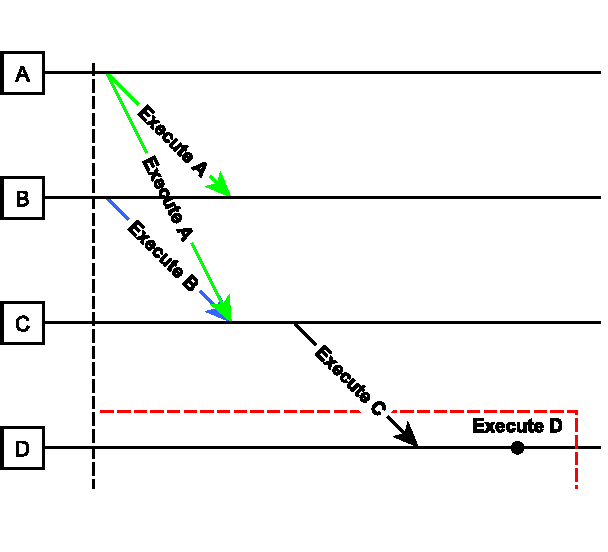
\includegraphics[scale=0.6]{figures/dcr-graphs/global-history-collection-consistent-cut.pdf}
		\caption{Global history collection consistent cut. Note that execution process of locking and then committing is illustrated as a single message, for brevity. The green and blue executions illustrate two possibilities which could have preceded \texttt{D}'s perceived execution sequence of $\{\texttt{C}, \texttt{D}\}$. The red, dotted line shows an inconsistent cut and the black, dotted line shows the found consistent cut.}
		\label{fig:global-history-collection-consistent-cut}
	\end{figure}
    \FloatBarrier

	In Figure~\ref{fig:global-history-collection-consistent-cut} the example from above is shown.
	As a consistent cut requires that any message received within the cut must also be sent within the cut (HB2), it is clear that the cut described in the figure is inconsistent.
	The method of carving an inconsistent cut described earlier, is the equivalent of ignoring that \texttt{D}'s cluster has received an execution message from \texttt{C}, which also renders the execution of \texttt{D} invalid.
	Cuts made in a DCR graph adhering to the tracking rules outlined here, and the implicit tracking of locks, will always be locally consistent, meaning that they are guaranteed to uphold the first premise of happened-before relations (HB1), namely ordering of local process events.

	Given that these events will always present a sequence adhering to HB1, it will always be possible to find a consistent cut.
	This is trivially true, in that each event will always be able to present an empty sequence, as an example of a consistent cut.
	Additionally, there will always be a guaranteed consistent cut, defined by the first\footnote{In the logical, happened-before, sense of first.} event cluster to reply with its observed execution sequence, as it will always be the sequence ending at the earliest, according to either definition of earliest.

	For locked events, the executing events record the execution after having received all locks, and before informing the locked events that execution has been achieved.
	For non-locking constraints, there can only exist the cases where the executing event has recorded an execution, but the constrained event has not, or when both has recoded the execution.
	As such, execution is always recorded locally before externally.
	But having a cut with a locally recorded execution that has not been externally recorded does not violate HB2, as the consistent cut contains the sending of the message (recording locally) but not the received message (recording externally).
	As such, any locally recorded executions of the first-receiving event does not require any external records and any external executions recorded must already have been recorded on locally by their respective events.

	Note that dynamically independent activities can cause sequences apparently contradicting one another.
	For example, a graph of $\ev{A} \crel \ev{B}, \ev{A} \crel \ev{C}, \ev{D} \crel \ev{B}, \ev{D} \crel \ev{C}$ could, by executing \texttt{A} and \texttt{D} concurrently, cause events \texttt{B} and \texttt{C} to perceive execution sequences of $\{\texttt{A}, \texttt{D}\}$ and $\{\texttt{D}, \texttt{A}\}$ respectively.
	This would appear to violate HB1, but since an event is notified of another event's execution without locking, it should be seen as sent and received messages.
	When \texttt{A} executes, it sends a notification to \texttt{C} and notes it in its execution sequence.
	When \texttt{C} receives a notification it notes it in its execution sequence.
	Thereby HB1 is not violated, as the execution of \texttt{A} is represented by two different events, meaning that it is covered by HB2.

	Now that a consistent cut is guaranteed, a valid execution sequence then has to be interpolated.

	\begin{figure}[ht!]
		\center
		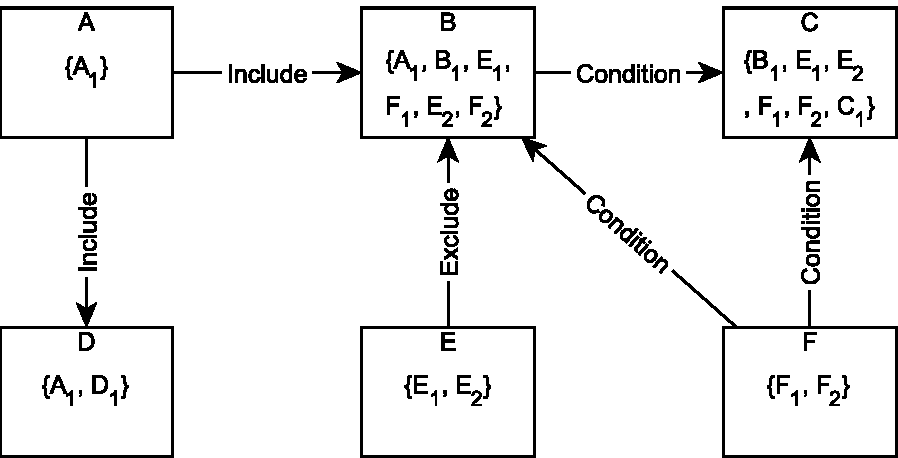
\includegraphics[scale=0.6]{figures/dcr-graphs/global-history-collection-example.pdf}
		\caption{Example graph illustrating global history collection. The sequences within a DCR event represent the execution sequence of that event.}
		\label{fig:global-history-collection-example}
	\end{figure}

	From the graph shown in Figure~\ref{fig:global-history-collection-example}, the shown sequences are returned by each respective event and form a consistent cut.
	Note that each execution of an event is uniquely identifiable by a tag, which is also the case in the algorithm described in this thesis, as it is needed by the cluster consensus part described in Section~\ref{subsec:cluster-consensus}.

	From each sequence, an implicit valid ordering is present, in the sense that from event \texttt{B} it is shown that execution $B_1$ can happen before $A_1$ happens.
	An linearisation of these sequences needs to be found, which can be accomplished through the construction of a directed graph and topologically ordering the vertices of that graph.
	Before a linearisation can be performed, we define each sequence as a set of execution relationships.
	For example the execution sequence recorded by \texttt{B} could also be formulated as: $\{A_1 \rightarrow B_1, B_1 \rightarrow E_1, E_1 \rightarrow F_1, F_1 \rightarrow E_2, E_2 \rightarrow F_2\}$ where the arrow denotes that the right hand side can occur after the left hand side, given that it has been observed.

	If each sequence is formulated as a series of execution relationships they can easily be aggregated in order to define the rules which a valid execution sequence must adhere to for this specific DCR graph and its state.
	For the example in Figure~\ref{fig:global-history-collection-example} where a union of the execution relationships result in the following set of relationships: $\{A_1 \rightarrow D_1, A_1 \rightarrow B_1, B_1 \rightarrow E_1, E_1 \rightarrow E_2, E_1 \rightarrow F_1, F_1 \rightarrow F_2, F_1 \rightarrow E_2, E_2 \rightarrow F_2, F_2 \rightarrow C_1\}$

	\begin{figure}[ht!]
		\center
		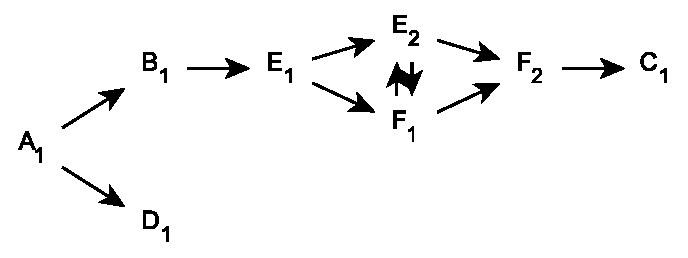
\includegraphics[scale=0.6]{figures/dcr-graphs/execution-sequence-graph-example.pdf}
		\caption{Initial graph made from sequence rule aggregation.}
		\label{fig:execution-sequence-graph-example}
	\end{figure}
    \FloatBarrier

	From the total list of relationships, a graph can now be constructed of possible executions, as seen in Figure~\ref{fig:execution-sequence-graph-example}.
	Because the execution of dynamically dependent events is not required to be synchronized, a cycle is present in that the relationship $F_1 \rightarrow E_2$ is present in the set as well as the, seemingly contradictory, $E_2 \rightarrow F_1$.
	This is still valid, as cycles in the happened-before relationships of executions, entails that the executions happened concurrently, because the locking rules would ensure an ordering if they were not independent.
	And since the locking rules from Section~\ref{subsec:execution-ordering}, only allow concurrent executions when the events are dynamically independent, any linearisation of the concurrent executions must result in the same state of the graph.
	Topological ordering behaviour with regards to cyclical graphs is, however, undefined and as cycles in the graphs created from execution relationships define concurrent executions, any ordering of executions in a cycle is valid.

	A topological ordering of event executions is obtained by performing a Depth-First Search (DFS), and returning its reverse postorder graph traversal.
	The DFS traversal is started at an arbitrary vertex.
	The vertex is marked as visited, and the DFS is continued in an unmarked neighbour.
	When a vertex is reached that has no unmarked neighbours, that vertex is prepended to the resulting linearisation.
	When the DFS has been run, we choose another unmarked arbitrary vertex and run the DFS from that vertex.
	Note that a reverse postorder DFS graph traversal is exactly a topological order, if the graph is a directed \textit{acyclic} graph~\cite[chapter 4, page 582]{sedgewick_algorithms_2011}.
	In order to extend the algorithm to allow any order of vertices in cyclical components, the third case of the proof is replaced with the following:
	\begin{itemize}
		\item The marked neighbour has been visited in the \textit{same} DFS traversal, implying that the two vertices are part of a cycle.
		But in this case, any ordering of the two vertices are acceptable, as it implies that the event executions, that the two vertices represent, happened concurrently.
	\end{itemize}
	Pseudo code of the DFS traversal algorithm can be seen in Listing~\ref{lst:dfs-traversal}.
\begin{snippet}
\begin{mdframed}[backgroundcolor=Papyrus]
	\begin{lstlisting}[style=pseudo, keywords={}]
L <- Empty list that will contain the sorted vertices
while there are unmarked nodes do
    select an unmarked node n
    visit(n)

 function visit(node n)
    if n is marked then return
    mark n
    for each node m with an edge from n to m do
        visit(m)
    add n to head of L
	\end{lstlisting}
\end{mdframed}
\caption{Reversed postorder DFS traversal algorithm. Adapted from~\cite{_topological_2018} \label{lst:dfs-traversal}.}
\end{snippet}

	There are four different steps to the process of collecting the execution history of a graph.
	\begin{enumerate}
		\item Collecting the perceived execution sequences of each event cluster.
		This requires $O(e)$ messages, where $e$ is the number of event clusters.
		\item Carving a consistent cut.
		This is accomplished by creating a look-up table which maps an execution to a set of all occurrences of that execution in returned sequences.
		For each of $m$ executions in each of $e$ returned sequences, the event which that execution pertains' returned sequence is checked for the presence of that execution.
		If an execution is deleted this way, it could have cascading effects.
		But under the assumptions that look-ups in the aforementioned table, as well as checking whether or not a sequence contains a specific execution, is constant, we can at most do this operation once for each execution entry in all sequences.
		For a graph with $e$ events and $m$ unique executions performed during the lifetime of the graph, this then has computational complexity of $O(e\cdot m)$.
		\item Creating a graph from execution relationships. As each relationship is represented with an edge, this has computational complexity of $O(n)$ where $n$ is the number of execution relationships.
		\item Finding a topological ordering.
		Using the DFS traversal algorithm, means visiting each node twice via its edges and therefore this operation has a computational complexity of $O(|r|+|e|)$, where $r$ is the number of relations in the graph and $e$ is the number of events in the graph.
	\end{enumerate}

	In conclusion the global history can be collected in $O(e)$ messages and within $O(e\cdot m)$ computational complexity, as finding a consistent cut forms the lower bound of the algorithm.

	\subsection{Cluster Consensus}
	\label{subsec:cluster-consensus}

	\begin{table}[ht!]
    	\centering
        	\makebox[\textwidth][c]{\begin{tabular}{l p{1.7cm} p{1.5cm} l p{1.7cm}}
            \toprule
        	\textbf{Algorithm} 								& \textbf{Fault tolerance (liveness)} & \textbf{Crash recovery} & \textbf{Messages/execution}  & \textbf{Fault tolerance} \\
            \midrule
        	PBFT~\cite{castro_practical_1999}               & $f = \lfloor \frac{n-1}{3} \rfloor$ & $(2f+1)^2$              & $(2f+1)+(2f+1)^2$            & Byzantine 				     \\
        	MinBFT~\cite{veronese_efficient_2013}           & $f = \lfloor \frac{n-1}{2} \rfloor$ & $(f+1)^2$               & $2(f+1)+(f+1)^2$             & Byzantine 				     \\
        	FastBFT~\cite{liu_scalable_2016}           		& $f = \lfloor \frac{n-1}{2} \rfloor$ & $(f+1)^2$               & $4(f+1)$                     & Byzantine 				     \\
        	Chandra-Toueg~\cite{chandra_unreliable_1996}    & $f = \lfloor \frac{n-1}{2} \rfloor$ & $0$                     & $4(f+1)+(f+1)^2$             & Crash                         \\
        	Paxos~\cite{lamport_part-time_1998}  			& $f = \lfloor \frac{n-1}{2} \rfloor$ & $0$                     & $4(f+1) + 2$                 & Crash                         \\
        	Raft~\cite{ongaro_search_2014}               	& $f = \lfloor \frac{n-1}{2} \rfloor$ & $2(f+1)$                & $2(f+1)$                     & Crash                         \\
            \bottomrule
        	\end{tabular}}
    	\caption{Comparison of different consensus algorithms}
    	\label{tab:comparison-consensus-algorithms}
	\end{table}

    Recall that the consensus algorithm applied in each cluster can be regarded separately from the rest of the algorithm, as locking a cluster or executing an event reduces to the problem of consensus.
	Each cluster therefore requires a SMR/consensus algorithm to achieve consensus on the state of their shared event.
	Table~\ref{tab:comparison-consensus-algorithms} shows a comparison between some classical SMR/consensus algorithms.
	Notice that each of the crash tolerant algorithms can be made into byzantine resistant algorithms using the transformation from Section~\ref{sec:transforming-byzantine-faults}\footnote{MinBFT and FastBFT already uses TEE elements, which is why they can offer better fault tolerance than $3f+1$ under byzantine errors.}.
	We have chosen to use the \textit{Raft} algorithm from~\cite{ongaro_search_2014}, due to its relative simple implementation, and low message requirements for execution and crash recovery\footnote{Raft gives the same guarantees as \textit{Multi Paxos}~\cite{lamport_part-time_1998}, but due to the separation of leader elections and request commits, it has worse crash recovery and better commit message complexity.}.
	Basic Raft is vulnerable to DDoS attack if two peers cannot receive messages from each other.
	We have therefore extended the basic algorithm slightly, to protect against this vulnerability.
	We have done so, since we assume byzantine errors on the SGX-transformed algorithm, which means that the byzantine errors can effect the channel-wrappers on each peers, and cause coordinated message omission.

	\subsection{Raft}
	\label{sub:raft}

	Raft~\cite{ongaro_search_2014} is similar to multi-Paxos in that it establishes consensus between processes over a continuous stream of commands.
	Like Paxos, Raft uses a leader to order commands and tolerates $f = \lfloor \frac{n - 1}{2} \rfloor$ (crash) faults.
	The implementation of the Raft algorithm differs heavily from that of multi-Paxos, but the guarantees provided are identical.

	In Raft, a processor is either a leader, a follower, or a candidate.
	To circumvent FLP, Raft operates under partial synchrony~\cite{dwork_consensus_1988} and only keeps a leader for a single term.
	If a processor has not heard from the leader for some time period $\Delta$, the processor will start an election to move processors to the next term and elect a new leader.
	As for any partially synchronous consensus algorithms, these elections can potentially go on forever if network latency permanently exceeds $\Delta$.
	However, in real-life systems where $\Delta$ is set above the normal network latency, this is a reasonable restriction.

	Every processor keeps an indexed log of commands and what term they were added in.
	A processor keeps track of the current term and, upon receiving any request or response with a higher term, updates its term and becomes a follower.
	A processor also keeps track of the last known command it knows the leader deems to be committed.
	Log entries at or below the commit index are durable while log entries above the commit index may change following an election.

	\subsubsection*{Election}

	During an election, a follower experiencing a leader time-out will become a candidate. The candidate attempts to receive a majority vote from the remaining processors, endorsing it as leader in the following term.
	Followers will grant the vote if
	\begin{enumerate*}[label=\textbf{(\alph*)}]
	  \item the candidate's term is not below the follower's term,
	  \item the follower has not yet voted in the term,
	  \item and the candidate's log is at least as up-to-date as the follower's log.
	\end{enumerate*}
	Specifically we say that the candidate broadcasts the message $\MSG{\REQ\ELECTION, t, last_t, last_i}$, where $t$ is the term the candidate is attempting to win, while $last_t$ and $last_i$ are the term and index of the most recent entry in the candidate's log.
	For a candidate's log to be up-to-date with a follower's log, the follower's log must neither contain an entry $l$ with $l_{(term)} > last_t$ nor $l_{(term)} = last_t$ and $l_{(index)} > last_i$.
	When a candidate receives a majority vote (including its own vote), it becomes the leader.
	Like followers timing out after time period $\Delta$ of not hearing from the leader, a candidate times out after time period $\Delta$ of not winning the election.
	This can happen when split votes occur or when the network is in a period of asynchrony.
	Candidate timeouts work exactly like follower timeouts; the candidate starts an election for the next term.
	To reduce the chance of split votes following leader crashes, in practice $\Delta$ is set to a random value between some $\Delta_{min}$ and $\Delta_{max}$ at each processor.

	\subsubsection*{Leading}

	A leader receives commands from clients, directs followers to replicate the commands in their logs, and ensures that a majority of the network agree on the order of commands in their logs.
	To accomplish this, the leader will broadcast $\MSG{\REQ\APPEND, t, prev_t, prev_i, commit_i, entries}$ messages either following client requests or as no-op heartbeats to prevent follower timeouts.
	Here $t$ is the leader's term, $prev_t$ and $prev_i$ the term and index of the last entry in the leader's log, $commit_i$ the index of the last committed log entry, and $entries$ a series of log entries followers should append after the $(prev_t, prev_i)$ entry.
	Followers will either accept or deny such a request.
	\begin{itemize}
	  \item If a majority of followers has accepted to append an entry at index $i$, and $i > commit_i$ for the leader, the leader will set $commit_i \leftarrow i$ as a majority-replication makes the entry durable even through elections.
	  The next append message will propagate the new $commit_i$ to followers.
	  This has no relation to the durability of committed entries, but simply allows followers to apply committed commands to their state machine safely.
	  \item If a follower denies a request to append, the follower is missing the $(prev_t, prev_i)$ entry in its log.
	  Following a denial, the leader will send a new append message $\MSG{\REQ\APPEND, term, prev_t', prev_i', commit_i, entries'}$, where $prev_i' = prev_i - 1$, $prev_t' = log[prev_i']_{(term)}$, and $entries' = append(entries, log[prev_i'])$.
	  Repeating this process the log entry at which the follower and leader logs diverge will eventually be reached.
	\end{itemize}

	\subsubsection*{Following}

	Finally a follower processor will receive $\MSG{\REQ\APPEND, t, prev_t, prev_i, commit_i, entries}$ requests from leaders.
	A follower will deny such a request if
	\begin{enumerate*}[label=\textbf{(\alph*)}]
	  \item the followers $term > t$ or
	  \item no entry with term $prev_t$ and index $prev_i$ exists in the follower's log.
	\end{enumerate*}
	Otherwise the request is accepted.
	As logs may have diverged between the follower and leader, the follower must remove all entries following the $(prev_t, prev_i)$ entry from its log.
	After this operation all $entries$ can be safely appended to the follower's log.
	Further, following an accepted append request, the follower can apply any log entry $l$ for which $l_{(index)} \le commit_i$. (Note that $log[commit_i]$ does not necessarily exist in the followers log yet, as commits require majority, not unanimity.)

	\subsubsection*{Properties of Raft}

	Raft guarantees the following properties when the number of faults is $\le \lfloor \frac{n - 1}{2} \rfloor$ (the highest fault tolerance achievable for the consensus problem~\cite{lamport_lower_2006} with the failure model of this project).
	\begin{figure}[ht!]
	  \centering
	  \begin{minipage}{0.8\textwidth}
	    \begin{mdframed}
	      \begin{description}
	        \item[Election Safety] at most one leader can be elected in a term.
	        \item[Leader Append-Only] a leader never overwrites or deletes entries in its log; it only appends new entries.
	        \item[Log Matching] if two logs contain an entry with the same index and term, then the logs are identical in all entries up through the given index.
	        \item[Leader Completeness] if a log entry is committed in a term, then that entry will be present in the logs of the leaders for all higher-numbered  terms.
	        \item[State Machine Safety] if a server has applied a log entry at a given index to its state machine, no other server will ever apply a different log entry for the same index.
	      \end{description}
	    \end{mdframed}
	  \end{minipage}
	  \caption{Guarantees given by raft. (From fig. 3 of~\cite{ongaro_search_2014}.)}
	  \label{fig:raft-properties}
	\end{figure}

	\subsubsection*{Timeout liveness vulnerability}

	\begin{figure}[t]
	  \centering
	  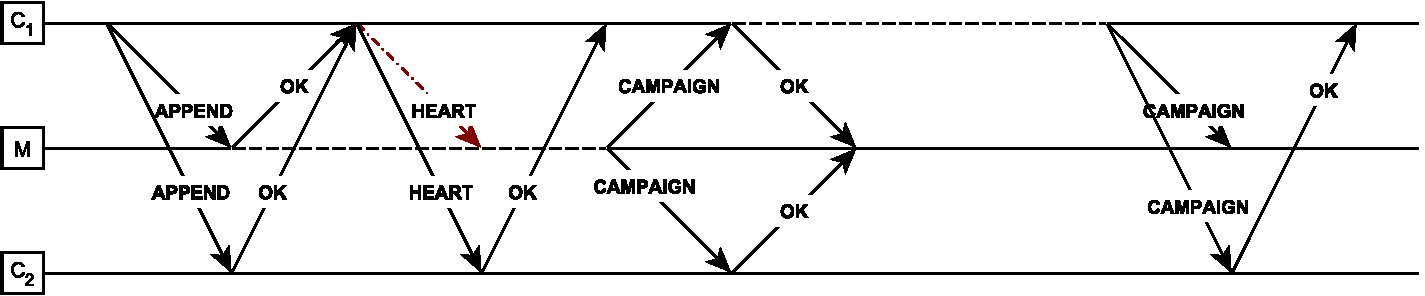
\includegraphics[width=\textwidth]{figures/raft-liveness-vuln.pdf}
	  \caption{Denial of service attack from malicious processor $M$ against correct processors $C_1$ and $C_2$. $M$ can repeat the above to continue the attack.}
	\end{figure}

	As previously discussed, Raft in its basic structure is vulnerable to disruption of liveness even after a byzantine transformation via SGX.
	A malicious processor may exploit this weakness by
	\begin{enumerate*}[label=\textbf{(\alph*)}]
	  \item dropping all heartbeat (empty append) messages from leaders when follower and
	  \item dropping all messages to and from any processor when leader.
	\end{enumerate*}
	As a result of \textbf{(a)}, the malicious processor will timeout and start an election whenever the leader has nothing to append for time period $\Delta_{min}$ (resulting in a heartbeat instead of regular append).
	The malicious processor is likely to win this election as, as the leader has not actually crashed.
	The correct processors will only contest such an election if the leader actually crashes or the network is sufficiently delayed.
	The malicious processor must not drop non-empty append messages, as a candidate must be up to date from the viewpoint of a majority of processors.

	As a result of \textbf{(b)}, immediately after becoming leader, the malicious processor will stop communicating with the rest of the network, causing correct processors to timeout and start yet another election.
	When a new leader is elected, the process starts over from \textbf{(a)}.
	In this situation, there is a window between \textbf{(b)} and \textbf{(a)} where a correct leader can append entries before the malicious processor becomes leader again.
	Thus, liveness may not be completely lost, but the throughput of the algorithm is negatively affected.
	If two malicious processors collude to swap leadership using the above strategy, liveness will be lost until the network becomes asynchronous and possibly elects a correct processor as leader.

	To mitigate the effect of this vulnerability, an extra message phase before a processor starts an election can be added~\cite{ongaro_search_2014}.
	In this pre-election phase, a timed out processor will poll the other processors on whether or not they would grant their vote in a potential election.
	The other processors will say yes if
	\begin{enumerate*}[label=\textbf{(\alph*)}]
	  \item the conditions of a normal election are fulfilled (newest term, have not voted in term, up-to-date log) and
	  \item they have not themselves received a message from the leader for time period $\Delta_{min}$.
	\end{enumerate*}
	Only after receiving a majority of pre-election endorsement, the timed out processor will increment its term and start a proper election.
	Because of \textbf{(b)} a malicious processor cannot convince an SGX-transformed Raft algorithm to start an election by dropping leader messages.

	\subsubsection*{Leader liveness vulnerability}
	\label{subsub:leader-liveness-vulnerability}

	Another liveness vulnerability exists when a malicious processor drops selected messages.
	A malicious processor can temporarily prevent liveness by
	\begin{enumerate*}[label=\textbf{(\alph*)}]
	  \item acting correctly while not elected as leader and
	  \item dropping all client messages when elected as leader.
	\end{enumerate*}
	The malicious processor will eventually become leader in an asynchronous setting following \textbf{(a)} and then prevent any commands to be committed following \textbf{(b)}.
	The most intuitive solution is allowing the client to accuse the leader of being malicious, forcing the remaining processors to elect a new leader.
	However, this solution opens the network up to a denial of service attack by a malicious client.
	A second solution allows a client to broadcast a command to all processors when unable to contact the leader.
	The processors will piggyback the broadcast command on their next message to the leader, forcing the leader to either drop all messages or appending the command.
	We have chosen to implement neither of these solutions and instead disregard the problem as it cannot permanently prevent liveness.
	Given the argument that \textbf{(a)} causes the malicious processor to eventually become leader, it follows that another processor will eventually overthrow the malicious processor, restoring liveness.

	\subsection{Protocol}
	\label{subsec:protocol}

	We use Raft to implement event locking (Section~\ref{subsec:execution-ordering}) and cluster consensus (Section~\ref{subsec:cluster-consensus}), by exploiting the guarantees given in Figure~\ref{fig:raft-properties}.
	We define three command types for accomplishing this:
	\begin{description}
	  \item[\normalfont$\MSG{\REQ\COMMAND, tag, e, \ENUM{LOCK}}$:] request the exclusive lock to execute event $e$.
	  \item[\normalfont$\MSG{\REQ\COMMAND, tag, e, \ENUM{ABORT}}$:] release the lock to execute event $e$ without modifying any state.
	  \item[\normalfont$\MSG{\REQ\COMMAND, tag, e, \ENUM{EXEC}}$:] execute the event $e$ and modify state accordingly.
	\end{description}
	Recall the definition of a DCR graph $G(E, R)$ comprising of event set $E$ and relation set $R$.
	Also recall the definition of the set of events to be locked when executing an event $e$ as $L(e)$ (semantically defined in Section~\ref{subsec:execution-ordering}).
	We define the set of processors replicating event $e$ (cluster for $e$) as $C(e)$ and their leader as $C_{leader}(e)$.
	With this we define the set of cluster leader processors that must be locked when executing en event $e$ as $L_{leaders}(e) = \bigcup_{e' \in L(e)} C_{leader}(e')$.
	We say $committed(entry, leader)$ is true iff $entry$ has been added to the log of $leader$ at index $i$ and $commit_i \ge i$.

	For processors in the leader state, we extend Raft with a state machine that can intercept incoming Raft messages, send new \ENUM{COMMAND} messages, and gets notified when a log entry is committed.

	\subsubsection*{Normal Operation}

	A cluster leader $p_l$ receives $\MSG{\REQ\COMMAND, tag_{lock}, e, \ENUM{LOCK}}$ requests from clients or other cluster leaders.
	During intercept the extension checks whether the leader's log is in a lockable state, which it does by checking if the last log entry is not a $\ENUM{LOCK}$ and, based on the log, is $e$ enabled.
	If no, respond with $\MSG{\RSP\COMMAND, tag_{lock}, false}$.
	If yes, pass the $\REQ\COMMAND$ request onto Raft.

	When a $(tag_{lock}, e, \ENUM{LOCK})$ entry is committed, a cluster leader will do one of two things:
	If $p_l \ne C_{leader}(e)$, $p_l$ is not responsible for the terminating the execution attempt.
	In this case we rely on Raft to respond to the $\REQ\COMMAND$ request to let $C_{leader}(e)$ know $p_l$'s cluster is locked for execution of $e$.
	If instead $p_l = C_{leader}(e)$, $p_l$ must continue terminating the execution attempt by locking $L(e)$.
	To do this $p_l$ sends $\MSG{\REQ\COMMAND, tag_{lock}, e, \ENUM{LOCK}}$ to processors $L_{leaders}(e)$.
	Notice the tag is reused for this secondary lock.
	Further, $p_l$ notes $lock_{count}(tag_{lock}) \leftarrow 0$.

	A cluster leader $p_l$ will intercept $\MSG{\RSP\COMMAND, tag, success}$ responses when the last log entry is $(tag_{lock}, e, \ENUM{LOCK})$ and $tag = tag_{lock}$.
	If $success = true$, $p_l$ increments $lock_{count}(tag_{lock})$.
	Otherwise a lock on the cluster of an event in $L(e)$ was denied and $p_l$ must abort the execution attempt.
	To do this $p_l$ simultaneously passes $\MSG{\REQ\COMMAND, tag_{abort}, e, \ENUM{ABORT}}$ to its Raft component and sends the request to $L_{leaders}(e)$.

	When $lock_{count}(tag_{lock}) = |L(e)|$, $e$ can safely be executed. $p_l$ sends $\MSG{\REQ\COMMAND, tag_{exec}, e, \ENUM{EXEC}}$, $m_{exec}$, to its Raft module.
	When $(tag_{exec}, e, \ENUM{EXEC})$ is committed, $p_l$ sends $m_{exec}$ to $L_{leaders}(e)$.

	\subsubsection*{Leader Recovery}

	As cluster leaders may crash at arbitrary times, we must be able to safely continue from any step of an execution attempt as a newly elected leader.
	We accomplish this mainly by exploiting the Leader Completeness property (Figure~\ref{fig:raft-properties}).
	After being elected, a new leader $p_l'$ will look at the most recent log entry to determine if it needs to restart a step to finish an execution attempt of a previous leader.
	Recall that an entry, which has been committed by a leader, will not necessarily be in the committed state for the successor.
	The Leader Completeness property only ensures that it will eventually be committed at the successor.
	If the last entry is not committed at $p_l'$, no action is needed as normal operation will handle when it eventually commits.
	Similarly, if the last entry is $(tag, e, type)$ where $p_l' \ne C_{leader}(e)$, no extra action is needed from $p_l'$.
	Otherwise if $p_l' = C_{leader}(e)$, branch on the last entry as follows:
	\begin{itemize}
	  \item $(tag_{lock}, e, \ENUM{LOCK})$\\
	  Send $\MSG{\REQ\COMMAND, tag_{lock}, e, \ENUM{LOCK}}$ to $L_{leaders}(e)$. Recall that $\REQ\COMMAND$ requests with the same tag will not result in duplicate entries. If the old leader already sent some or all of these requests, $p_l'$ will simply be notified of their result.
	  \item $(tag_{abort}, e, \ENUM{ABORT})$\\
	  Send $\MSG{\REQ\COMMAND, tag_{abort}, e, \ENUM{ABORT}}$ to $L_{leaders}(e)$.
	  \item $(tag_{exec}, e, \ENUM{EXEC})$\\
	  Send $\MSG{\REQ\COMMAND, tag_{exec}, e, \ENUM{EXEC}}$ to $L_{leaders}(e)$.
	\end{itemize}
	As a final note on leader recovery, we must ensure progress at some $p_l$ when attempting to execute $e$ even though leaders of $L_{leaders}(e)$ crash.
	This requires $p_l$ to resend any $\REQ\COMMAND$ requests which it does not receive corresponding $\RSP\COMMAND$ response for indefinitely.

	\subsubsection*{Termination Argument}

	\begin{figure}[t]
  	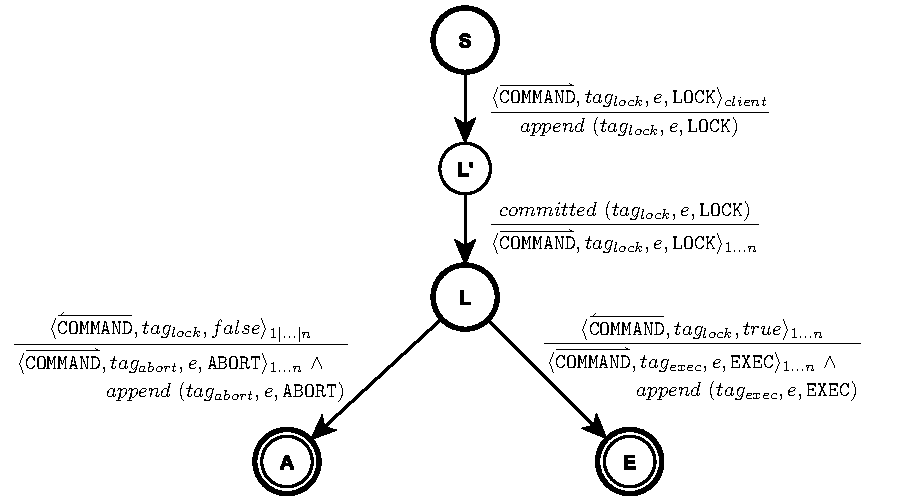
\includegraphics[width=\textwidth]{figures/raft-2pc.pdf}
	  \caption{State machine for $C_{leader}(e)$ during execution of $e$ with states start ($\bm{S}$), intermediate locked ($\bm{L}'$), locked ($\bm{L}$), abort ($\bm{A}$), and execute ($\bm{E}$). Similar to~\cite{skeen_nonblocking_1981} we show received and sent messages above and below the line subscripted with the origin or destination process. 
	  We also show appending and committing entries in $C(e)$ as messages.}
	  \label{fig:raft-2pc}
	\end{figure}

	This locking scheme is very similar to centralized two phase commit~\cite{skeen_nonblocking_1981}, where a leader safely advances a set of replicas to a commit or abort state.
	As described in~\cite{skeen_nonblocking_1981}, two phase commit is a blocking protocol, meaning a leader or replica processor crash will halt the system until the crashed processor recovers.
	This is still true for our application of the two phase commit protocol, but we have augmented each site with an event cluster.
	Because of this, a single processor crash cannot block the two phase commit.
	Blocking of an attempt to execute $e$ can occur at the earliest when a cluster in $\bigcup_{e' \in L(e)} C(e')$ experiences crashing of a majority of processors.

	To show our proposed algorithm always terminates, when no involved cluster experiences a majority crash, we will examine the event of a cluster leader crashing during an execution attempt.
	Specifically we will examine the $C(e)$ cluster when attempting to execute some event $e$, as the argument for termination at clusters $\bigcup_{e' \in L(e)} C(e')$ will follow naturally.
	After having entered state $\bm{L}'$ of Figure~\ref{fig:raft-2pc}, $C_{leader}(e)$ will have begun committing a lock entry at its cluster. 
	Because Leader Completeness only applies to committed entries, we need this extra state to ensure that a successor of $C_{leader}(e)$ will be aware of the lock.
	Was $C_{leader}(e)$ to append the lock entry locally while simultaneously commanding clusters $\bigcup_{e' \in L(e)} C(e')$ to append the lock entry, we risk that a successor of $C_{leader}(e)$ would be unaware of the lock commands by its predecessor resulting in a stuck state for $\bigcup_{e' \in L(e)} C(e')$.
	If $C_{leader}(e)$ crashes at $\bm{L}'$, the lock entry will either exist in the successor's log meaning that we simply continue, or it will be lost meaning that the successor goes to state $\bm{S}$.
	This is fine as the client requesting the execution must be ready to resend commands, when leaders crash, as per the Raft algorithm design.

	At state $L$ a crash of $C_{leader}(e)$ is safe, as Leader Completeness guarantees the lock to be known by the successor.
	By redoing the $\bm{L}' \rightarrow \bm{L}$ transition, the successor can safely re-enter $\bm{L}$ as duplicate command messages are allowed by Raft.

	Notice when transitioning from $\bm{L}$ to $\bm{A}$ or $\bm{E}$, no intermediate state is needed and an entry can be appended to $C(e)$ simultaneously with sending commands to $\bigcup_{e' \in L(e)} C(e')$.
	If $C_{leader}$ crashes at $\bm{A}$ or $\bm{E}$, a successor risks moving back to $\bm{L}'$, as the $\ENUM{ABORT}$ or $\ENUM{EXEC}$ entry may be lost completely and the $\ENUM{LOCK}$ entry may not yet be committed at the successor.
	It is possible to prevent this by introducing intermediate states $\bm{A}'$ and $\bm{E}'$, but it is not necessary to guarantee termination.
	Commands can be re-sent without resulting in duplicate entries as long as the tag remains the same.
	Thus, if a successor of a leader in state $\bm{A}$ or $\bm{E}$ is in state $\bm{L}'$, it will simply redo the commands for $\bm{L'} \rightarrow \bm{L}$ followed by $\bm{L} \rightarrow \bm{A}$ or $\bm{L} \rightarrow \bm{E}$.
	This is guaranteed to result in the same state as the predecessor, as two different command responses for the same tag are impossible by the properties of Raft~\ref{fig:raft-properties}.

	\subsubsection*{Complexity}

	The resulting protocol has the following properties when achieving consensus on an execution with regards to message complexity
	When an execution is initiated in a cluster, that cluster must first achieve consensus on the decision to initiate an execution.
	Then locking is performed in the cluster and when it has been committed, locking is attempted on the cluster of each other event to be locked.
	Once all locks have been obtained, the locked processes are notified of the execution on which they must now achieve consensus.
	This results in a message complexity of $O(m\cdot \|E_{aff}(G, e) \cup L(e)\|)$, where $m$ is the size of a cluster\footnote{This is assuming that each cluster has the same size. Otherwise the average cluster size should suffice.} and $G$ is the graph on which the event, $e$, is executed.
	If any leader crashes or a faulty channel causes all messages to be lost, this complexity no longer holds, as leader crashes would require leader recovery which has a message complexity of $O(n)$ which can happen up to the fault tolerance of $f$ for each cluster.
	Note that if a channel loses all messages put through it, indefinitely, the relaxed liveness guarantee of Raft means that termination would no longer be guaranteed in this case.

	\section{Security analysis}
    \label{sec:security-analysis}

	The following is a security analysis of the algorithm described in Section~\ref{sec:analysis}.

		\subsection{Adversary model}

		We allow for a strong adversary model known as the Dolev-Yao adversary~\cite{dolev_security_1983}.
		The Dolev-Yao adversary can intercept, tamper with, delay and duplicate all messages in the system, as well as create new messages.
		However, the Dolev-Yao adversary cannot guess the cryptographic secrets in the system.

		In a system with no cryptographic security, such an adversary can, by utilizing these techniques completely impersonate any and all processes by intercepting all messages for a process, and creating new messages seemingly originating from that process.
		From the perspective of a correct process in such a system, a Dolev-Yao adversary can make any other process exhibit arbitrary behaviour and even coordinate the behaviour of all other processes by utilizing this impersonation attack.
		Notice that such an attack would present as byzantine faults for any correct process, as that process would interpret all impersonated messages as correct, and thus experience other processes as behaving arbitrarily.
		In a system with cryptographically signed or MAC'ed messages, however, the Dolev-Yao adversary cannot impersonate any such message, since they cannot guess the cryptographic secrets.
		Notice that it is a quite strong assumption that the adversary cannot guess this system's cryptographic secrets, in that Intel could theoretically be an adversary and would in that case know the processor specific PID key, which is essential for the Remote Attestation secret provisioning in the SGX transformation in Section~\ref{sec:transforming-byzantine-faults}.

		\subsection{Analysis}

        We will now show that the worst attack an adversary can mount on our system is a liveness attack, under our system model an adversary assumptions.
        This will be followed by examples of liveness vulnerabilities, including an argument for the impossibility of protecting against these attacks.

		Since the SGX transformation in Section~\ref{sec:transforming-byzantine-faults} results in all messages being MACed by a common secret key, any messages created by the adversary will dropped by all integrity protected subprocesses, due to the messages having incorrect MACs.
        Thereby the adversary only have the possibility of creating messages that are accepted by the wrapper-components, but not the underlying integrity protected components.
        But as the wrapper-components only serve to pass messages, this is the same as tampering with the channels as shown in Section~\ref{sec:transforming-byzantine-faults}.
        Similarly, tampering with any message originating from an integrity protected subprocess, will be discarded when received by any other integrity protected subprocess.
        As such, an adversary can at most mount attacks using by message omissions, duplications and  delays.
        Using these abilities, the adversary can simulate crashes by omitting all messages to and from a process.
        With these restraints, an adversary can induce several attacks on liveness:

		With message omissions and message delays, the adversary is able to give any correct process a cluster leadership.
		They can do this by omitting all messages from the current leader, and omitting all messages from candidates timing out before candidate process desired to be leader by the adversary.
        This is in and of itself not problematic, since the adversary can only cause correct processes to become leader, as faulty processes does not produce correctly MACed messages.
        However, from this technique arises two liveness attacks.

		By chaining these leader election attacks without resolving any of them, they can mount an attack on the liveness of a cluster.
		One such chain could looks like this: omit messages from the leader to $f+1$ processes until one of them, $p_1$, becomes a candidate.
		Then omit messages from $p_1$ to $f+1$ other processes, until another process, $p_2$, becomes a candidate and repeat forever.
		Thereby the cluster will stay in a continuous election process, and cannot commit any client requests.
        Under more weak adversary assumptions, where the adversary cannot continue omitting messages indefinitely, the cluster will eventually successfully complete an election, and resume correct operation, however.
		And due to the pre-election phase, the original leader will still be the leader after the attack has been terminated.
		As such, any valid requests received by the leader will eventually be agreed upon after the attack has been terminated, if the leader does not crash during or immediately after the attack.

		In the proof of FLP-impossibility~\cite{fischer_impossibility_1985}, the authors shows that there will always exist a sequence of message omissions that violates availability (i.e. liveness in SMR), if the system is an asynchronous setting and handles crashing processes.
		Therefore, we can conclude that any fault-tolerant SMR in an asynchronous setting will be vulnerable to such an attack under a Dolev-Yao adversary.
		The sequence of message omissions that violates liveness in Raft is present under the leader election; any unresolved heartbeat will eventually result in a leader election, which might then never terminate if no process wins the election, which is what the adversary exploits in this attack.

		Another attack on liveness is described in Section~\ref{subsub:leader-liveness-vulnerability}.
		The attack consists of the adversary omitting all client messages to the leader of cluster.
		By doing this, the adversary does not only attack the liveness of that cluster, but also all other clusters for which an execution requires a lock on the cluster under attack.
		We argue in Section~\ref{subsub:leader-liveness-vulnerability} that eventually a new process will become the leader, which prevents an indefinite liveness attack.
		However, under a Dolev-Yao adversary, the adversary can prevent any other process in winning the election, thus prolonging the liveness attack indefinitely.
		A solution is also described in Section~\ref{subsub:leader-liveness-vulnerability}, in which clients that does not receive a response in due time will broadcast to the entire cluster, which will force the leader to either accept the request, or force a leader change in the cluster.
		However, this solution does not necessarily prevent the attack, since the adversary intercept the client broadcast.

		Notice that both these attacks targets a single cluster, and therefore at most affect a subset of the clusters that make up the entire system.
		We have not identified any single attacks that spans the entire system.
		If the adversary wants to mount an attack on the entire system that prevents liveness in any state of the graph, they must mount a liveness attack on a subset of clusters $A$ for which $\forall e \in A.\ \nexists e'.\ e' \in I_{stat}(e) \land e' \not \in A$.
		In other words, the subset of clusters must contain all events that are statically independent.
		Calculating $I_{stat}(e)$ of a all $e's$ is infeasible for large enough graphs (see Section~\ref{subsubsec:concurrency}), so the adversary must either attack an approximation, or all clusters, both of which are inefficient solutions.
		An alternative is to attack the clusters of all dynamically independent event for the current $G$ state, but the adversary is not guaranteed that the global history reported by the log-augmented snapshot described in~\ref{subsec:global-history-collection} is current, and is therefore not guaranteed that their attack will completely prevent any further execution of graph.
		So an adversary must mount a suboptimal attack to prevent liveness in the entire system.

		Safety cannot be attacked under the limitations of our adversary.
        This is due to the fact that our adversary can only utilize message omissions, duplications and process crashes in our system, under all of which Raft guarantees safety~\cite{ongaro_search_2014}.

        Summarized, the system is vulnerable to liveness attacks.
        This due to the underlying SMR protocol (Raft), which solves the consensus problem in an asynchronous system with crashes, and thus must have a sequence of message omissions that violate liveness.
        However, by the guarantees of the Raft algorithm, the system is not vulnerable to any safety attacks.

	\section{Secure DCR Implementation}

	\begin{figure}[t]
		\centering
		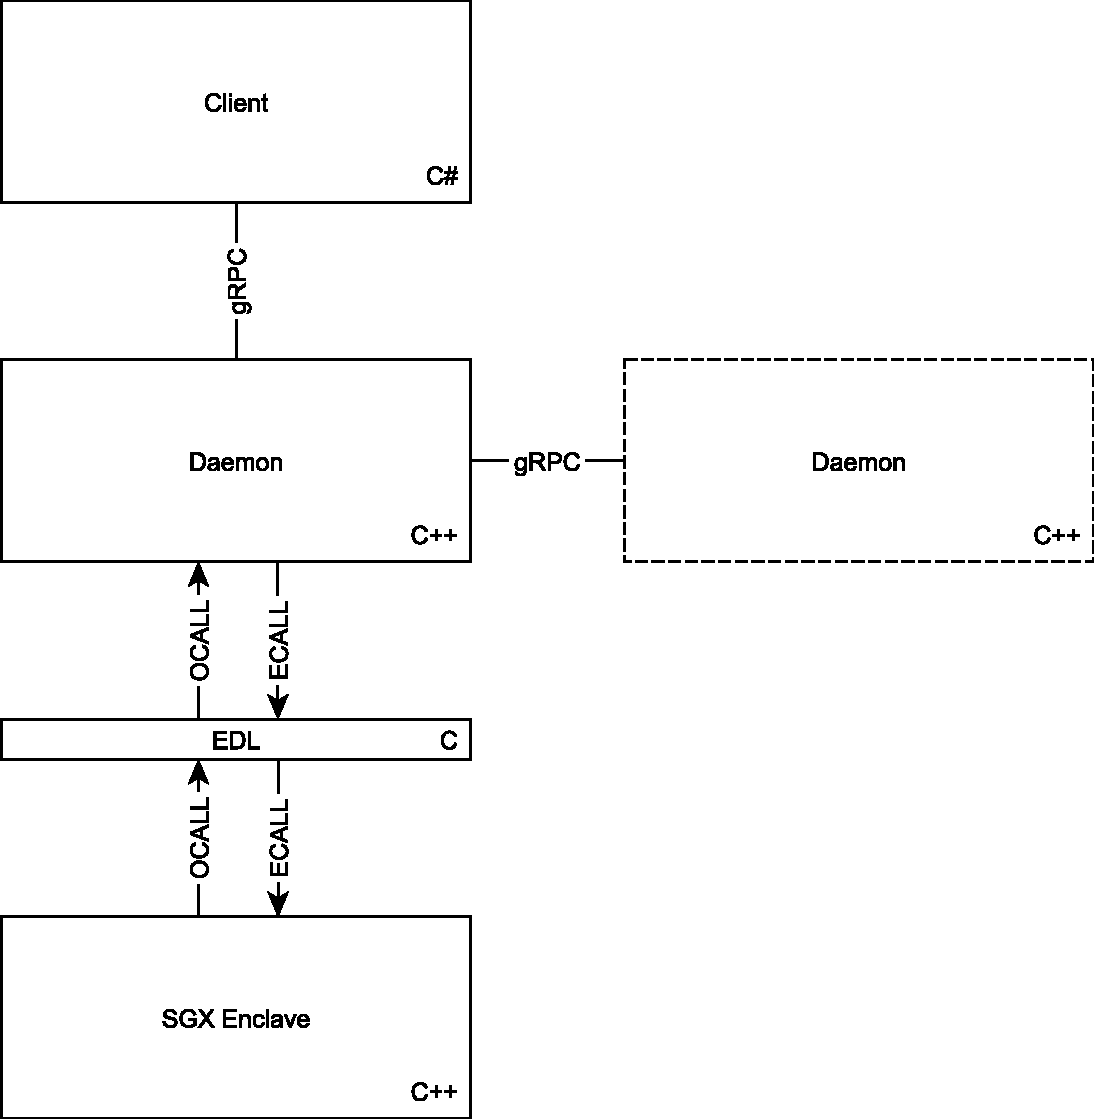
\includegraphics[width=\textwidth]{figures/dcr-graphs/network-stack.pdf}
		\caption{Figure showing the components of the trusted DCR implementation.
		The rectangles are the components themselves and the lines are the channels which are used for communication between the connected components. }
		\label{fig:network-stack}
	\end{figure}

	As a proof-of-concept, we have implemented the system discussed in Section~\ref{subsec:protocol}.
	The system consists of an implementation of the Raft~\cite{ongaro_search_2014} algorithm augmented with our protocol for DCR execution.
	Further, this implementation is hardened against Byzantine faults via the transformation described in Section~\ref{sec:transforming-byzantine-faults}.
	The implementation in its entirety can be found at \url{https://github.com/trusted-dcr}.

	Figure~\ref{fig:network-stack} shows an overview of the system.
	An SGX enclave drives the major parts of the system.
	Both Raft and a DCR execution engine exists inside the protected enclave environment, preventing Byzantine faults at these components.
	However, the enclave does not have access to the network stack of the system it is running on.
	To provide inter-peer communication, the enclave instead contacts a daemon using O/ECALLs.
	This call interface is defined in the Enclave Definition Language (EDL)~\cite{intel_sgx_guide} layer.

	\subsection{SGX Enclave}

	The enclave protects the classical Raft algorithm against Byzantine faults as described in Section~\ref{sec:transforming-byzantine-faults}.
	All Raft messages are augmented with a message authentication code (MAC) using a key shared between all peers.
	The shared key is obtained through attestation and is confidential to the enclaves (meaning that it can never leave protected memory).\footnote{The implementation does not currently use SGX attestation for key distribution, but instead relies on an unsafe hard-coded shared key.}

	\subsection{EDL}

	Using our EDL definitions, the SGX SDK generates a secure call interface between the trusted enclave and the untrusted daemon.
	Specifically, the call interface
	\begin{enumerate*}[label=\textbf{(\alph*)}]
		\item limits all external interaction with the enclave to exactly what is defined by the EDL definitions,
		\item prevents leaking protected memory through pointers by first copying structures to a zeroed scratch space, and
		\item prevents concurrent calls to the enclave unless explicitly allowed.
	\end{enumerate*}

	An excerpt of the enclave--daemon interface definition can be seen in Listing~\ref{listing:edl}.
	The trusted part defines ECALLs, allowing untrusted code to call enclave functions.
	The untrusted part defines OCALLs, allowing the enclave to call untrusted functions outside the enclave.
	Listing~\ref{listing:edl} shows trusted functions for the enclave to receive network messages from the daemon and untrusted functions for the enclave to send network messages to the daemon.

	The considerations of \textbf{(b)} are apparent in the untrusted \texttt{send\_append\_req} function.
	Here the structure \texttt{append\_req\_t} contains a pointer to a range of entries.
	Inside of the enclave, such a pointer would map to protected memory, which is inaccessible to the untrusted function definition.
	Therefore the pointer is extracted from the structure and given as a parameter tagged with \texttt{[in, count=size]}.
	The \texttt{in}-part causes the interface to create a scratch space in unprotected memory, where the entries are copied to, allowing the untrusted function access~\cite{intel_sgx_developer_reference}.

	While the enclave can be written in \cpp, EDL is a superset of plain C.
	This means a lot of work goes into converting from \cpp types, like vectors and maps, to types consumable by the EDL layer.

	\begin{snippet}
		\begin{mdframed}[backgroundcolor=Papyrus]
			\begin{lstlisting}[basicstyle=\small\ttfamily]
enclave {
  ...
  trusted {
    ...
    public void recv_append_req(append_req_t req);
    public void recv_append_rsp(append_rsp_t rsp);
    ...
  };

  untrusted {
    ...
    void send_append_req(
    	append_req_t req,
    	[in, count=size] entry_t* entries,
    	int size);
    void send_append_rsp(append_rsp_t rsp);
    ...
  };
};
			\end{lstlisting}
		\end{mdframed}
		\caption{Excerpt from the \texttt{enclave.edl} file.}
		\label{listing:edl}
	\end{snippet}

	\subsection{Daemon}

	As the enclave cannot communicate directly with the network stack of the system, a daemon is needed for inter-peer communication.
	The daemon implements OCALLs for sending messages, parametrised by the ID of the target peer.
	The enclave uses these OCALLs for all message passing.
	Messages heading in the opposite directed are passed to the enclave via an ECALL by the daemon.

	Inter-peer communication uses TCP for all messages.
	Specifically, the daemon implements a gRPC server and client.
	Note that there is no particular reason to use gRPC or even TCP other than for ease of implementation.

	The daemon also facilitates user input into the enclave, as the enclave has no access to the command line.
	During start up, the daemon sends a configuration message to the enclave.
	This configuration is primarily constructed at the client and passed to the daemon, again via gRPC.
	It contains the DCR graph, cluster memberships, and the ID of the local enclave.
	In the current implementation, the configuration also includes a hard-coded mapping between peer IDs and IP addresses.
	During attestation, peers must agree on this configuration.
	Otherwise a malicious actor would be able operate in the network with a less restrictive configuration\footnote{The configuration should map client public keys with events if authentication is needed for execution. This functionality does not currently exist in the implementation.}.

	\subsection{Client}

	Finally a simple command line interface has been implemented as a client.
	This client is capable of communicating with the daemon to configure the enclave, initialise it, perform executions and fetch the global execution history.
	Configuration is handled using a JSON configuration file.
	After parsing the configuration, the client starts the daemon process and transmits the configuration via gRPC.
	Execution and global history requests are similarly handled through gRPC calls to the daemon.
	After receiving an execution or history request, the daemon will use an ECALL to start the operation.
	When completed, the results are communicated back to the daemon and later the client via OCALLs and gRPC\footnote{In the current implementation, the client is not notified when and if the execution succeeds.}.
	When fetching the global execution history, the client will create a consistent cut from the logs retrieved by the daemon and validated by the local enclave, as described in Section~\ref{subsec:global-history-collection}.

	\section{Distributed Smart Contract Engine}

	The system described in this thesis, which solves the problem of a partial state DCR engine in a byzantine setting, can be converted to support a variety of programs, much like Ethereum.
	The classic Ethereum example is the Decentralized Autonomous Organization (DAO), which is was a decentralized investment fund, where an Ethereum peer could invest some money and be paid in kind if the investment made by the DAO earned money.
	What the DAO actually invested in was decided by the peers who voted, weighted by how much money they had placed into the DAO.

	If a system like the DAO were to be implemented into a general version of the DCR engine described in this thesis, a transformation of the state is required.
	We start this transformation by redefining events to contain an arbitrary amount of data, rather than the DCR state of its executed, included and pending attributes.
	Since the state of an event can now be arbitrary, a more generalised version of effects and constraints are required.
	\begin{description}
		\item[Effects] applies the specified modification to the state of target event.
		\item[Constraints] specifies whether or not the target event is executable, based on a set of criteria on the originating event.
	\end{description}

	\begin{figure}[t]
  	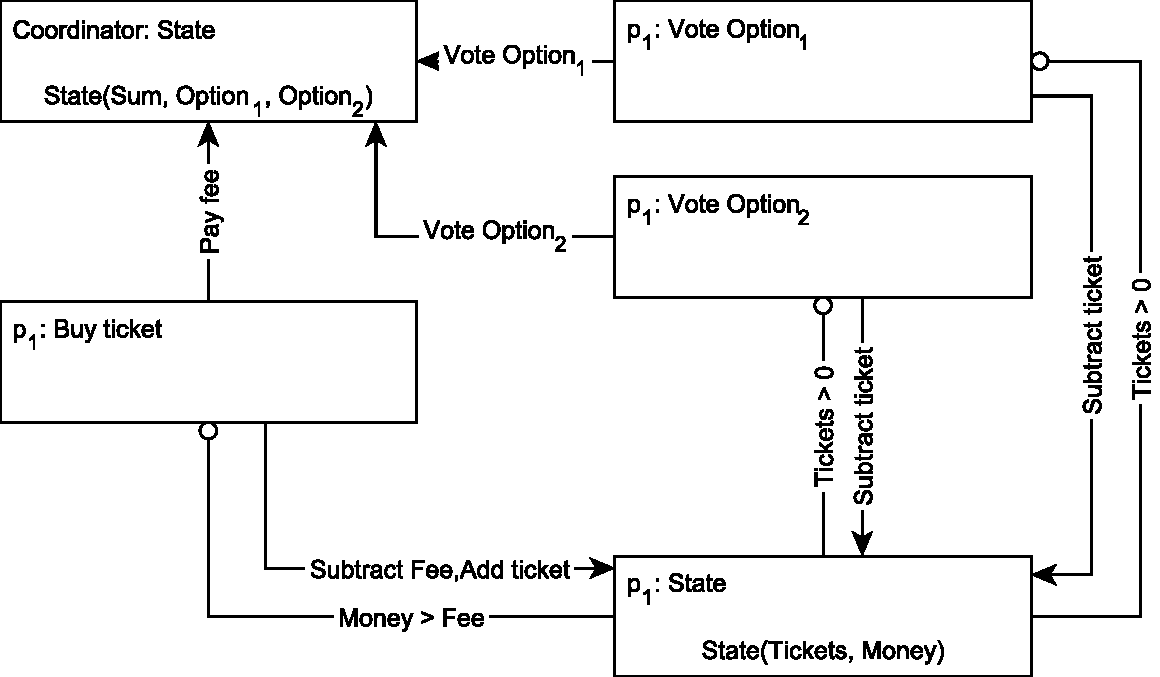
\includegraphics[width=\textwidth]{figures/dcr-graphs/dao-simple.pdf}
	  \caption{The simple implementation of the DAO.
	  The lines ending in arrowheads are effects and the lines ending in circles are conditions. }
	  \label{fig:dao-simple}
	\end{figure}

	We can now define implement the DAO in our transformed system, as shown in Figure~\ref{fig:dao-simple}.
	The figure shows five events, one of which is executable by the coordinator of the DAO and the rest of which are executable by a peer, $p_1$.
	We distribute the weight of votes by selling \textit{tickets} at a set price.
	The coordinator maintains a state consisting of the current sum of money placed in the DAO, the number of votes for investment option 1 and the number of votes for option 2.
	$p_1$ has can execute the following events:
	\begin{description}
		\item[State] which is the event containing the state of $p_1$. This event has no effect on execution.
		\item[Buy ticket] which on execution subtracts the fee of a ticket from the state of $p_1$, adds a ticket to the state of $p_1$ and adds the fee to the state of the coordinator.
		Note that this event can only be executed if $p_1$ has enough money.
		\item[Vote option$_\textbf{1}$] which on execution adds a ticket to the vote tally of option$_1$ kept by the coordinator and removes a ticket from the state of $p_1$.
		This event can only be executed when $p_1$ has a ticket to spend.
		\item[Vote option$_\textbf{2}$] which on execution adds a ticket to the vote tally of option$_2$ kept by the coordinator and removes a ticket from the state of $p_1$.
		This event can only be executed when $p_1$ has a ticket to spend.
	\end{description}
	Note that the state of $p_1$ could be stored in each event belonging to $p_1$, but as this would require the events of $p_1$ to subtract tickets and money from all occurrences of the state of $p_1$, the state is kept separately in order to reduce the complexity of the example.
	This subsystem of events belonging to $p_1$ can be duplicated for each respective peer which participates in the DAO.
	Note that performing the investment itself is illustrated in the example, but could easily be accomplished by having events deciding for option$_1$ and option$_2$.
	Option$_1$ would only be executable if every peer has spent their tickets and option$_1$ has more votes than option$_2$.
	The inverse would be true for Option$_2$.
	Additional state would be needed in order to return the correct amount of money back to the investors, but that should be trivial given the functionality displayed in this example.

	Due to the way the DCR engine is defined, all events and relations must be created simultaneously with the creation of the graph.
	This is limiting, in that events can only interact with each other in very specific predefined ways, such as the separate events for voting for option$_1$ and option$_2$ respectively.
	We could however improve the simplicity of the solution by introducing the concept of parametrised effects.

	\begin{figure}[t]
  	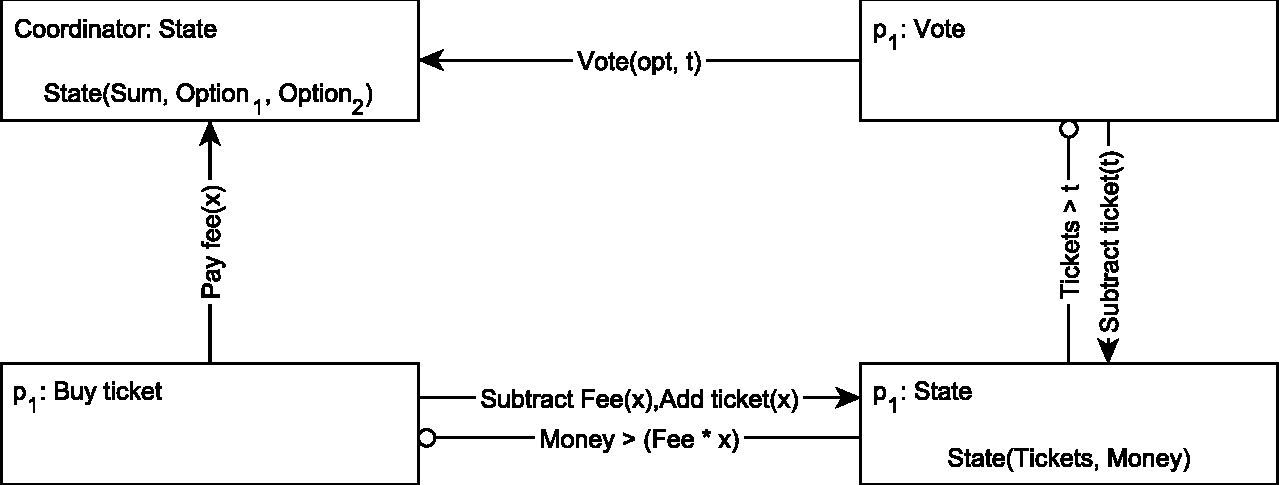
\includegraphics[width=\textwidth]{figures/dcr-graphs/dao-parametrised.pdf}
	  \caption{The parametrised implementation of the DAO.}
	  \label{fig:dao-parametrised}
	\end{figure}

	In Figure~\ref{fig:dao-parametrised} the DAO is shown implemented with parametrised effects.
	When an event is executed, it is supplied with the required variables.
	For example, when the \textit{Vote} event is executed, it is supplied with the option to be voted for, \textit{opt}, and how many tickets to assign in that vote, \textit{t}.
	An even more condensed parametrised version of this example could be created, by representing all of the events executable by $p_1$ as a single event and denoting what the execution of that event should do using parameters.

	The execution ordering semantics described in Section~\ref{subsec:execution-ordering}, largely still apply to this transformation, with the exception that an event does not have to lock itself when executing.
	This is because executing an event does not necessarily affect the event itself, unless an explicit effect is defined targeting it.

	\section{Discussion}

	We will now provide some perspective on the contributions of this thesis in relation to other solutions and the considerations of the solution presented here.

    \subsection{Security of SGX}

	All aforementioned security guarantees are derived by the confidentiality and integrity guarantees given by Intel, but since very little of the proprietary technology is documented, or documented contradictory in different documentations as noted in~\cite{costan_intel_2016}, all security assumptions of SGX rely on trust in Intel's implementation.
    While an argument can be made that every security critical protocol must to some extent trust the manufacturer of the hardware on which the protocol runs, Intel has historically had vulnerabilities in components similar to SGX.
    For example the CVE-2017-5689 security incident named \textit{Silent Bob} exposed in~\cite{silent_bob}, which allowed unprivileged access to the Intel Active Management Technology.

    Intel Active Management Technology is a component made for controlling networked host devices remotely, and is completely independent of the OS.
    The Silent Bob vulnerability allowed an adversary complete Admin\footnote{A role specific to the Intel Active Management Technology.} access to the Intel Active Management Technology, which roughly gave them the same possibilities as physical access to the host device.
    Such a vulnerability in SGX could potentially invalidate the security analysis presented in Section~\ref{sec:security-analysis}.
    We will therefore shortly present the most pertinent SGX vulnerabilities found at the time of writing, and assess the implications for the described system.

    As mentioned SGX does not protect against flawed software, so it is up to the developer to prevent side-channel attacks through OCALLs that might expose secret data.
	A noteworthy mention to illustrate the vigour needed is the common pitfall mentioned in~\cite{intel_sgx_guide} when using ECALLs and OCALLs.
	Because enclaves are compiled using a standard \cpp-compiler, structure padding is likely to happen.
	The SGX environment does not protect against leaking secret information through uninitialized structure padding when passing structures in ECALLs and OCALLs | this, and other common security pitfalls, are not part of any SGX security guarantees.
	Intel recommends to always clear secrets from the enclave memory after use in~\cite{intel_sgx_guide}, regardless of the guarantees given by the PRM, underlining the risk of unintended vulnerabilities.

    Recall that Intel claims that SGX provides confidentiality and integrity for running enclaves.
    To the best of our knowledge, no integrity vulnerabilities have been identified at the time of writing.
    However, a number of confidentiality vulnerabilities have been identified, most notably in~\cite{costan_intel_2016} and~\cite{chen_sgxpectre_2018}.
	\cite{costan_intel_2016} shows several issues regarding confidentiality, most notably an address translation attack, a cache timing attack and an instruction snooping attack.

    The address translation attacks utilises the fact that enclaves use the system page table even for data residing on PRM.
    As such it is possible for untrusted software to learn the page access order by manipulating the OS-controlled page table.
	Another possible attack vector is to perform cache timing by cleverly choosing the physical memory position of enclave memory pages on set associative caches.
	By mapping snooping software to the same cache set as the enclave, the snooping software can evict the enclave's memory from the cache and use timing to figure out if it is accessed again.
    \cite{costan_intel_2016} also identifies a vulnerability in utilising hyper-threading to snoop instructions run by the enclave process. A snooping process sharing physical core with an enclave can use performance counters to determine which instructions the out-of-order scheduler is able to run in parallel with the enclave.
	The presence of these attacks means that enclaves using data-dependent memory access will likely not ensure confidentiality.

	Lastly, it is shown in~\cite{chen_sgxpectre_2018} that SGX is vulnerable to a variant of the infamous \textit{Spectre} vulnerability.
	The Spectre vulnerability on SGX, so-called \textit{SgxPectre}, can be exploited by utilising out-of-order execution to influencing branch prediction and force an enclave process to load confidential data into the cache.
	The changes in the cache can then be read, so by flushing the cache with known data before-hand, an adversary knows exactly the data that has been loaded into the cache.

	Notice that all of these attacks requires physical access to the device running, and therefore does not at first glance seem overly dangerous for our system.
	However, our SGX transformation uses a symmetric key for the MAC'ing of our messages, as described in Section~\ref{sec:transforming-byzantine-faults}.
	As such the same secret is shared between all of the processes running in our system, and an adversary needs only access to any one of them, to gain access to the key.
	But since any process running the enclave on a SGX enabled device can be provisioned with the shared secret through remote attestation, this means that an adversary only needs access to any SGX enabled device and the correct enclave, to potentially gain access to the shared secret.
	This is of course a serious security concern, as access to the shared secret enables an adversary to introduce byzantine failures, by sending inconsistent messages while impersonating any process.
	And since the underlying Raft algorithm is not byzantine fault safe, the system would begin to exhibit undocumented behaviour.

	To solve this problem, we could introduce authentication in the remote attestation protocol, so that only participants in the workflow would be attested.
	However, this would not protect against a malicious participant, who could control the workflow by impersonating leader processes.

	Another solution is to remotely attest each message, i.e. requiring that each message is verified as being correct by a remote attestation service, which will then sign the message for the process.
	This solution is essentially a central server solution, and would introduce a single point of failure as well as the remote attestation server as a bottleneck of messages.

	In conclusion, we have not identified a simple solution to these vulnerabilities, and advise against using the system for security critical workflows until the aforementioned vulnerabilities have been addressed and secured by Intel.

	\subsection{Scalability and fault tolerance}

    One of the central aspects of our system, is the separation of state, i.e. each cluster stores a different state and keeps it updated.
   	This allows for high scalability, in that we can execute events in $O(m \cdot E_{eff}(G,e) + 1)$ messages, where $m$ is size of the clusters.
   	It will trivially be true that $n \geq m \cdot E_{eff}(G,e) + 1$, and for some graphs $n > m \cdot E_{eff}(G,e) + 1$, as described in Section~\ref{subsubsec:concurrency} and~\ref{sec:analysis}.

    An argument could be made that reducing $n$ in an SMR approach can achieve the exact same message complexity and fault tolerance, since the relationship between scalability and fault tolerance is highly interdependent in these approaches.
    To show this relationship, lets look at an example with $3$ statically independent events and $15$ peers in the network.
    In an SMR protocol, where all peers share the entirety of the state, and which achieves consensus in $O(n)$ messages under no faults, and has a fault tolerance of $f = \lfloor \frac{n-1}{2} \rfloor$, we can achieve an execution of an event in $k \cdot 15$ messages, where $k$ is some constant, with a fault tolerance of $7$.
    Our solution, where we distribute the state evenly in clusters (in this case $5$ peers per cluster), commits an execution in the system in $k \cdot 5$ messages with a fault tolerance of $2$.
    However, if we reduce the peer size in the SMR to $5$, we achieve exactly the same properties in terms required messages and fault tolerance, which begs the question of what properties we have actually achieved by the distribution of the workflow.

    The four major improvements over an SMR solution we have identified are:
    \begin{itemize}
    	\item Event executions are no longer bounded by a single leader's capacity.
	    In a high intensity workflow, with many concurrent event executions, an SMR solution would be bounded by the leader's network and computational capacity.
	    In our solution, the concurrent executions are performed on different leaders with no intercommunication, and thus we are instead bounded by the cumulated capacity all leaders.
    	\item A faulty cluster at most affect liveness of the clusters holding $D_{stat}(e)$, not the entire workflow.
	    If a cluster experiences $f+1$ crashes, liveness can no longer be guaranteed.
	    However, a cluster with no liveness does not necessarily completely halt execution of the workflow, as all clusters for the events in $I_{stat}(e)$ can never be affected by $e$.
    	\item A peer need only store part of the workflow, not the entire workflow.
    	Any peer in the cluster responsible for $e$ need only store the state of $e$ and the executions that effect $e$, which is bounded by $N(N(e)) \cup N(e) \cup e$, where $N$ denotes the neighbourhood.
    	\item In a comparison between our solution and an SMR solution with a fixed number of peers, the former achieves superior message complexity.
    	Lastly, in a setting where the number of peers are given, for instance due to hardware or legal restraints, we gain a better message complexity than SMR, at the expense of a lower fault tolerance.
    \end{itemize}

    \subsection{Comparisons}

	As there is only one other solution to the problem of byzantine fault tolerant distributed DCR our ability to compare our solution to others is limited.
	The existing implementation is on the Ethereum~\cite{_ethereum_2018} blockchain, which supports arbitrary smart contracts and on which a DCR engine has been created.
	In the Ethereum DCR project~\cite{madsen_collaboration_2018}, a DCR engine is implemented in the Ethereum specific language, Solidity, and created as a smart contract on the Ethereum blockchain.
	Smart contracts on the Ethereum blockchain, expose an API which any Ethereum user can call, provided that they compensate the network for processing that call.
	The guarantees provided by the blockchain are thereby extended to each and every smart contract on the platform, as all miners process the computations performed by all paying users.
	Aside from the blockchain constraint of a certain block frequency there is therefore also the added monetary costs associated with an execution.
	Since the DCR engine implemented in SGX has no monetary costs associated with it and the message complexity of performing an execution in the Ethereum DCR engine is not readily available or relevant, the block frequency is the only comparable quantity between the two.
	Ethereum has an average block frequency of 15 seconds at this time which means that performing a series of executions takes a considerable amount of time, compared to the trusted DCR engine.
	Additionally, the cost of creating a workflow and performing executions on it is by no means trivial (6.6 USD in the example graph, at the time of that article's writing).
	There is, however, significant advantages associated with the Ethereum solution, in that the fault tolerance is not based on the users of the DCR engine, but rather the users of Ethereum, which is currently of considerable size.
	The sheer size of the Ethereum network therefore makes it incredibly resilient to attacks and practically guarantees availability, as each Ethereum node holds the state of the network.
	A main concern with the trusted DCR project was scalability and as joining the Ethereum network entails storing the state of all smart contracts, the DCR engine running on Ethereum should only be used in cases where scalability is of absolutely no concern.

	\section{Conclusion}

	In this thesis we have explored the usages of Intel SGX with regards to the problem of partial state machine replication with DCR graphs serving as the state.
	We have described a transformation of any distributed crash-fault tolerant algorithm to a byzantine fault tolerant algorithm using SGX and are the first to do so, as far as we are aware.
	Using this transformation, we have developed a consensus algorithm which forms part of a highly concurrent and scalable solution to the problem of decentralised, state-distributed DCR graphs.
	Lastly we have also demonstrated that the designed partial state algorithm is not limited to running DCR graphs.

	Specifically with regards to DCR, this thesis presents the first byzantine fault tolerant state-distributed DCR engine accompanied by an in-depth analysis of the necessity for execution ordering in DCR.
	Beyond that, the presented solution to the PSMR problem goes beyond any existing solution in terms of the combination of a low number of messages required for updating the state, $O(m)$ and the high fault tolerance of $f = \lfloor\frac{n-1}{2}\rfloor$.

	\newpage
	\bibliography{bibliography}{}
	\bibliographystyle{plain}

	\newpage

	\appendix
	\section{Raft Pseudocode}
	\begin{mdframed}[backgroundcolor=Papyrus]
	\begin{lstlisting}[style=pseudo, caption={All message types.}]
$\MSG{\REQ\COMMAND, tag, event, type}$
$\MSG{\RSP\COMMAND, tag, success, leader}$

$\MSG{\REQ\APPEND, term, prev_t, prev_i, commit_i, entries}$
$\MSG{\RSP\APPEND, term, prev_t, prev_i, success, last_i}$

$\MSG{\REQ\POLL, term, last_t, last_i}$
$\MSG{\RSP\POLL, term, success}$

$\MSG{\REQ\ELECTION, term, last_t, last_i}$
$\MSG{\RSP\ELECTION, term, success}$
	\end{lstlisting}
	\end{mdframed}

	\begin{mdframed}[backgroundcolor=Papyrus]
	\begin{lstlisting}[style=pseudo, caption={Logic shared between follower, candidate and leader states.}]
$log \leftarrow []$
$term \leftarrow 0$
$commit_i \leftarrow 0$
$indices[p_1 \dots p_n] \leftarrow 0$

$\tau_{min} \leftarrow nil$
$\tau \leftarrow nil$

$endorsement \leftarrow nil$
$votes_{poll} \leftarrow 1$
$votes_{election} \leftarrow 1$
$p_l \leftarrow nil$

function last_entry()
  return $log[|log| - 1]$

function update_timeout()
  $\tau_{min} \leftarrow$now()$ + \Delta_{min}$
  $\tau \leftarrow \tau_{min} +$random($0, \Delta_{max}$)

function update_term($term', p_l'$)
  $term \leftarrow term'$
  $endorsement \leftarrow nil$
  $votes_{poll} \leftarrow 1$
  $votes_{election} \leftarrow 1$
  $p_l \leftarrow p_l'$

function verify_term($m, p_s$)
  match $m$ with
  | $\MSG{\REQ\APPEND, t, \_, \_, \_, \_}$ when $t > term$
  | $\MSG{\RSP\APPEND, t, \_, \_, \_, \_}$ when $t > term$
  | $\MSG{\REQ\POLL, t, \_, \_}$ when $t > term$
  | $\MSG{\RSP\POLL, t, \_}$ when $t > term$
  | $\MSG{\REQ\ELECTION, t, \_, \_}$ when $t > term$
  | $\MSG{\RSP\ELECTION, t, \_}$ when $t > term$ $\longrightarrow$
    update_term($t, p_s$)
    follower_accept($m$) // become follower
    return false

  | $\MSG{\REQ\APPEND, t, \_, \_, \_, \_}$ when $t < term$
    send $\MSG{\RSP\APPEND, term, -1, -1, false, -1}$ to $p_s$
    return false

  | $\MSG{\REQ\POLL, t, \_, \_}$ when $t < term$
    send $\MSG{\RSP\POLL, term, false}$ to $p_s$
    return false

  | $\MSG{\REQ\ELECTION, t, \_, \_}$ when $t < term$
    send $\MSG{\RSP\ELECTION, term, false}$ to $p_s$
    return false

  return true
	\end{lstlisting}
	\end{mdframed}

	\begin{mdframed}[backgroundcolor=Papyrus]
	\begin{lstlisting}[style=pseudo, caption={Leader logic.}]
function leader_recv()
  receive $m$ from $p_s$ or timeout $\tau$
  leader_accept($m, p_s$)

function leader_accept($m, p_s$)
  if verify_term($m, p_s$) match $m$ with
  // client commands
  | $\MSG{\REQ\COMMAND, tag, event, \_}$ when $\exists l \in log, l_{(tag)} = tag \land l_{(event)}=event$
                          $\land l_{(index)} \le commit_i$ $\longrightarrow$
    send $\MSG{\RSP\COMMAND, tag, true, p_{self}}$ to $p_s$
    leader_recv()

  | $\MSG{\REQ\COMMAND, tag, event, type}$ $\longrightarrow$
    $entry \leftarrow (tag, term, |log|-1, event, type)$
    $log \leftarrow$ append($log, entry$)
    $l \leftarrow $last_entry()
    broadcast $\MSG{\REQ\APPEND, l_{(term)}, l_{(index)}, commit_i, \{entry\}}$
    $\tau \leftarrow$now()$+ \Delta_{heartbeat}$
    leader_recv()

  // peer failed to append due to unknown prev
  | $\MSG{\RSP\APPEND, \_, prev_t, prev_i, false, \_}$
    $prev \leftarrow log[prev_i - 1]$
    $entries \leftarrow log[prev_i \dots]$
    send $\MSG{\REQ\APPEND, term, prev_{(term)}, prev_{(index)}, entries}$ to $p_s$
    leader_recv()

  // peer successfully appended
  | $\MSG{\RSP\APPEND, \_, prev_t, prev_i, true, last_i}$
    $indices[p_s] \leftarrow last_i$

    // quorum successfully appended
    if an $N$ exists such that $N > commit_i$
    and a majority of $indices[i] \ge N$
    and $log[N]_{(term)} = term$
      $commit_i \leftarrow N$

    leader_recv()

  // heartbeat to remain leader
  | timeout $\longrightarrow$
    $\tau \leftarrow$now()$+ \Delta_{heartbeat}$
    broadcast $\MSG{\REQ\APPEND, term, prev_{(term)}, prev_{(index)}, \emptyset}$
	\end{lstlisting}
	\end{mdframed}

	\begin{mdframed}[backgroundcolor=Papyrus]
	\begin{lstlisting}[style=pseudo, caption={Candidate logic.}]
function start_election()
  update_timeout()
  update_term($term + 1, p_{self}$)
  broadcast $\MSG{\REQ\ELECTION, term, last\_entry()_{(term)}, last\_entry()_{(index)}}$
  candidate_recv()

function candidate_recv()
  receive $m$ from $p_s$ or timeout $\tau$
  candidate_accept($m$)

function candidate_accept($m, p_s$)
  if verify_term($m, p_s$) match $m$ with
  | $\MSG{\RSP\ELECTION, t, true}$ $\longleftarrow$
    $votes_{election} \leftarrow votes_{election} + 1$
    if $votes_{election} > n/2$
      // help prevent further timeouts
      $l \leftarrow $last_entry()
      broadcast $\MSG{\REQ\APPEND, term, l_{(term)}, l_{(index)}, commit_i, []}$
      leader_recv()
    else
      candidate_recv()

  | timeout $\longrightarrow$
    start_election()
	\end{lstlisting}
	\end{mdframed}

	\begin{mdframed}[backgroundcolor=Papyrus]
	\begin{lstlisting}[style=pseudo, caption={Follower logic.}]
function follower_recv()
  receive $m$ from $p_s$ or timeout $\tau$
  follower_accept($m$)

function follower_accept($m, p_s$)
  if $p_s = p_l$
    update_timeout()

  if verify_term($m, p_s$) match $m$ with
  // prev entry not in log
  | $\MSG{\REQ\APPEND, \_, prev_t, prev_i, \_, \_}$ when $\nexists l \in log, l_{(term)} = prev_t$
                             $\land l_{(index)} = prev_i$ $\longrightarrow$
    send $\MSG{\RSP\APPEND, term, prev_t, prev_i, false,-1}$ to $p_s$
    follower_recv()

  // remove mismatching entries from log
  // and append new entries
  | $\MSG{\REQ\APPEND, \_, prev_t, prev_i, c, entries}$ $\longrightarrow$
    $log \leftarrow log[prev_i \dots]$
    $log \leftarrow$ append($log, entries$)
    if $c > commit_i$
      $commit_i \leftarrow$ min($c, |log|-1$)
    send $\MSG{\RSP\APPEND, term, prev_t, prev_i, true, |log|-1}$ to $p_s$
    follower_recv()

  // another follower polls before becoming candidate
  // but follower has out-of-date log
  // or we communicated with the leader within min timeout
  | $\MSG{\REQ\POLL, \_, last_t, last_i}$ when $\exists l \in log, l_{(term)} > last_t \lor l_{(term)} = last_t$
                        $\land l_{(index)} > last_i$
  | $\MSG{\REQ\POLL, \_, \_, \_}$ when now()$< \tau_{min}$ $\longrightarrow$
    send $\MSG{\RSP\POLL, term, false}$ to $p_s$
    follower_recv()

  // another follower would win our vote
  // if this was an election
  | $\MSG{\REQ\POLL, \_, \_, \_}$ $\longrightarrow$
    send $\MSG{\RSP\POLL, term, true}$ to $p_s$
    follower_recv()

  // we can potentially gain senders vote
  | $\MSG{\RSP\POLL, \_, true}$ $\longrightarrow$
    $votes_{poll} \leftarrow poll_{votes} + 1$

    // we can potentially win an election
    if $votes_{poll} > n/2$
      start_election()
    else
      follower_recv()

  // we already voted in this term
  // or candidate has out-of-date log
  | $\MSG{\REQ\ELECTION, \_, last_t, last_i}$ when $endorsement \ne nil$
  | $\MSG{\REQ\ELECTION, \_, last_t, last_i}$ when $\exists l \in log, l_{(term)} > last_t \lor l_{(term)} = last_t$
                           $\land l_{(index)} > last_i$
    send $\MSG{\RSP\ELECTION, term, false}$ to $p_s$
    follower_recv()

  // candidate campaign is valid
  | $\MSG{\REQ\ELECTION, t, last_t, last_i}$ $\longrightarrow$
    $endorsement \leftarrow p_s$
    send $\MSG{\RSP\ELECTION, term, true}$ to $p_s$
    follower_recv()

  | timeout $\longrightarrow$
    reset_timeout()
    broadcast $\MSG{\REQ\POLL, term, last\_entry()_{(term)}, last\_entry()_{(index)}}$
    follower_recv()
	\end{lstlisting}
	\end{mdframed}

\end{document}
